\documentclass[12pt, letterpaper]{report}

%-----------------------------------------------------------------------
% Packages
%-----------------------------------------------------------------------
\usepackage[margin=1in]{geometry}
\usepackage{amsmath}
\usepackage{amssymb}
\usepackage{booktabs}
\usepackage{array}
\usepackage{longtable}
\usepackage{xcolor}
\usepackage{parskip}
\usepackage{titlesec}        % must come BEFORE hyperref
\usepackage{mdframed}
\usepackage{graphicx}
\usepackage{caption}
\captionsetup{font=footnotesize} % smaller font for captions
\usepackage{subcaption}
\usepackage{setspace}
\usepackage{fancyhdr}
\usepackage{emptypage}
\usepackage{microtype}
\usepackage[version=4]{mhchem}   % chemical formulas: \ce{H2O}, \ce{CCSD(T)}
\usepackage{siunitx}             % units: \SI{2.75}{\angstrom}
\usepackage[backend=biber,
            style=numeric,
            sorting=none,
            backref=true,
            block=ragged]{biblatex}
\addbibresource{references.bib}
\usepackage{hyperref}        % MUST be loaded last

%-----------------------------------------------------------------------
% Typography
%-----------------------------------------------------------------------
\onehalfspacing
\setlength{\parindent}{0pt}
\setlength{\parskip}{0.8em}

%-----------------------------------------------------------------------
% Headers
%-----------------------------------------------------------------------
\pagestyle{fancy}
\fancyhf{}
\fancyhead[L]{\small\leftmark}
\fancyhead[R]{\small\thepage}
\renewcommand{\headrulewidth}{0.4pt}

%-----------------------------------------------------------------------
% Hyperref setup
%-----------------------------------------------------------------------
\hypersetup{
  hypertexnames = true,
  colorlinks    = true,
  linkcolor     = blue,
  citecolor     = black,
  urlcolor      = blue,
  pdftitle      = {BSSE in Water Clusters: Dimer and Trimer Analysis},
  pdfauthor     = {}
}

%-----------------------------------------------------------------------
% Custom environments
%-----------------------------------------------------------------------
\newmdenv[
  linewidth=1pt,
  linecolor=black,
  backgroundcolor=gray!8,
  innertopmargin=10pt,
  innerbottommargin=10pt,
  skipabove=12pt,
  skipbelow=12pt
]{finding_box}

%-----------------------------------------------------------------------
% Custom commands — BSSE notation
%-----------------------------------------------------------------------
% Interaction energies
\newcommand{\dE}[2]{\Delta E_{#1}(#2)}
% BSSE (theta)
\newcommand{\bsse}[2]{\Theta_{#1}(#2)}
% Generic fragment energy
\newcommand{\Efrag}[2]{E_{#1}(#2)}
% Two-body BSSE shorthand
\newcommand{\tbsse}[1]{\theta^{(2)}_{#1}}
% Three-body BSSE shorthand
\newcommand{\thbsse}{\theta^{(3)}_{IJK}}

%-----------------------------------------------------------------------
% Document
%-----------------------------------------------------------------------
\begin{document}

%--- Title page ---------------------------------------------------------
\begin{titlepage}
  \centering
  \vspace*{2cm}
  {\LARGE\bfseries Basis Set Superposition Error in \ce{H2O} Clusters:\\
  Dimer and Trimer Analysis\par}
  \vspace{2cm}
  {\large Iowa State University\par}
  \vspace{0.5cm}
  {\large \texttt{rmrresearch/bsse\_db} \textbar{} Branch: \texttt{fcuantico}\par}
  \vspace{1cm}
  {\large \today\par}
  \vfill
  {\normalsize First draft --- internal use only}
\end{titlepage}

%--- Table of contents --------------------------------------------------
\tableofcontents
\clearpage

%-----------------------------------------------------------------------
% Chapter 1 — Introduction
%-----------------------------------------------------------------------
%\chapter{Introduction}
%\input{sections/intro}

%-----------------------------------------------------------------------
% Chapter 2 — Theory
%-----------------------------------------------------------------------
%\chapter{Theoretical Background}
%\input{sections/theory}

%-----------------------------------------------------------------------
% Chapter 3 — Dimer
%-----------------------------------------------------------------------
\chapter{\ce{H2O} Dimer: BSSE Analysis}
% dimer.tex — Chapter 3: Dimer BSSE Analysis
% Project: rmrresearch/bsse_db | Branch: fcuantico
% Molecules: Ne (complete), H2O (complete), HF (placeholder)

% ======================================================================
\section{Ne Dimer}
% ======================================================================

% ----------------------------------------------------------------------
\subsection{Overview}
% ----------------------------------------------------------------------

The Ne dimer serves as the simplest baseline case in this study. Neon
is a noble gas with a spherically symmetric electron density, so the
BSSE between two Ne monomers is expected to depend only on their
separation distance, with no orientational dependence. This makes the
Ne dimer an ideal system for isolating the purely radial behavior of
BSSE before introducing the geometric complexity of polyatomic
molecules. All calculations were performed at the SCF, MP2, and
CCSD(T) levels using the aug-cc-pVDZ basis set~\cite{dunning1989,kendall1992}
for the translational scan and aug-cc-pVTZ for the radial scan, with
the NWChem quantum chemistry package~\cite{nwchem2020}.

The BSSE for each dimer configuration is computed as:
\begin{equation}
    \Theta_{AB}(AB) = \Delta E_{AB}(A, B, AB) - \Delta E_{AB}(AB)
    \label{eq:ne_dimer_bsse}
\end{equation}
where $\Delta E_{AB}(A, B, AB) = E_{AB}(AB) - E_A(A) - E_B(B)$ is the
uncorrected interaction energy and $\Delta E_{AB}(AB) = E_{AB}(AB) -
E_A(AB) - E_B(AB)$ is the Boys--Bernardi counterpoise-corrected
interaction energy~\cite{boys1970}. Energies are reported in Hartree
and distances in \AA.

% ----------------------------------------------------------------------
\subsection{Experimental Design}
% ----------------------------------------------------------------------

In the translational scan, monomer A (Ne) is fixed at the origin and
monomer B (Ne) is displaced along a three-dimensional grid. The scan
is organized into fixed-$y$ slices; only the slices at $y = 1.5$ and
$y = \SI{1.75}{\angstrom}$ form complete $7 \times 7$ grids (49 points
each) and are used for contour analysis. The displacement components
are varied in increments of \SI{0.25}{\angstrom}, and the axes of each
contour plot correspond to the in-plane Ne--Ne displacement components
$(x, z)$ in \AA.

Because Ne is a spherically symmetric atom, no rotational scan was
performed: rotating a Ne monomer about any axis produces an identical
configuration. The translational scan therefore constitutes the
complete characterization of the Ne dimer BSSE anisotropy.

% ----------------------------------------------------------------------
\subsection{Translational Scan Results}
% ----------------------------------------------------------------------

Figure~\ref{fig:ne_trnl_contours} shows the BSSE contour plots for the
fixed-$y$ slices at $y = 1.5$ and \SI{1.75}{\angstrom} for all three
levels of theory. Each panel shows BSSE as a function of the in-plane
Ne--Ne displacement components $(x, z)$.

\begin{figure}[!ht]
    \centering
    \begin{subfigure}[b]{0.32\textwidth}
        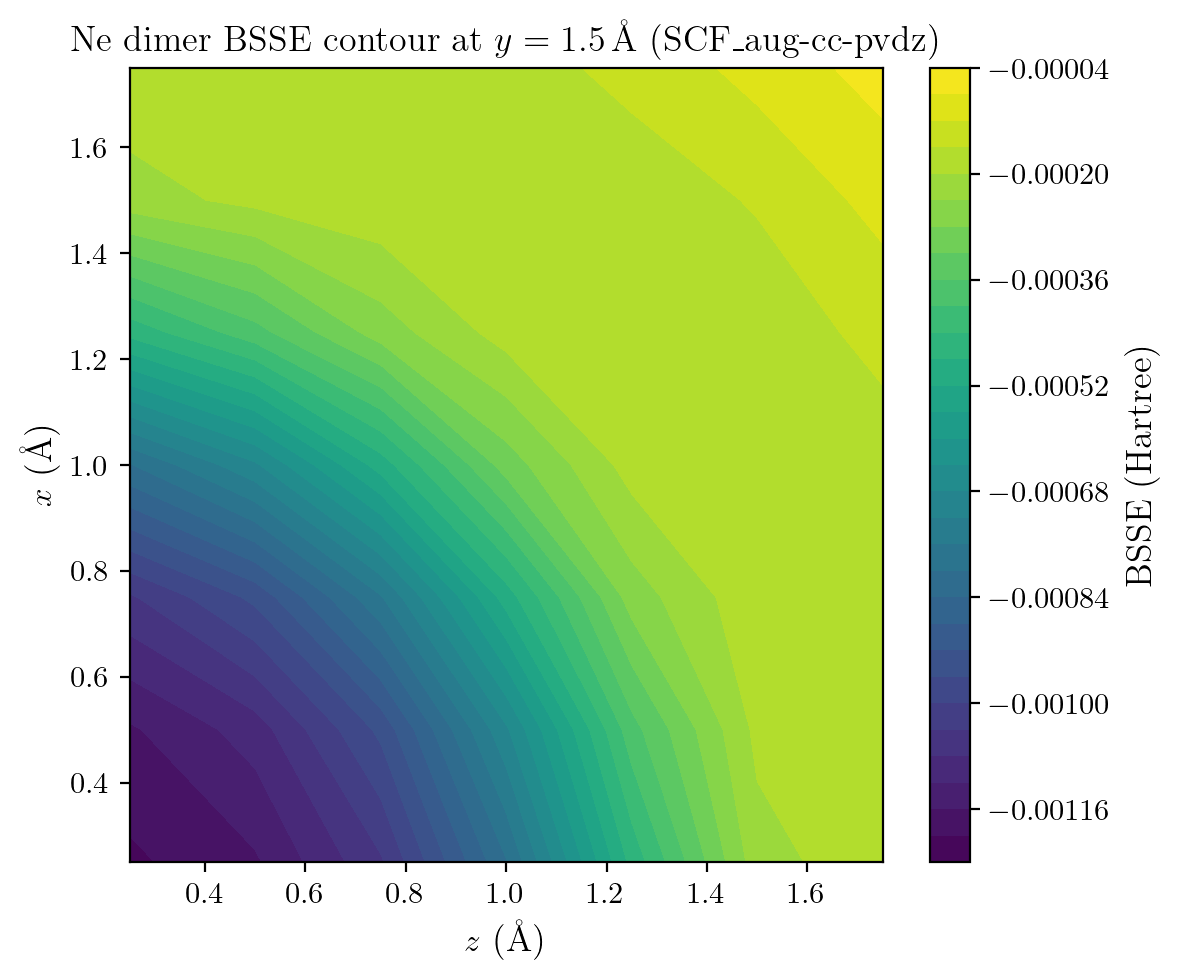
\includegraphics[width=\textwidth]{figures/dimer/Ne_dimer/Ne_trnl_contour_1.5_SCF.png}
        \caption{SCF, $y = \SI{1.5}{\angstrom}$}
    \end{subfigure}
    \hfill
    \begin{subfigure}[b]{0.32\textwidth}
        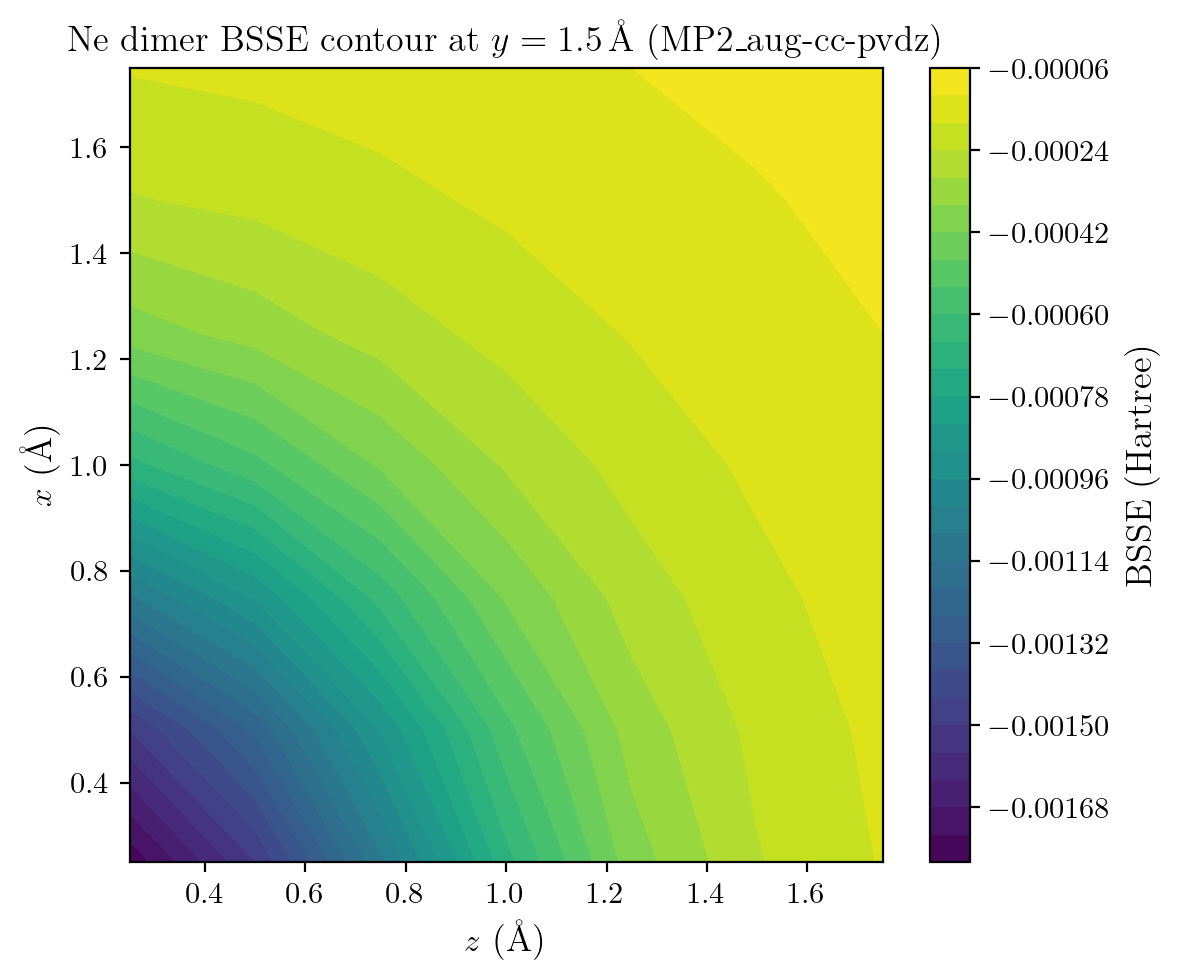
\includegraphics[width=\textwidth]{figures/dimer/Ne_dimer/Ne_trnl_contour_1.5_MP2.png}
        \caption{MP2 corr., $y = \SI{1.5}{\angstrom}$}
    \end{subfigure}
    \hfill
    \begin{subfigure}[b]{0.32\textwidth}
        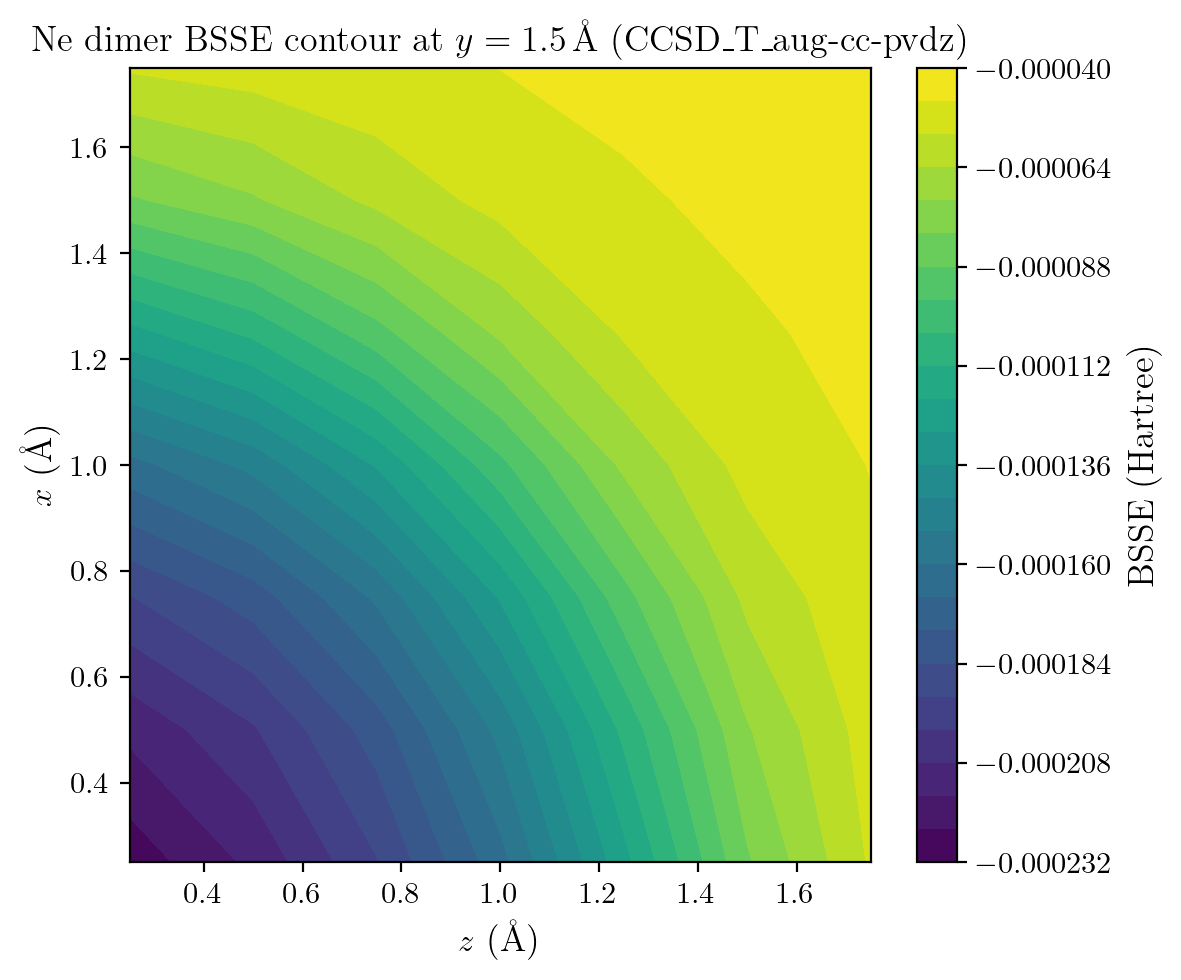
\includegraphics[width=\textwidth]{figures/dimer/Ne_dimer/Ne_trnl_contour_1.5_CCSD_T.png}
        \caption{CCSD(T) corr., $y = \SI{1.5}{\angstrom}$}
    \end{subfigure}

    \vspace{0.8em}

    \begin{subfigure}[b]{0.32\textwidth}
        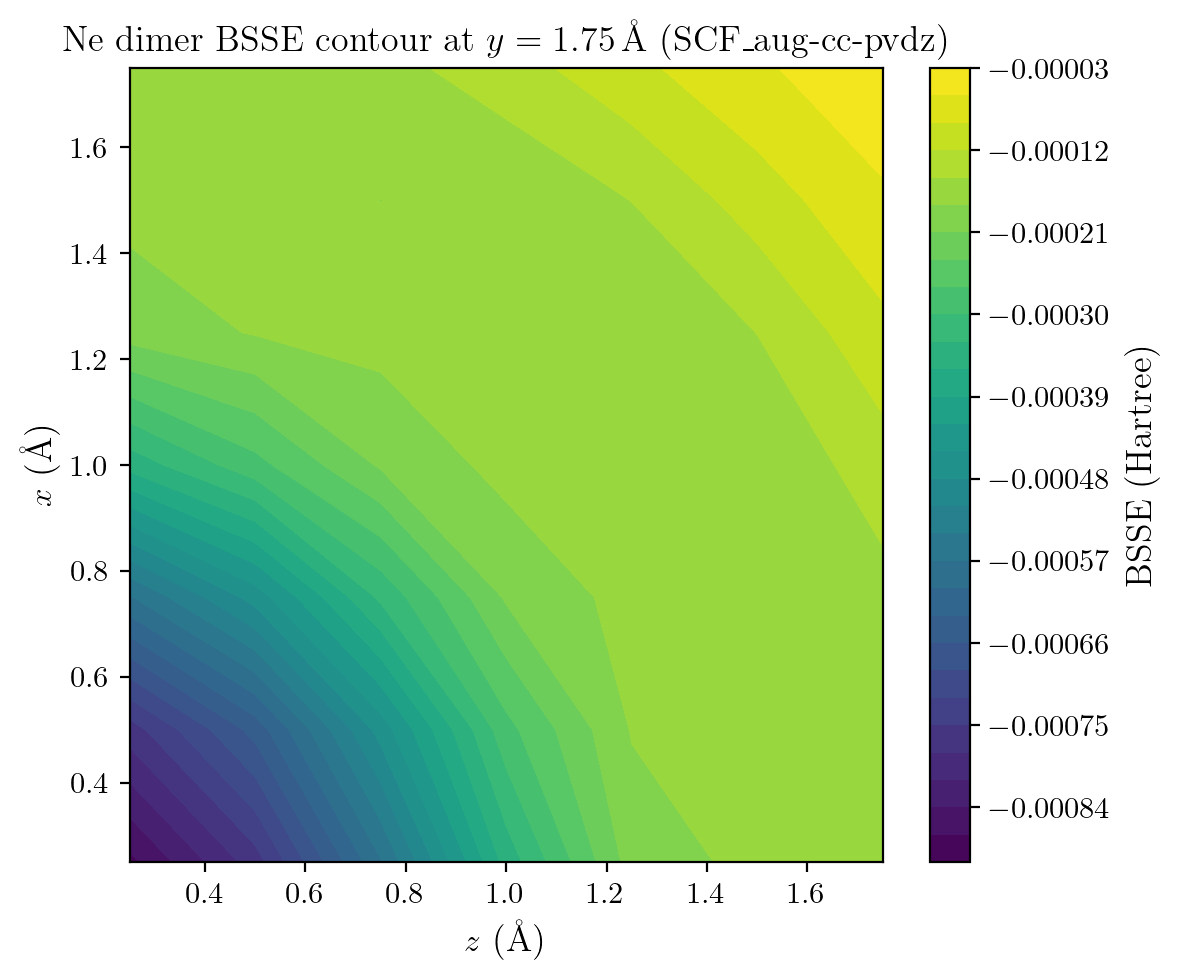
\includegraphics[width=\textwidth]{figures/dimer/Ne_dimer/Ne_trnl_contour_1.75_SCF.png}
        \caption{SCF, $y = \SI{1.75}{\angstrom}$}
    \end{subfigure}
    \hfill
    \begin{subfigure}[b]{0.32\textwidth}
        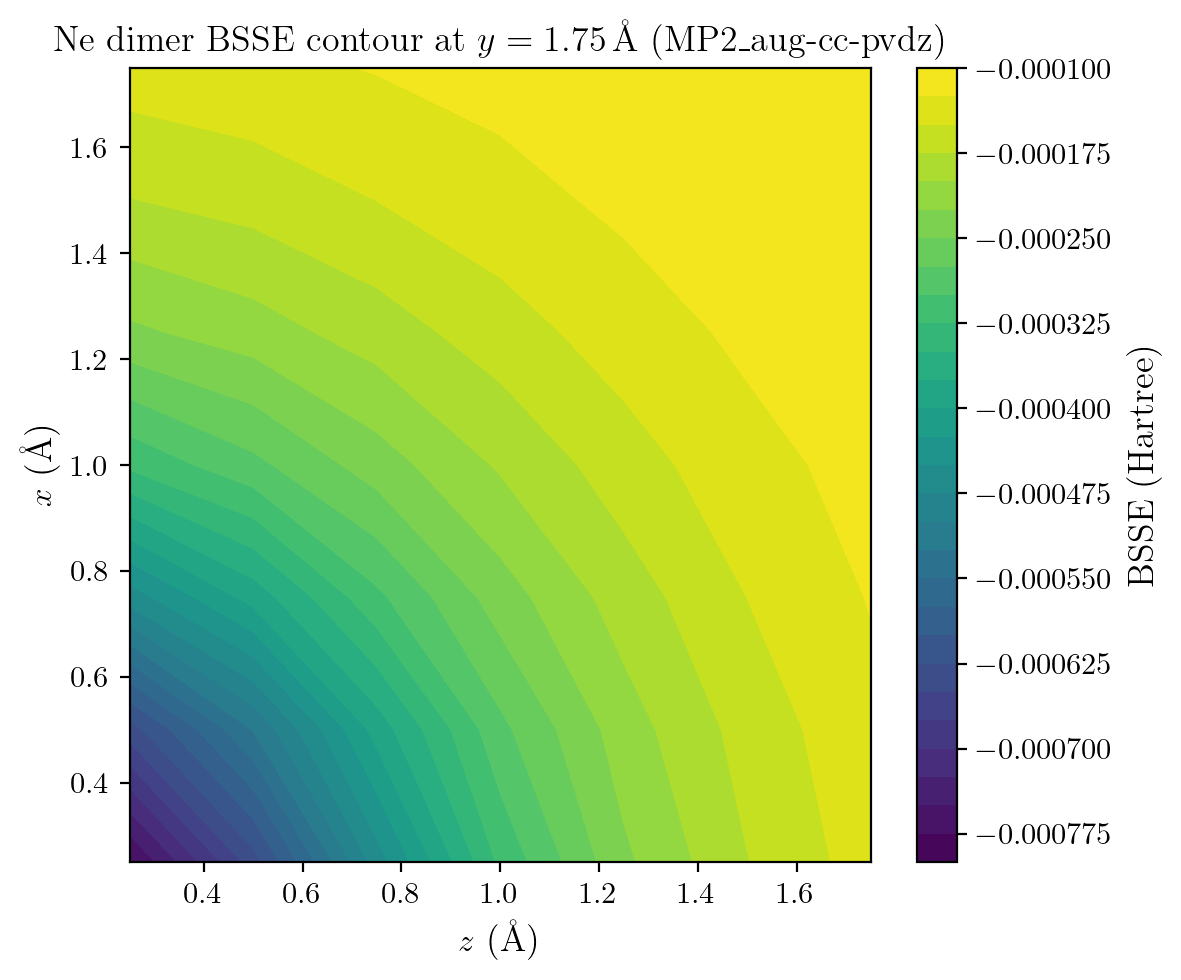
\includegraphics[width=\textwidth]{figures/dimer/Ne_dimer/Ne_trnl_contour_1.75_MP2.png}
        \caption{MP2 corr., $y = \SI{1.75}{\angstrom}$}
    \end{subfigure}
    \hfill
    \begin{subfigure}[b]{0.32\textwidth}
        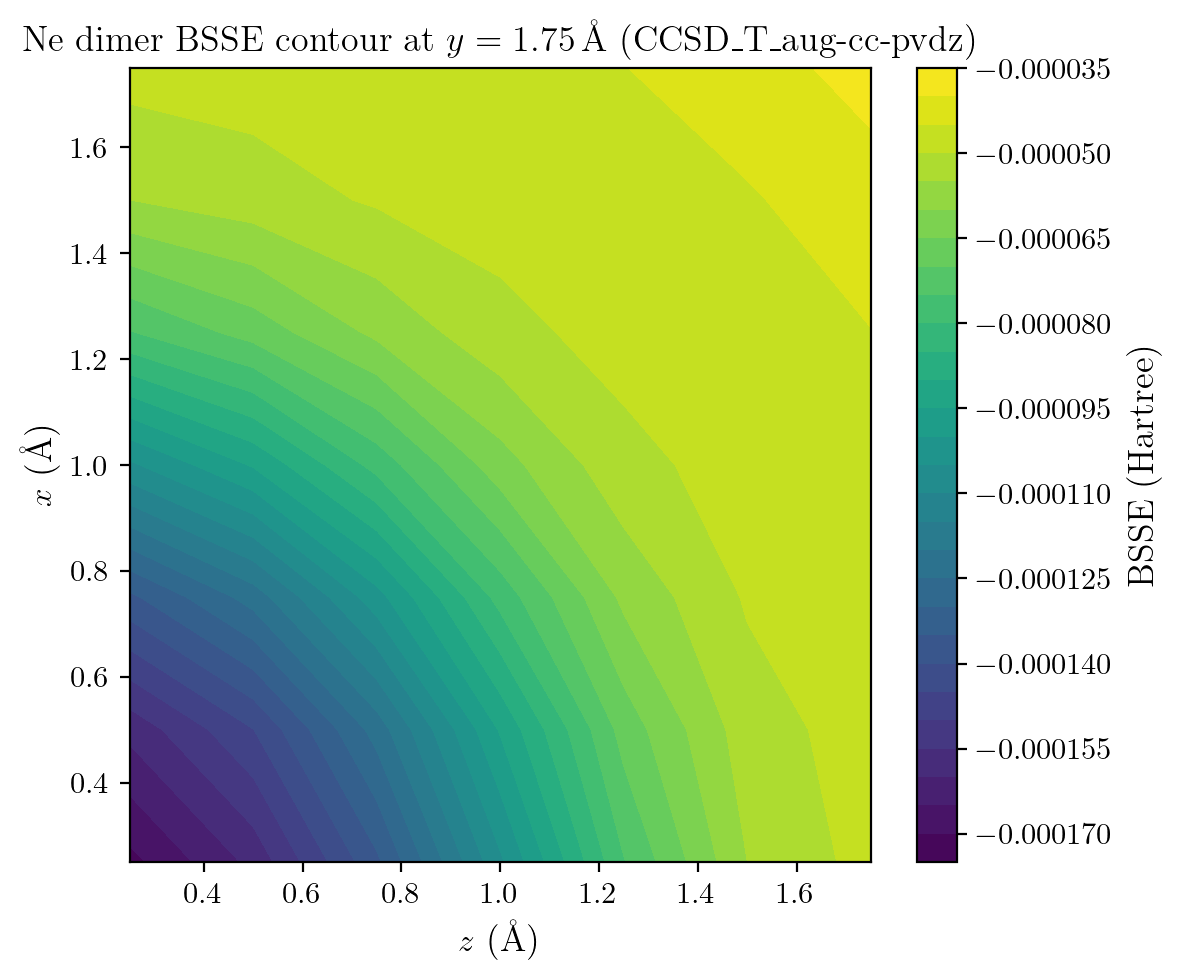
\includegraphics[width=\textwidth]{figures/dimer/Ne_dimer/Ne_trnl_contour_1.75_CCSD_T.png}
        \caption{CCSD(T) corr., $y = \SI{1.75}{\angstrom}$}
    \end{subfigure}

    \caption{BSSE contour plots for the Ne dimer translational scan at
    fixed $y = 1.5$ and \SI{1.75}{\angstrom}. Axes correspond to the
    in-plane Ne--Ne displacement components $(x, z)$ in \AA. Contour
    levels represent the BSSE in Hartree. The MP2 and CCSD(T) labels
    refer to the correlation energy components relative to SCF and MP2,
    respectively. The perfectly circular contour arcs confirm that BSSE
    depends only on the Ne--Ne separation $R$, with no orientational
    dependence, consistent with the spherical symmetry of the Ne atom.}
    \label{fig:ne_trnl_contours}
\end{figure}

The contour plots show perfectly circular arcs centered on the origin
at both $y$ values and across all three levels of theory. This confirms
that BSSE in the Ne dimer is a function only of the Ne--Ne distance
$R = |\mathbf{r}|$, with no dependence on the direction of the
displacement vector. The result is physically expected from the
spherical symmetry of Ne and serves as an important validation of the
computational setup.

Comparing the three methods, the MP2 correlation component shows the
largest BSSE magnitude, while the CCSD(T) increment beyond MP2 is
small. This ordering --- SCF $<$ CCSD(T) corr.\ $\ll$ MP2 corr.\ ---
is consistent across both $y$ slices and is characteristic of
correlated wavefunction methods applied to diffuse basis sets.

% ----------------------------------------------------------------------
\subsection{Key Findings}
% ----------------------------------------------------------------------

\begin{finding_box}
\textbf{Ne dimer BSSE is purely radial.}
The translational contour plots show perfectly circular arcs at both
sampled $y$ values and across all three levels of theory. BSSE in the
Ne dimer depends exclusively on the Ne--Ne separation $R$ with no
orientational dependence, as expected from the spherical symmetry of
the Ne atom. This result establishes a clean radial baseline against
which the orientational behavior of the polyatomic dimers (\ce{H2O}
and HF) can be compared.
\end{finding_box}

\begin{finding_box}
\textbf{MP2 correlation dominates the Ne dimer BSSE.}
Decomposing the total BSSE into SCF, MP2 correlation, and CCSD(T)
correlation components reveals that the MP2 contribution is the
largest at all sampled geometries. The CCSD(T) increment beyond MP2
is small. This energy decomposition hierarchy is consistent across
both $y$ slices and will be seen again in the \ce{H2O} and HF dimers.
\end{finding_box}

\clearpage

% ======================================================================
\section{\ce{H2O} Dimer}
% ======================================================================

% ----------------------------------------------------------------------
\subsection{Overview}
% ----------------------------------------------------------------------

The \ce{H2O} dimer serves as the central polyatomic case for this
study. Two complementary sampling strategies were employed to
characterize how BSSE depends on the relative geometry of the two
monomers: a \textit{translational scan}, in which monomer B is
displaced along a three-dimensional grid while monomer A remains
fixed, and a \textit{rotational--radial scan}, in which the Euler
angles $(\alpha, \beta, \gamma)$ of monomer B are sampled randomly
while the O--O separation $R$ is varied independently. All
calculations were performed at the SCF, MP2, and CCSD(T) levels using
the aug-cc-pVDZ basis set~\cite{dunning1989,kendall1992} with the
NWChem quantum chemistry package~\cite{nwchem2020}.

The BSSE for each dimer configuration is computed as in
Eq.~\eqref{eq:ne_dimer_bsse}, with $A$ and $B$ now denoting the two
\ce{H2O} monomers. Energies are reported in Hartree and distances
in \AA.

% ----------------------------------------------------------------------
\subsection{Experimental Design}
% ----------------------------------------------------------------------

\subsubsection{Monomer Geometry}

Both monomers use a rigid \ce{H2O} geometry. Monomer A is placed at
the origin with its oxygen atom and two hydrogen atoms fixed in the
$xy$ plane for all calculations. All coordinates are given in \AA,
consistent with the NWChem default convention.

\subsubsection{Translational Scan}

In the translational scan, the O--O displacement vector
$\mathbf{r} = \mathbf{r}_2 - \mathbf{r}_1$ (from the oxygen of
monomer A to the oxygen of monomer B) is varied in increments of
\SI{0.25}{\angstrom}. The scan is organized into three families of
two-dimensional slices:
\begin{itemize}
    \item Fixed $x$: contour over $(y, z)$
    \item Fixed $y$: contour over $(x, z)$
    \item Fixed $z$: contour over $(x, y)$
\end{itemize}
Only the fixed-$y$ slices at $y = 2.0$, $2.25$, $2.50$, and
\SI{2.75}{\angstrom} form complete $7 \times 7$ grids (49 points each)
and are used for contour analysis. The fixed-$x$ and fixed-$z$
families have incomplete grids and are excluded from the contour plots.

\subsubsection{Rotational--Radial Scan}

In the rotational--radial scan, the Euler angles $(\alpha, \beta,
\gamma)$ of monomer B are sampled randomly, producing 64 unique
orientations. For each orientation, the O--O separation $R$ is varied
independently. A total of 288 data points per method were collected.
Of the 64 orientations, 32 have at least 5 distinct $R$ values and
are used for plotting BSSE vs $R$ curves.

% ----------------------------------------------------------------------
\subsection{Translational Scan Results}
% ----------------------------------------------------------------------

Figure~\ref{fig:h2o_trnl_contours} shows the BSSE contour plots for
the fixed-$y$ slices at $y = 2.50$ and \SI{2.75}{\angstrom} for all
three levels of theory. Each panel shows BSSE as a function of the
in-plane coordinates $(x, z)$.

\begin{figure}[!ht]
    \centering
    \begin{subfigure}[b]{0.32\textwidth}
        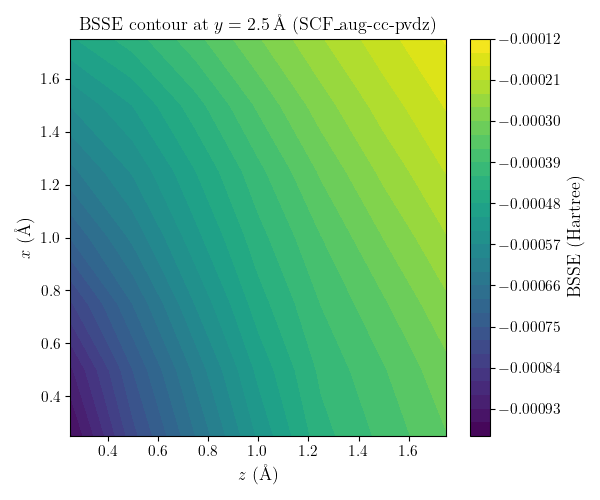
\includegraphics[width=\textwidth]{figures/dimer/H2O_dimer/H2O_trnl_contour_2.50_SCF.png}
        \caption{SCF, $y = \SI{2.50}{\angstrom}$}
    \end{subfigure}
    \hfill
    \begin{subfigure}[b]{0.32\textwidth}
        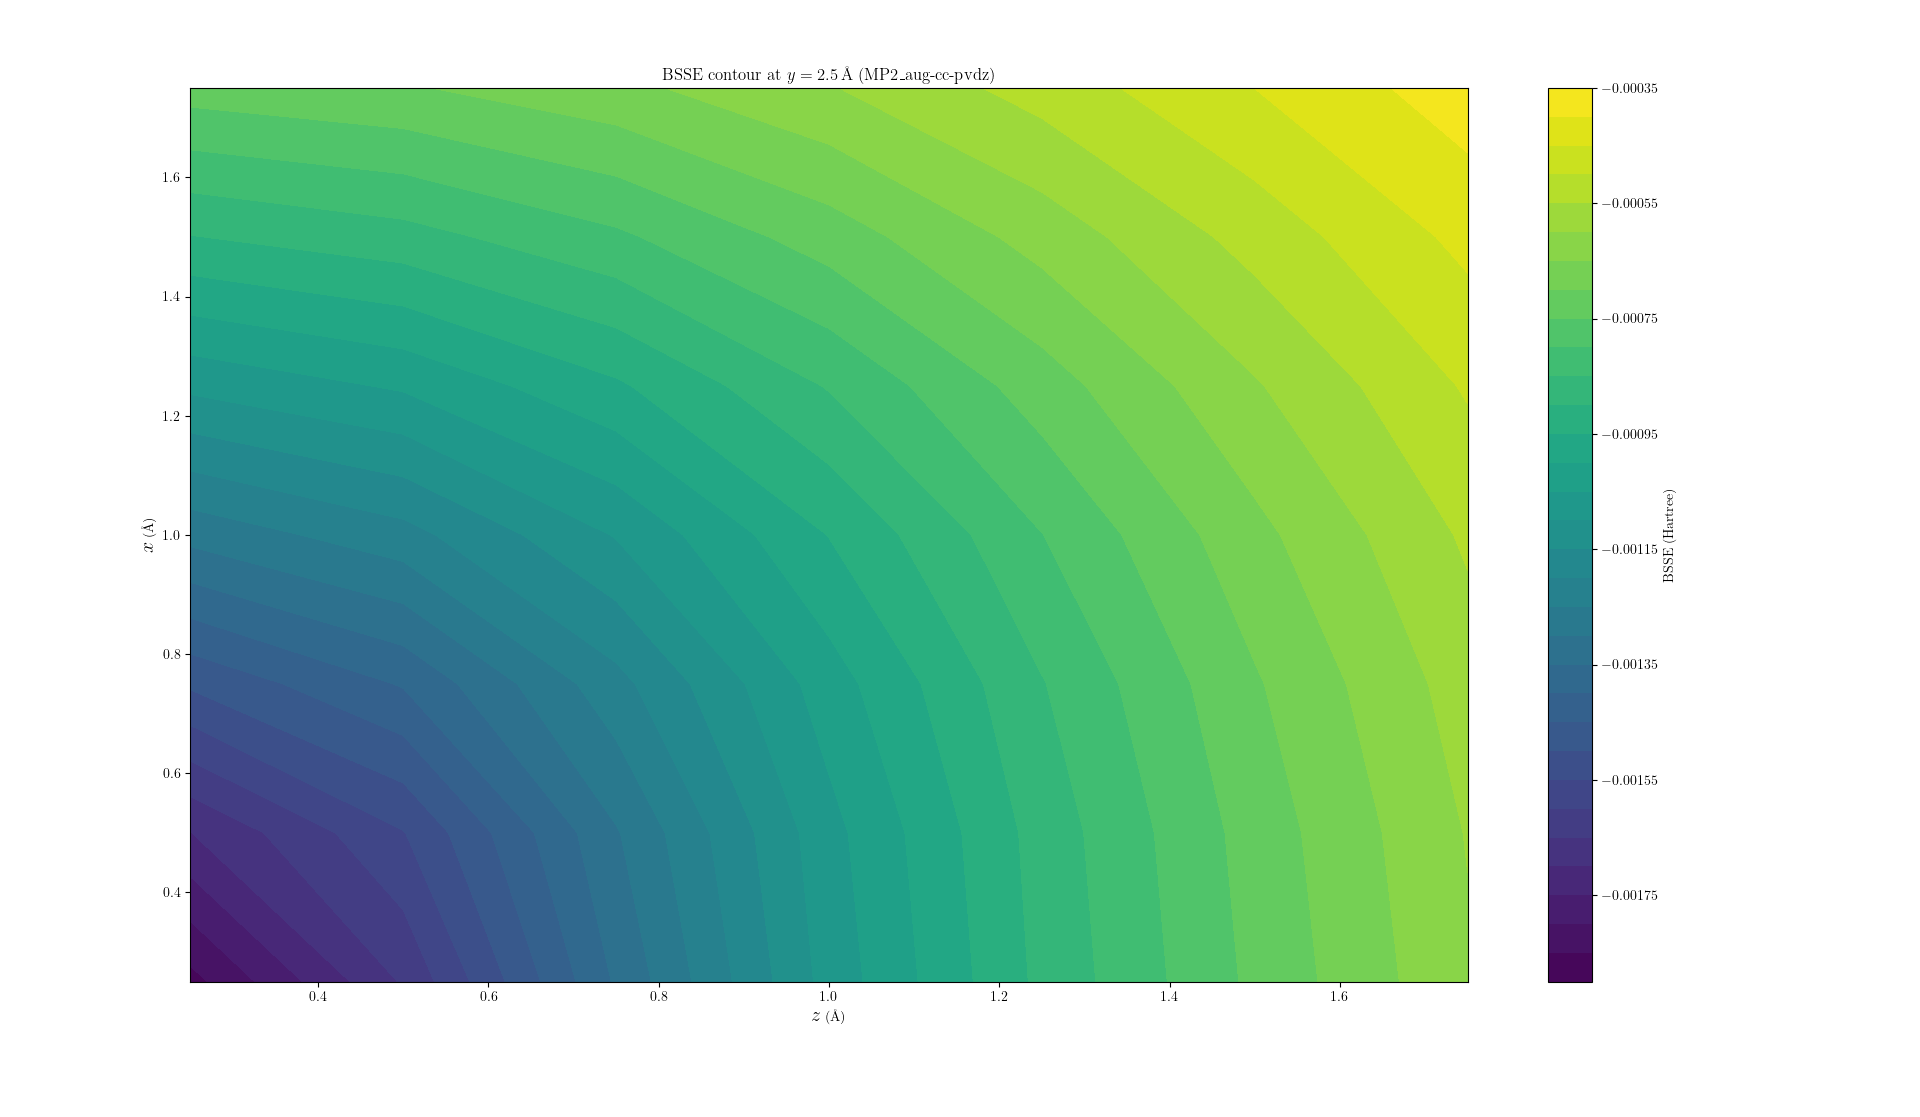
\includegraphics[width=\textwidth]{figures/dimer/H2O_dimer/H2O_trnl_contour_2.50_MP2.png}
        \caption{MP2 corr., $y = \SI{2.50}{\angstrom}$}
    \end{subfigure}
    \hfill
    \begin{subfigure}[b]{0.32\textwidth}
        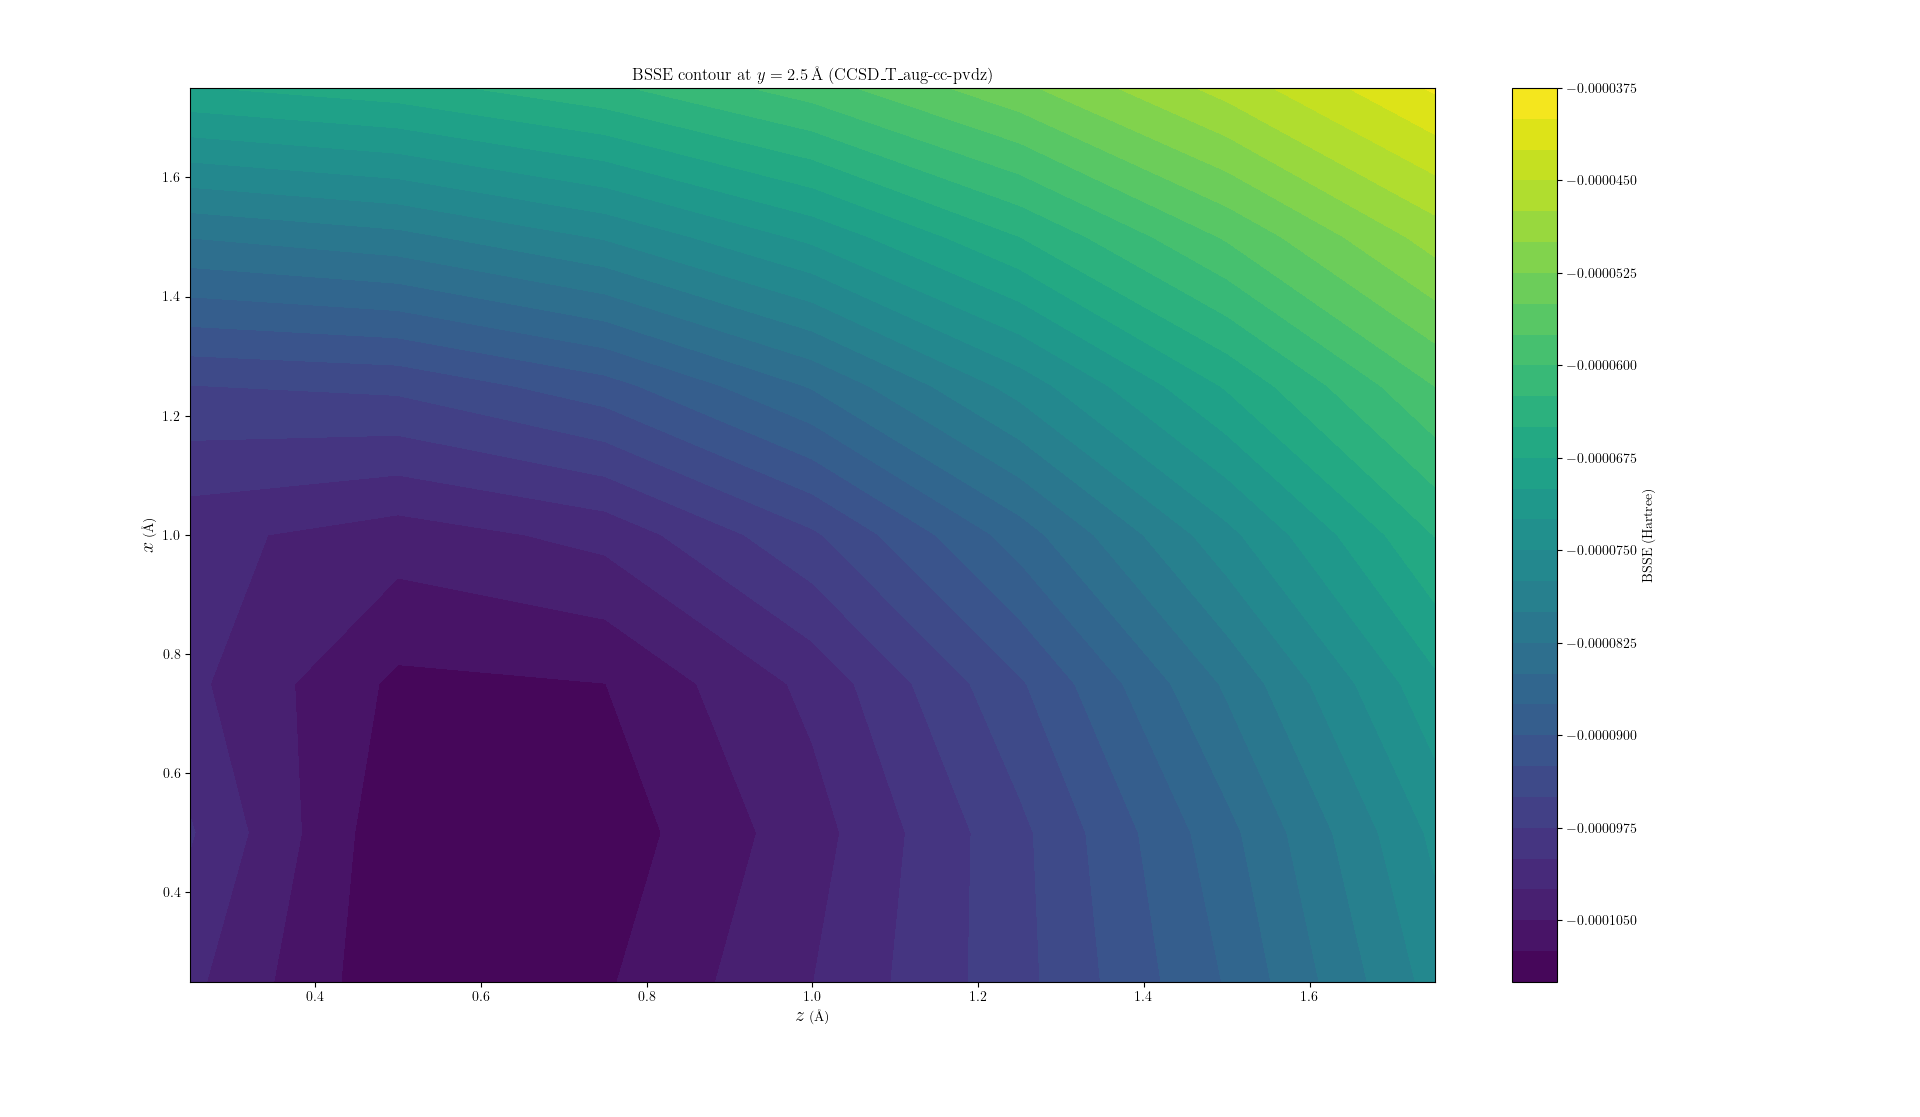
\includegraphics[width=\textwidth]{figures/dimer/H2O_dimer/H2O_trnl_contour_2.50_CCSD_T.png}
        \caption{CCSD(T) corr., $y = \SI{2.50}{\angstrom}$}
    \end{subfigure}

    \vspace{0.8em}

    \begin{subfigure}[b]{0.32\textwidth}
        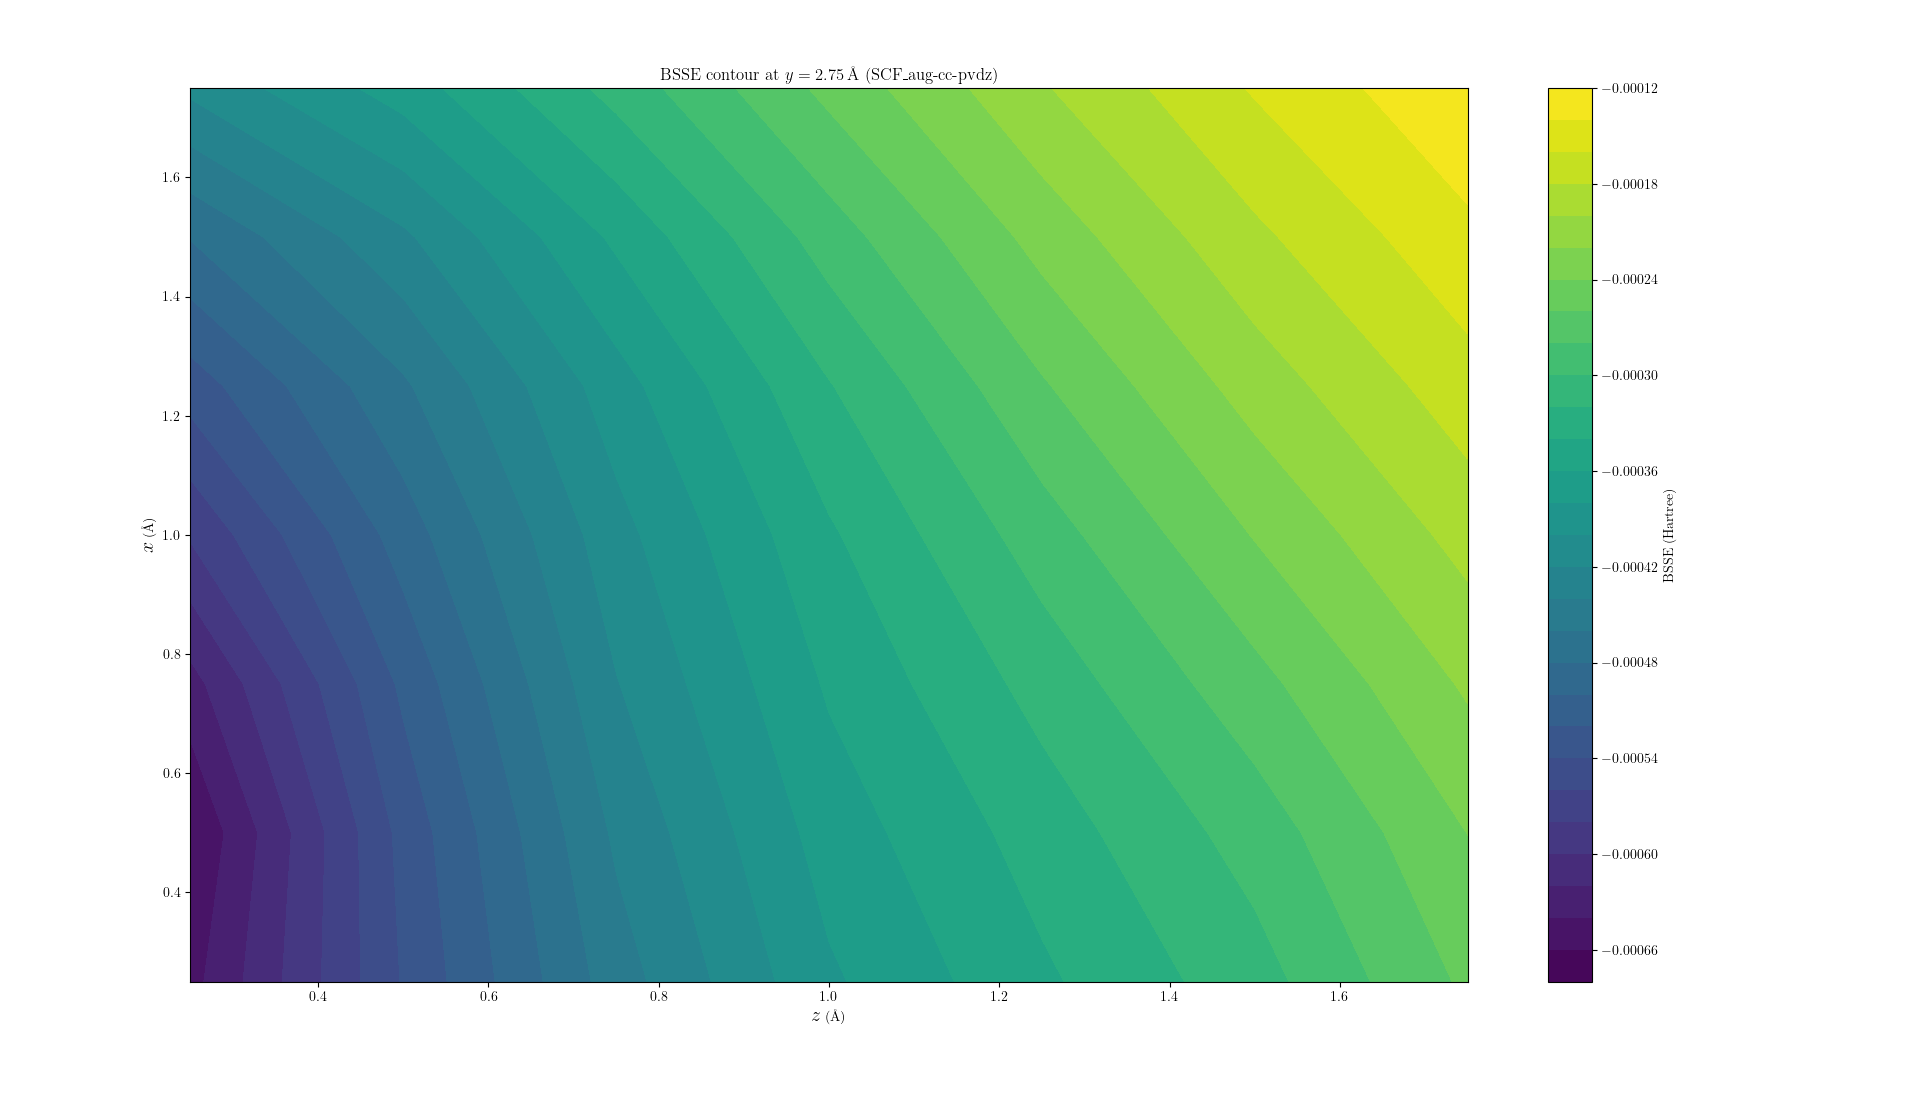
\includegraphics[width=\textwidth]{figures/dimer/H2O_dimer/H2O_trnl_contour_2.75_SCF.png}
        \caption{SCF, $y = \SI{2.75}{\angstrom}$}
    \end{subfigure}
    \hfill
    \begin{subfigure}[b]{0.32\textwidth}
        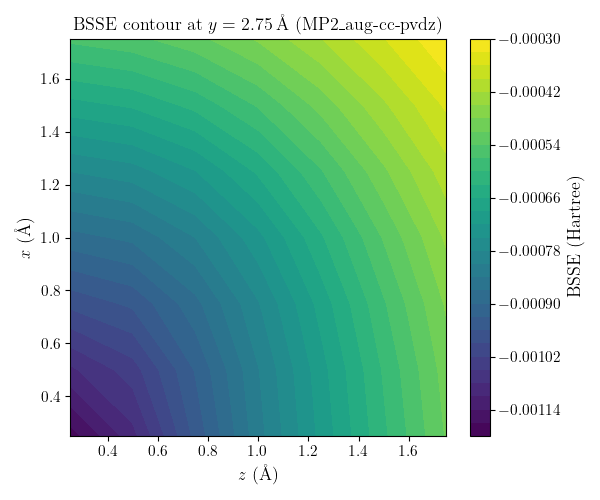
\includegraphics[width=\textwidth]{figures/dimer/H2O_dimer/H2O_trnl_contour_2.75_MP2.png}
        \caption{MP2 corr., $y = \SI{2.75}{\angstrom}$}
    \end{subfigure}
    \hfill
    \begin{subfigure}[b]{0.32\textwidth}
        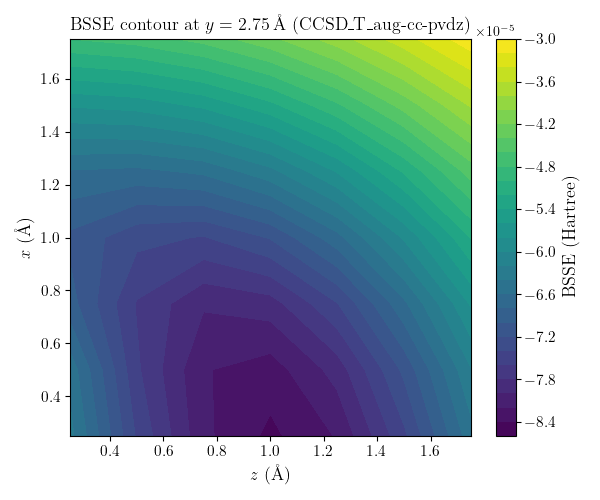
\includegraphics[width=\textwidth]{figures/dimer/H2O_dimer/H2O_trnl_contour_2.75_CCSD_T.png}
        \caption{CCSD(T) corr., $y = \SI{2.75}{\angstrom}$}
    \end{subfigure}

    \caption{BSSE contour plots for the \ce{H2O} dimer translational
    scan at fixed $y = 2.50$ and \SI{2.75}{\angstrom}. Axes correspond
    to the in-plane O--O displacement components $(x, z)$ in \AA.
    Contour levels represent the BSSE in Hartree. The MP2 and CCSD(T)
    labels refer to the correlation energy components relative to SCF
    and MP2, respectively. The nearly circular contour arcs indicate
    that BSSE depends primarily on the O--O separation $R$ with weak
    orientation dependence.}
    \label{fig:h2o_trnl_contours}
\end{figure}

The contour plots reveal nearly circular arcs centered on the origin,
indicating that BSSE is predominantly a function of the O--O distance
$R = |\mathbf{r}|$ with only weak dependence on the direction of the
displacement vector. This observation holds across all three levels of
theory and all four fixed-$y$ slices. In contrast to the Ne dimer,
the contours are not perfectly circular --- a small but visible
deviation from circular symmetry reflects the non-spherical geometry
of the \ce{H2O} monomer.

% ----------------------------------------------------------------------
\subsection{Rotational--Radial Scan Results}
% ----------------------------------------------------------------------

Figure~\ref{fig:h2o_rot_bsse_vs_R} shows $|\text{BSSE}|$ as a
function of $R$ for 9 representative orientations, with SCF, MP2
correlation, and CCSD(T) correlation components overlaid on each
panel.

Several observations are consistent across all 9 orientations:

\begin{enumerate}
    \item \textbf{Monotonic decay with $R$.} All three components
    decrease monotonically as the O--O separation increases,
    approaching zero at large $R$.

    \item \textbf{Dominance of the MP2 correlation component.} The
    MP2 correlation contribution to BSSE is the largest of the three
    components across all orientations and distances sampled.
    % At the
    % SCF level, only the occupied molecular orbitals contribute to the
    % electron density, and the basis set incompleteness error arises
    % from the inability of the monomer's own basis to describe these
    % occupied orbitals in the field of the partner. At the MP2 level,
    % the correlation energy is computed through excitations into virtual
    % orbitals, which are typically more diffuse and more sensitive to
    % basis set incompleteness than the occupied orbitals. As a result,
    % the correlated wavefunction benefits more from borrowing the
    % partner's basis functions --- the ghost atoms effectively provide
    % additional virtual space that the monomer's own basis lacks. This
    % amplification of BSSE by electron correlation is a well-known
    % phenomenon and is one of the primary motivations for using
    % augmented basis sets such as aug-cc-pVDZ in BSSE studies.

    \item \textbf{Small CCSD(T) increment.} The CCSD(T) correlation
    component is consistently small relative to both SCF and MP2
    contributions.
    % suggesting that higher-order correlation effects
    % beyond MP2 contribute minimally to the BSSE.

    \item \textbf{Weak orientation dependence.} The shape and
    magnitude of the BSSE curves are consistent across different
    $(\alpha, \beta, \gamma)$ values, in agreement with the nearly
    circular contour arcs observed in the translational scan.
\end{enumerate}

\vspace{0.25cm}
\begin{figure}[!ht]
    \centering
    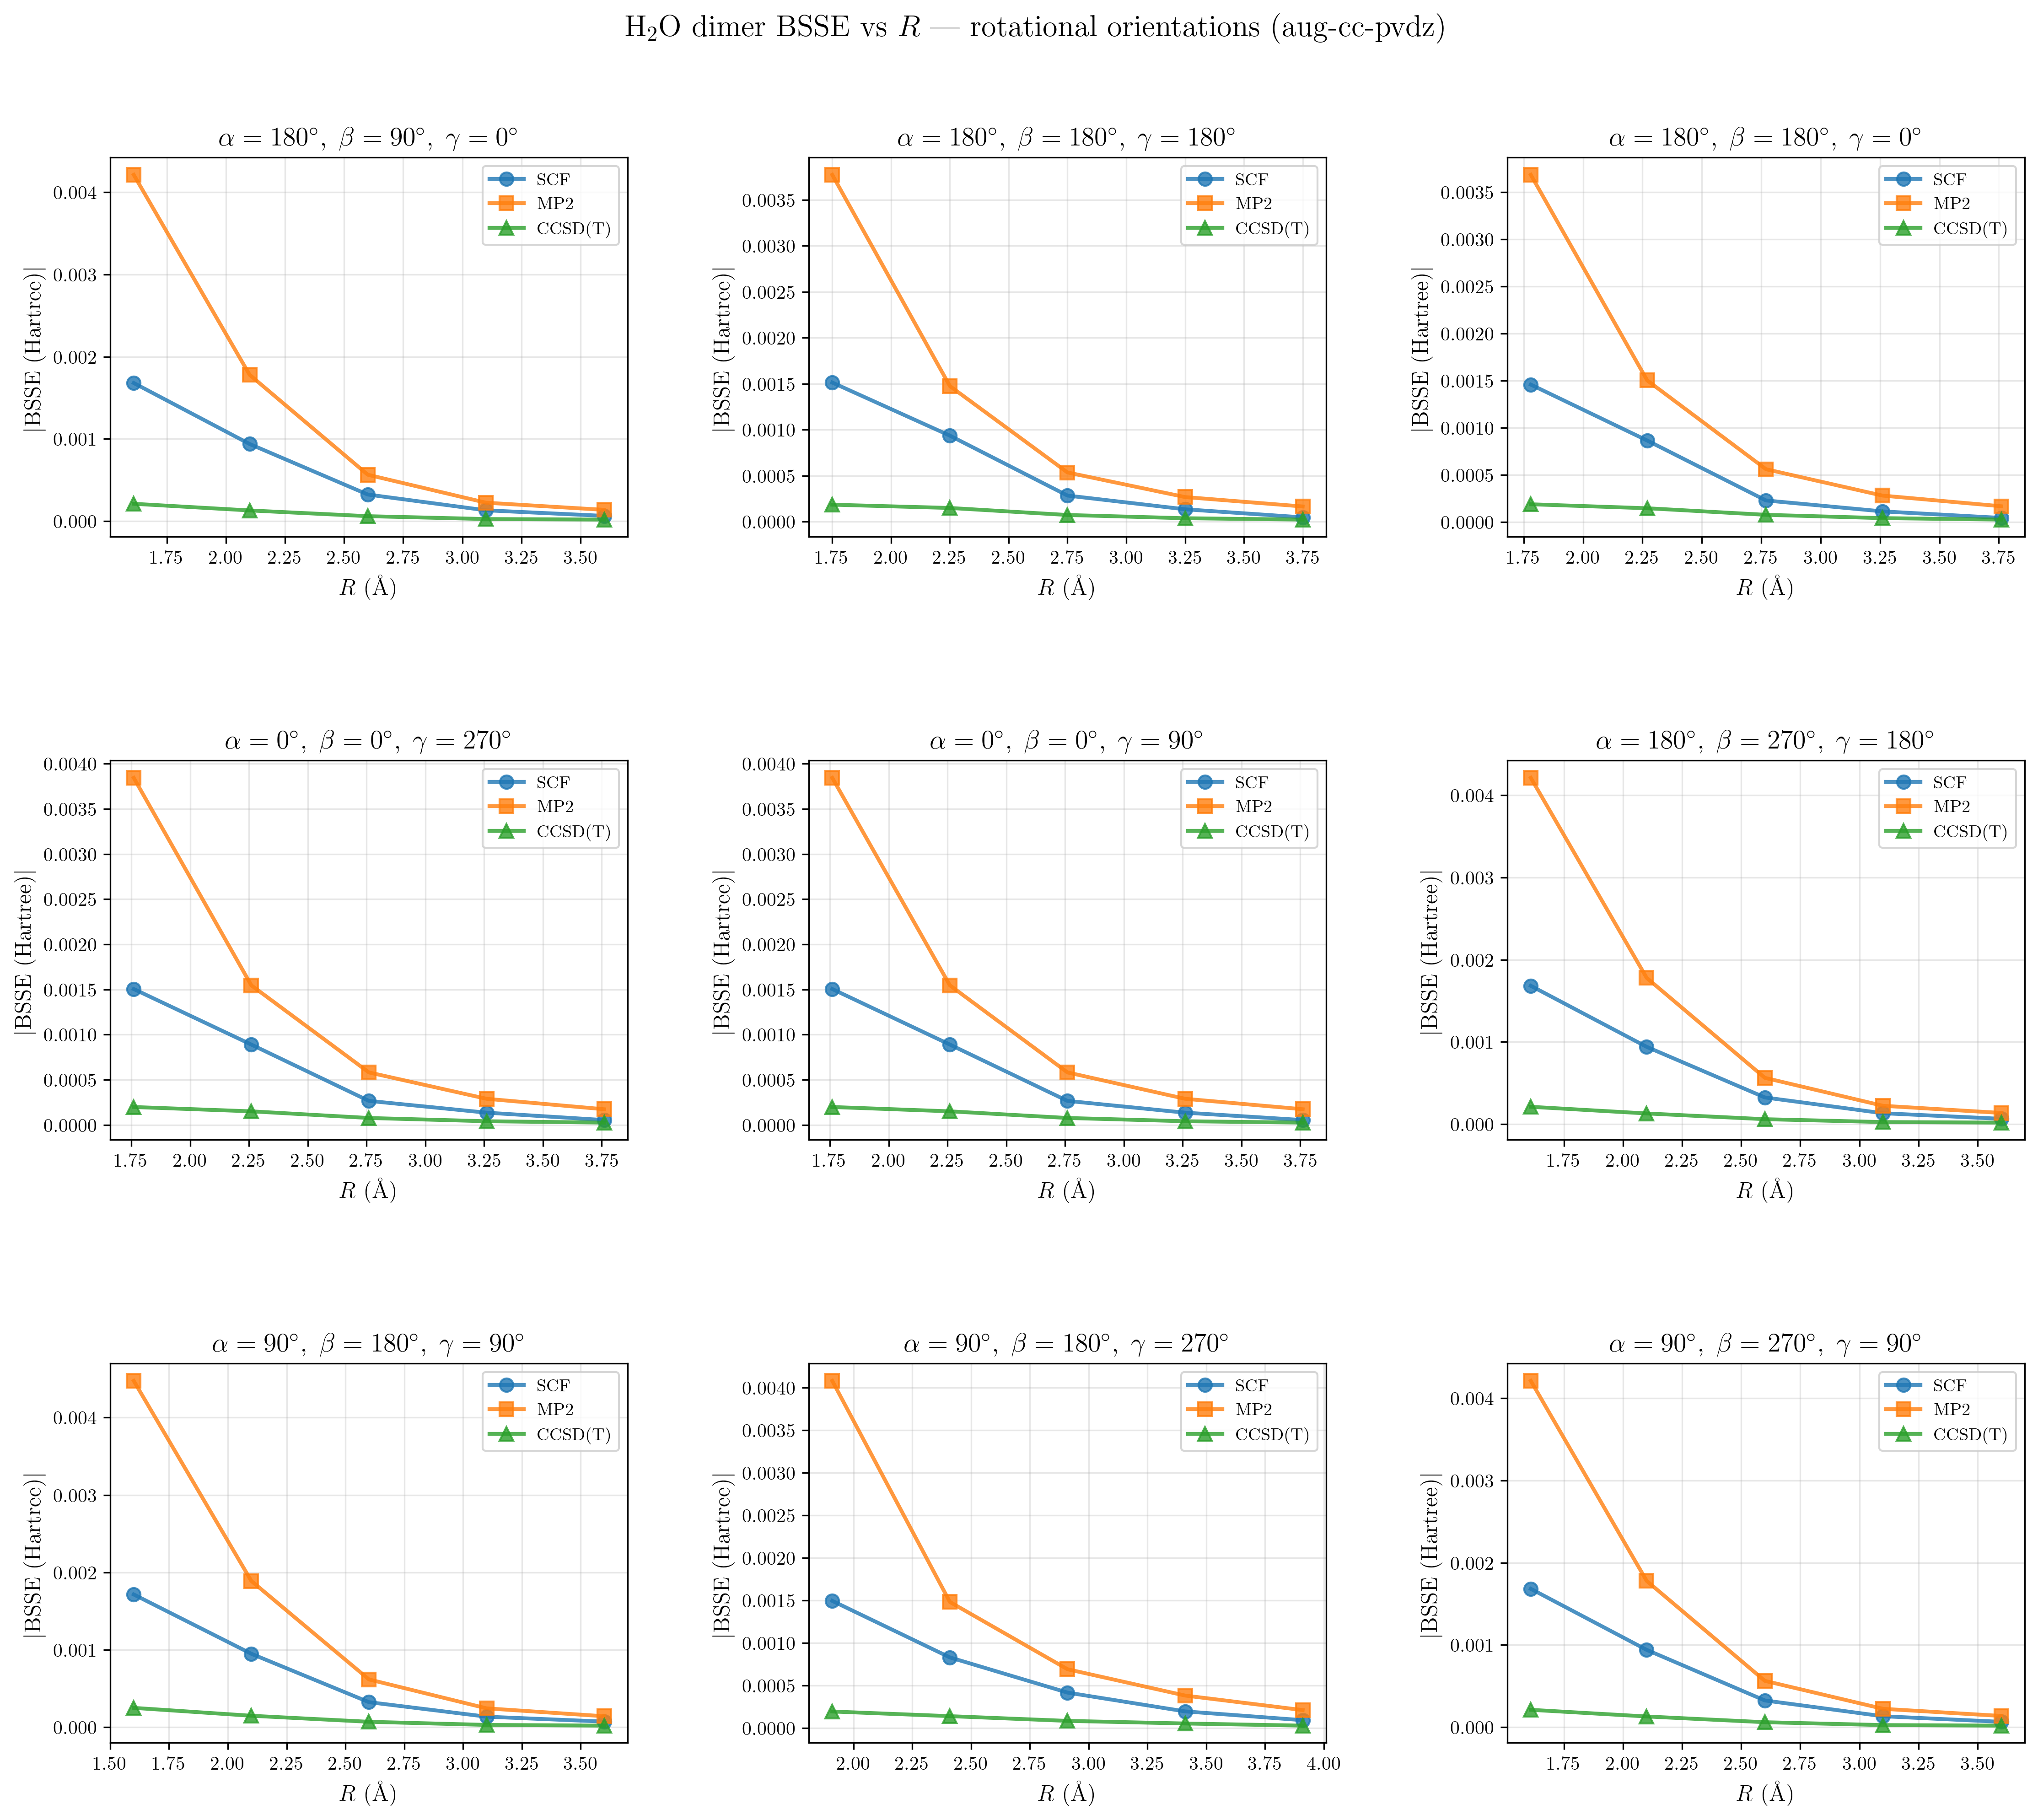
\includegraphics[width=1.0\textwidth]{figures/dimer/H2O_dimer/H2O_rot_vs_R_SCFMP2CCSD_T.png}
    \caption{$|\text{BSSE}|$ vs O--O separation $R$ for 9
    representative rotational orientations of the \ce{H2O} dimer at
    the aug-cc-pVDZ level. Each panel corresponds to a distinct set of
    Euler angles $(\alpha, \beta, \gamma)$ as labeled. Blue circles:
    SCF contribution; orange squares: MP2 correlation component
    ($E_\text{MP2} - E_\text{SCF}$); green triangles: CCSD(T)
    correlation component ($E_{\text{CCSD(T)}} - E_\text{MP2}$).
    All three components decay monotonically with $R$ and show
    consistent behavior across orientations, confirming weak
    orientation dependence of dimer BSSE.}
    \label{fig:h2o_rot_bsse_vs_R}
\end{figure}

\clearpage

% ----------------------------------------------------------------------
\subsection{Key Findings}
% ----------------------------------------------------------------------

\begin{finding_box}
\textbf{\ce{H2O} dimer BSSE is primarily a function of O--O distance.}
Both the translational contour plots and the rotational--radial scan
confirm that BSSE in the \ce{H2O} dimer depends weakly on the relative
orientation of the monomers and is governed primarily by the O--O
separation $R$. The nearly circular contour arcs represent a modest
deviation from the perfect circular symmetry seen in the Ne dimer,
consistent with the non-spherical geometry of the \ce{H2O} monomer.
% This result motivates the hypothesis that a simple
% distance-based threshold could be used to identify configurations
% where BSSE corrections are negligible.
\end{finding_box}

\begin{finding_box}
\textbf{MP2 correlation dominates the \ce{H2O} dimer BSSE.}
Decomposing the total BSSE into SCF, MP2 correlation, and CCSD(T)
correlation components reveals that the MP2 contribution is the
largest at all sampled distances and orientations. The CCSD(T)
correction beyond MP2 is small.
% This energy decomposition hierarchy
% provides essential context for the trimer analysis presented in
% Chapters~\ref{ch:trimer_bsse} and~\ref{ch:trimer_interaction}.
\end{finding_box}

\clearpage

% ======================================================================
\section{HF Dimer}
% ======================================================================

% ----------------------------------------------------------------------
\subsection{Overview}
% ----------------------------------------------------------------------

The HF dimer completes the set of three dimer systems studied in this
work. As a polar, heteronuclear diatomic, HF introduces a qualitative
distinction from both Ne and \ce{H2O}: the two ends of the molecule
are chemically inequivalent, so the direction of the displacement
vector relative to the HF bond axis can in principle affect the BSSE.
Two complementary sampling strategies were employed, mirroring the
\ce{H2O} analysis: a \textit{translational scan}, in which monomer B
is displaced along a three-dimensional grid while monomer A remains
fixed, and a \textit{rotational--radial scan}, in which the Euler
angles $(\alpha, \beta, \gamma)$ of monomer B are varied
systematically while the F--F separation $R$ is held fixed. All
calculations were performed at the SCF, MP2, and CCSD(T) levels using
the aug-cc-pVDZ basis set~\cite{dunning1989,kendall1992} with the
NWChem quantum chemistry package~\cite{nwchem2020}.

The BSSE for each dimer configuration is computed as in
Eq.~\eqref{eq:ne_dimer_bsse}, with $A$ and $B$ now denoting the two
HF monomers. Energies are reported in Hartree and distances in \AA.

% ----------------------------------------------------------------------
\subsection{Experimental Design}
% ----------------------------------------------------------------------

\subsubsection{Monomer Geometry}

Monomer A is placed at the origin with the HF bond axis fixed in the
$xy$ plane for all calculations. The HF bond length is approximately
\SI{0.924}{\angstrom}. All coordinates are given in \AA, consistent
with the NWChem default convention.

\subsubsection{Translational Scan}

The translational scan follows the same protocol as the \ce{H2O}
dimer. The F--F displacement vector $\mathbf{r} = \mathbf{r}_2 -
\mathbf{r}_1$ is varied in increments of \SI{0.25}{\angstrom}. Only
the fixed-$y$ slices at $y = 1.5$ and $y = \SI{1.75}{\angstrom}$
form complete $7 \times 7$ grids (49 points each) and are used for
contour analysis. The axes of each contour plot correspond to the
in-plane F--F displacement components $(x, z)$ in \AA.

\subsubsection{Rotational--Radial Scan}

In the rotational--radial scan, the Euler angles of monomer B are
varied systematically rather than randomly. A total of 152
orientations were generated, all with $\alpha = 90.0°$. Of these, 28
have at least 5 distinct $R$ values and are used for plotting BSSE
vs $R$ curves. This systematic sampling contrasts with the random
Euler angle sampling used for \ce{H2O} and provides denser coverage
of a specific rotational subspace.

% ----------------------------------------------------------------------
\subsection{Translational Scan Results}
% ----------------------------------------------------------------------

Figure~\ref{fig:hf_trnl_contours} shows the BSSE contour plots for
the fixed-$y$ slices at $y = 1.5$ and \SI{1.75}{\angstrom} for all
three levels of theory.

\begin{figure}[!ht]
    \centering
    \begin{subfigure}[b]{0.32\textwidth}
        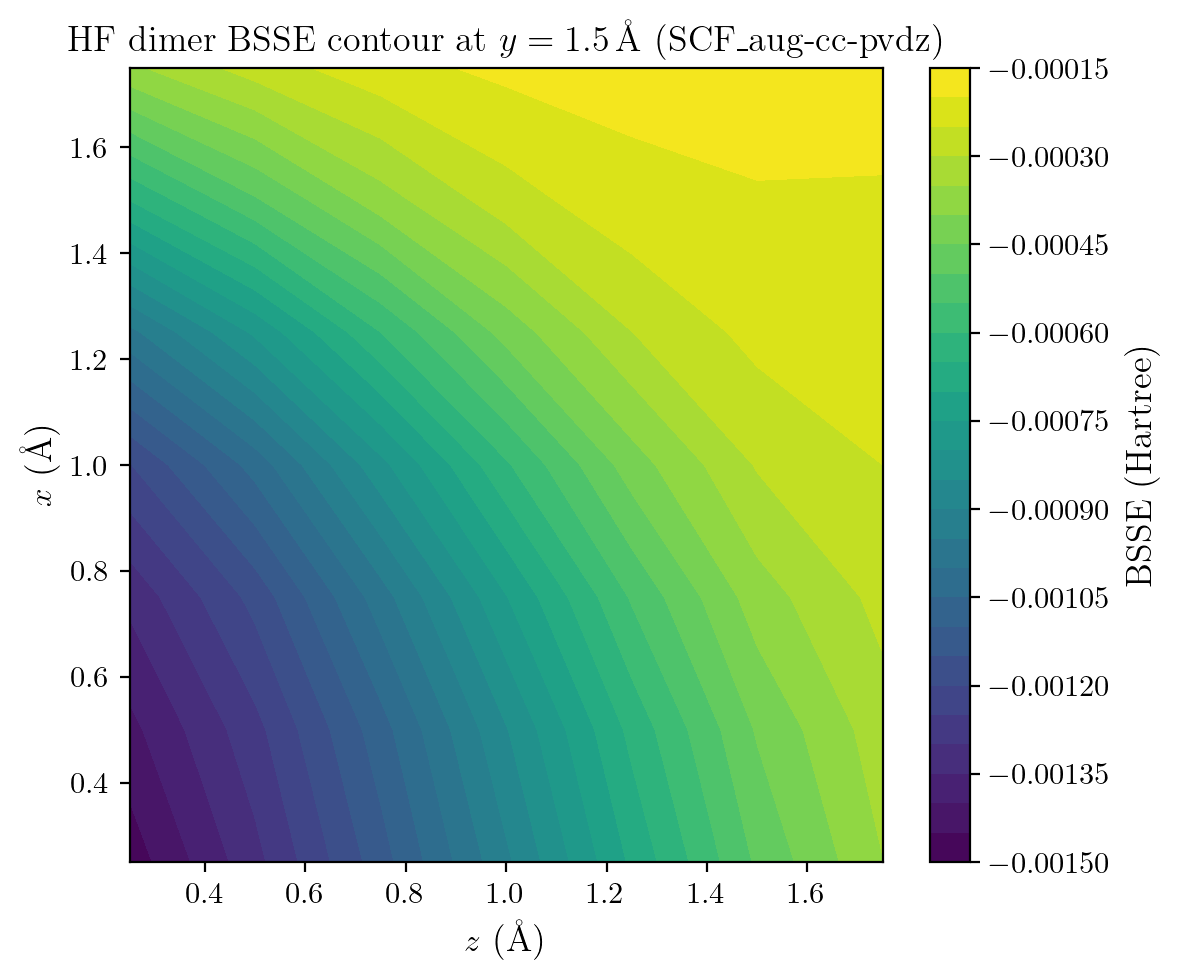
\includegraphics[width=\textwidth]{figures/dimer/HF_dimer/HF_trnl_contour_1.5_SCF.png}
        \caption{SCF, $y = \SI{1.5}{\angstrom}$}
    \end{subfigure}
    \hfill
    \begin{subfigure}[b]{0.32\textwidth}
        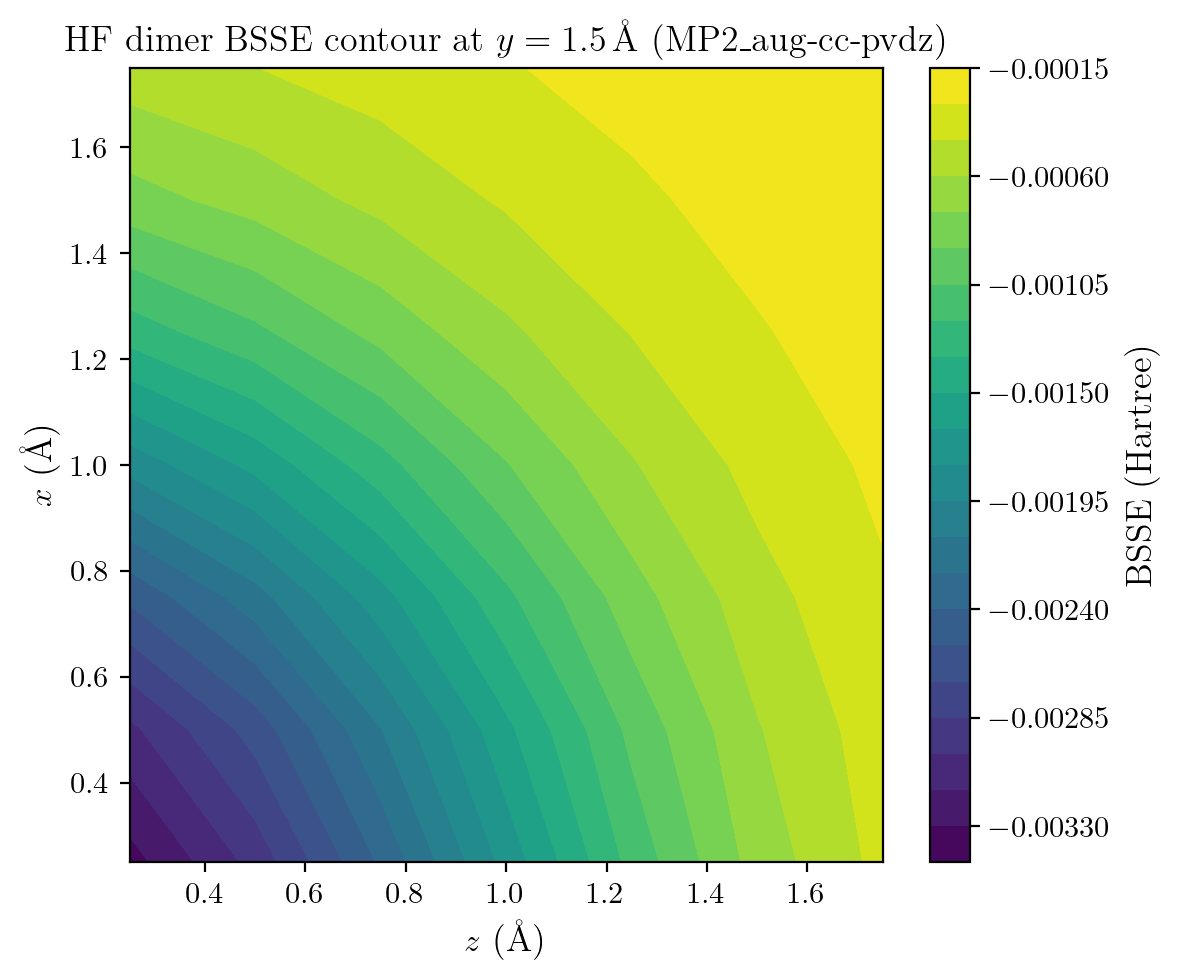
\includegraphics[width=\textwidth]{figures/dimer/HF_dimer/HF_trnl_contour_1.5_MP2.png}
        \caption{MP2 corr., $y = \SI{1.5}{\angstrom}$}
    \end{subfigure}
    \hfill
    \begin{subfigure}[b]{0.32\textwidth}
        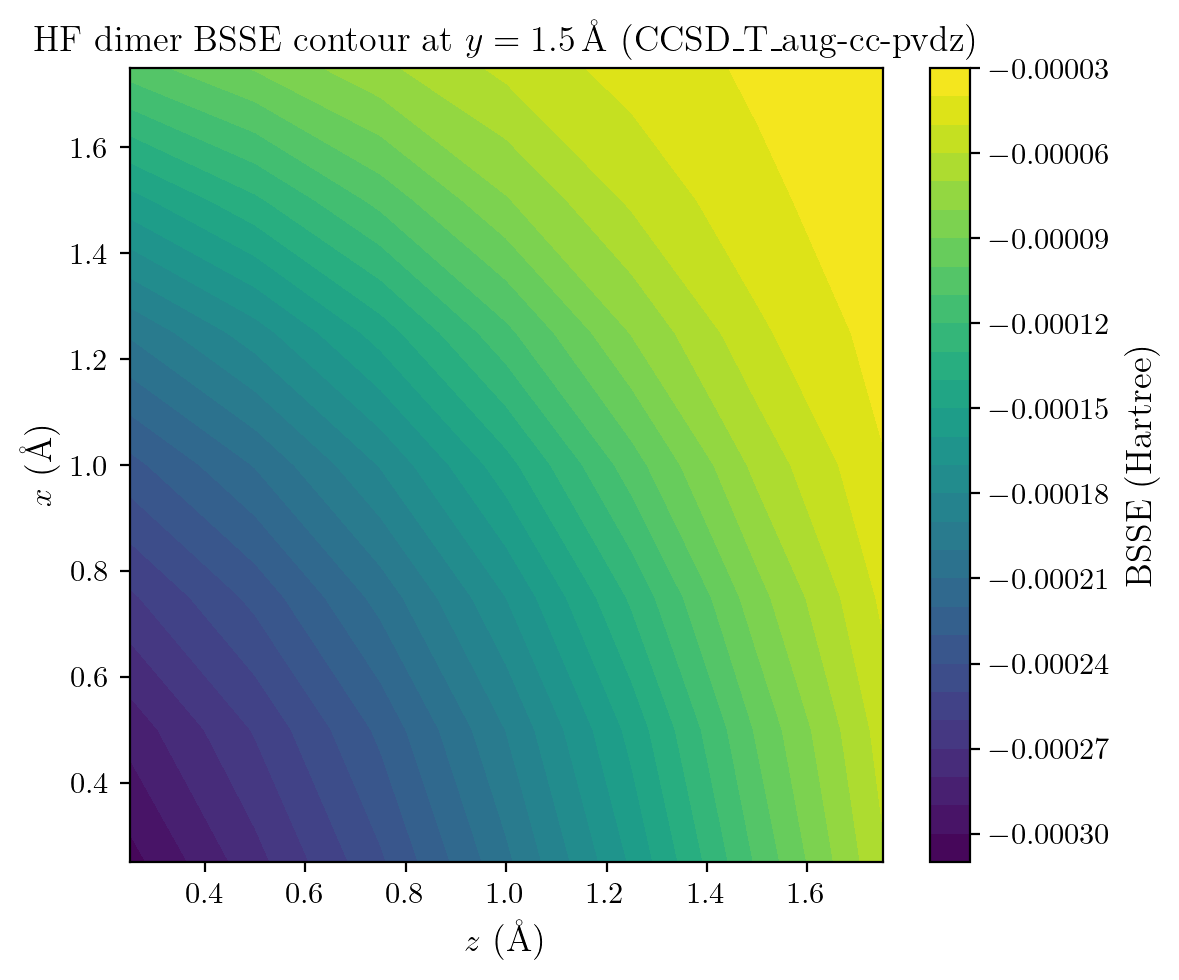
\includegraphics[width=\textwidth]{figures/dimer/HF_dimer/HF_trnl_contour_1.5_CCSD_T.png}
        \caption{CCSD(T) corr., $y = \SI{1.5}{\angstrom}$}
    \end{subfigure}

    \vspace{0.8em}

    \begin{subfigure}[b]{0.32\textwidth}
        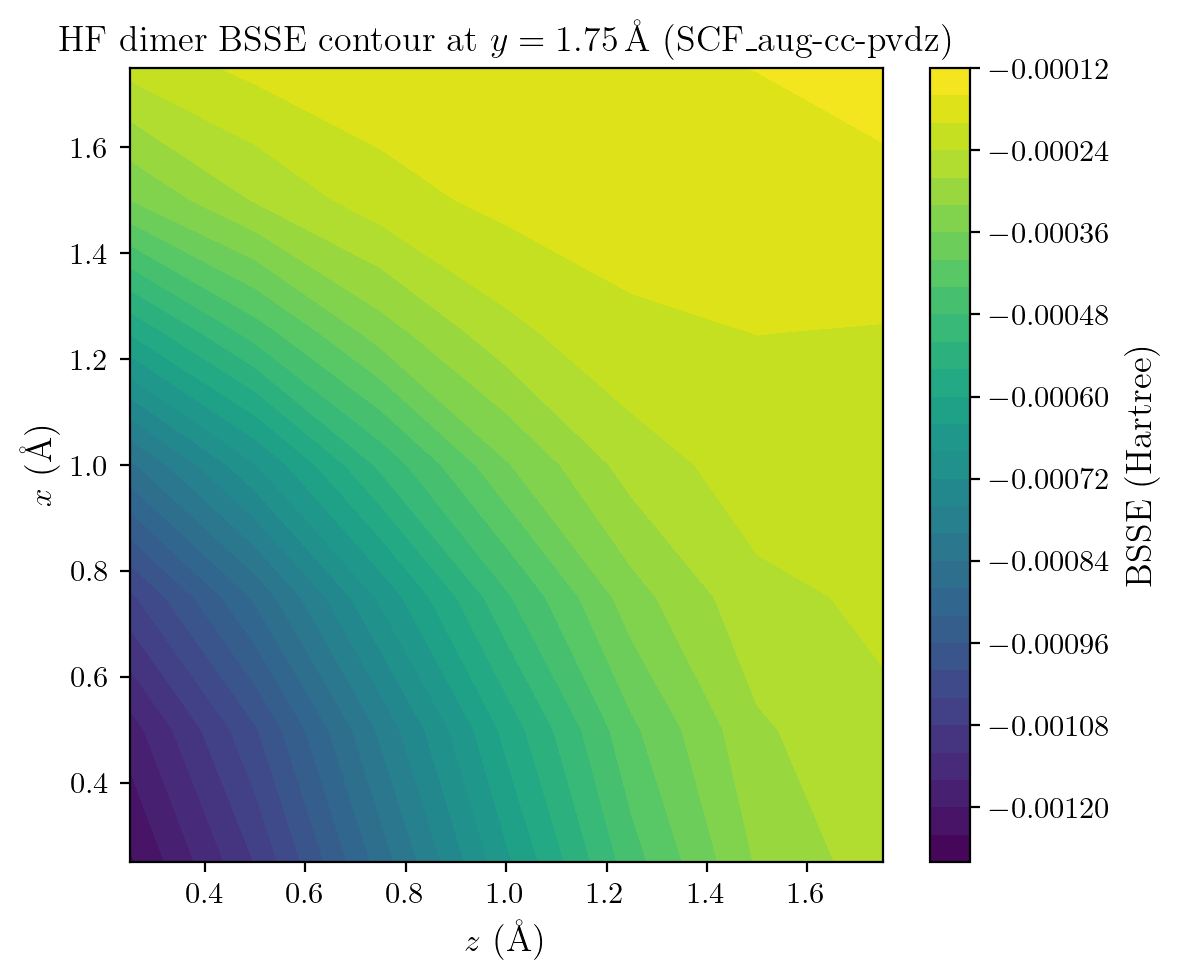
\includegraphics[width=\textwidth]{figures/dimer/HF_dimer/HF_trnl_contour_1.75_SCF.png}
        \caption{SCF, $y = \SI{1.75}{\angstrom}$}
    \end{subfigure}
    \hfill
    \begin{subfigure}[b]{0.32\textwidth}
        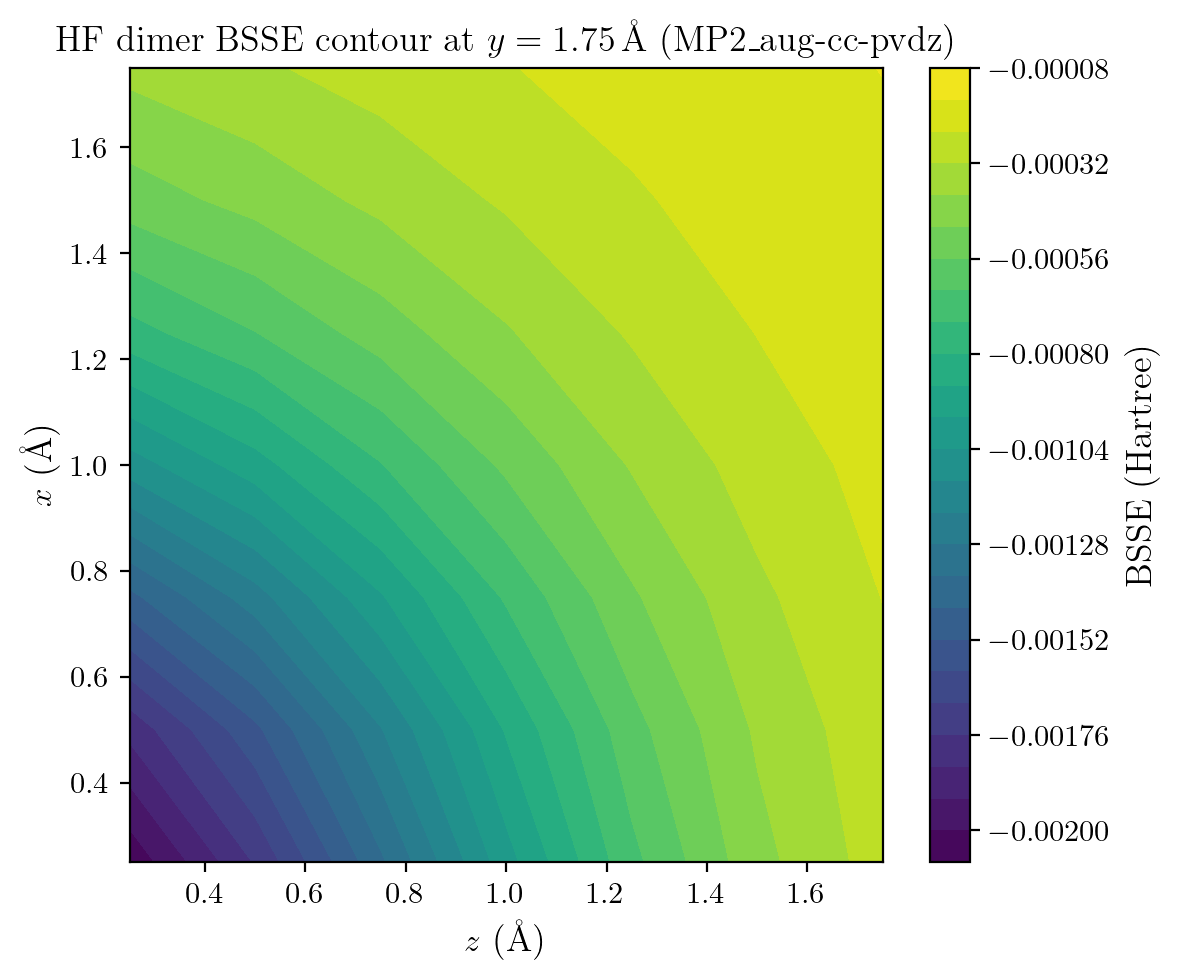
\includegraphics[width=\textwidth]{figures/dimer/HF_dimer/HF_trnl_contour_1.75_MP2.png}
        \caption{MP2 corr., $y = \SI{1.75}{\angstrom}$}
    \end{subfigure}
    \hfill
    \begin{subfigure}[b]{0.32\textwidth}
        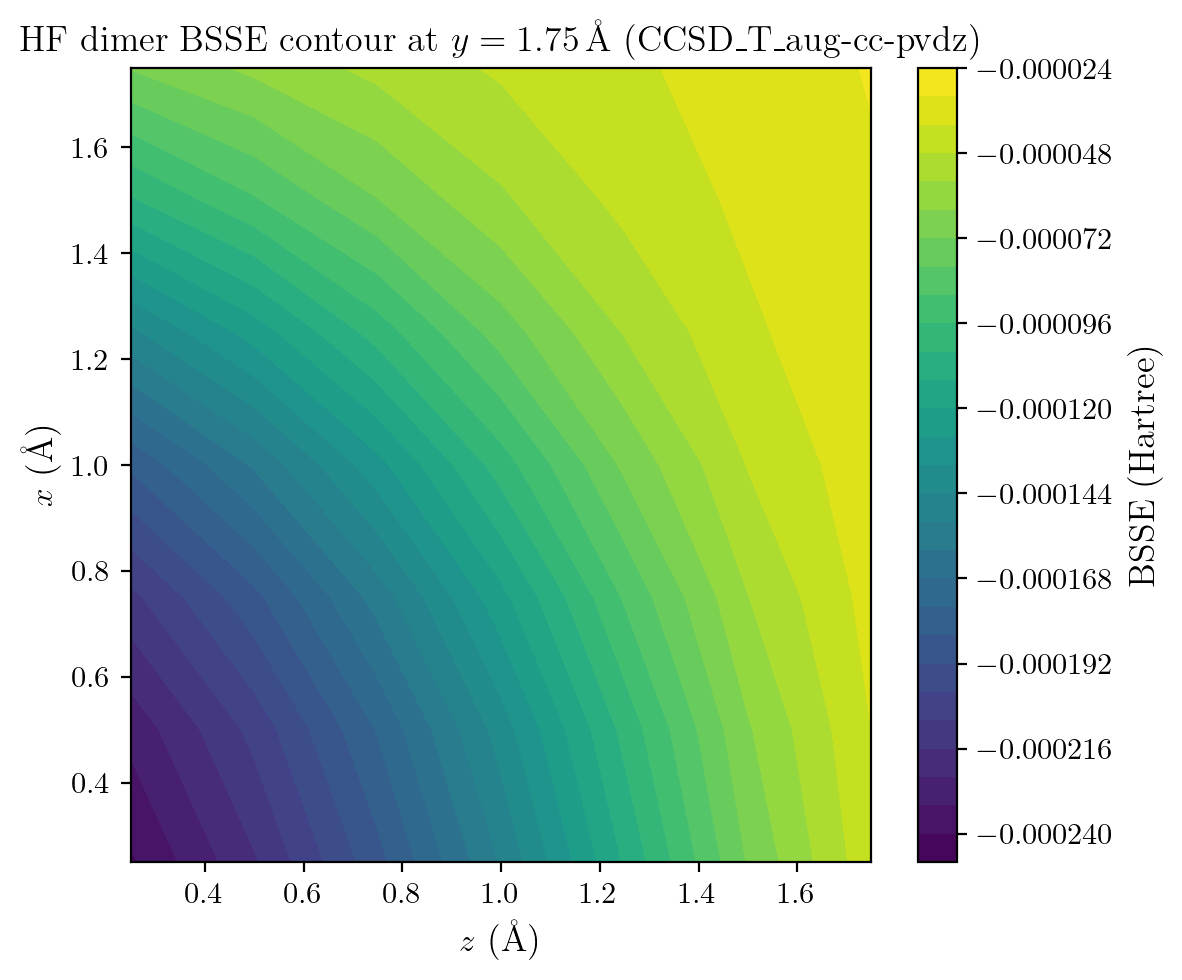
\includegraphics[width=\textwidth]{figures/dimer/HF_dimer/HF_trnl_contour_1.75_CCSD_T.png}
        \caption{CCSD(T) corr., $y = \SI{1.75}{\angstrom}$}
    \end{subfigure}

    \caption{BSSE contour plots for the HF dimer translational scan at
    fixed $y = 1.5$ and \SI{1.75}{\angstrom}. Axes correspond to the
    in-plane F--F displacement components $(x, z)$ in \AA. Contour
    levels represent the BSSE in Hartree. The MP2 and CCSD(T) labels
    refer to the correlation energy components relative to SCF and MP2,
    respectively. At $y = \SI{1.5}{\angstrom}$ all three methods show
    nearly circular contours; at $y = \SI{1.75}{\angstrom}$ the SCF
    contours develop a visible asymmetry between the $x$ and $z$
    directions, reflecting the polar and heteronuclear character of
    the HF monomer.}
    \label{fig:hf_trnl_contours}
\end{figure}

At $y = \SI{1.5}{\angstrom}$, all three methods show nearly circular
contour arcs, consistent with the behavior observed for Ne and
\ce{H2O}. At $y = \SI{1.75}{\angstrom}$, the MP2 and CCSD(T)
contours remain circular, but the SCF contours develop a visible
asymmetry between the $x$ and $z$ directions.

%----------------------------------------------------------------------
% TODO: pending PI discussion — physical interpretation of SCF asymmetry
%-----------------------------------------------------------------------
% This asymmetry is a physical effect, not a numerical artifact. The
% computational grid was verified to be perfectly symmetric (a $7 \times
% 7$ grid with identical $x$ and $z$ ranges), ruling out any grid
% artifact. The origin of the asymmetry lies in the heteronuclear nature
% of HF: unlike Ne (spherically symmetric) and \ce{H2O} (which has a
% $C_{2v}$ symmetry axis), HF has distinct H and F ends. At
% $y = \SI{1.75}{\angstrom}$ the in-plane displacement components become
% comparable to the HF bond length (\SI{0.924}{\angstrom}), making the
% orientation of H vs F relative to the displacement direction
% observable in the SCF BSSE. The fact that this asymmetry appears at
% the SCF level but not in the MP2 and CCSD(T) correlation components
% suggests it arises from the anisotropy of the SCF electron density of
% the HF monomer rather than from correlation effects.

\clearpage
% ----------------------------------------------------------------------
\subsection{Rotational--Radial Scan Results}
% ----------------------------------------------------------------------

Figure~\ref{fig:hf_rot_bsse_vs_R} shows $|\text{BSSE}|$ as a function
of $R$ for 9 representative orientations, with SCF, MP2 correlation,
and CCSD(T) correlation components overlaid on each panel.

\begin{figure}[H]
    \centering
    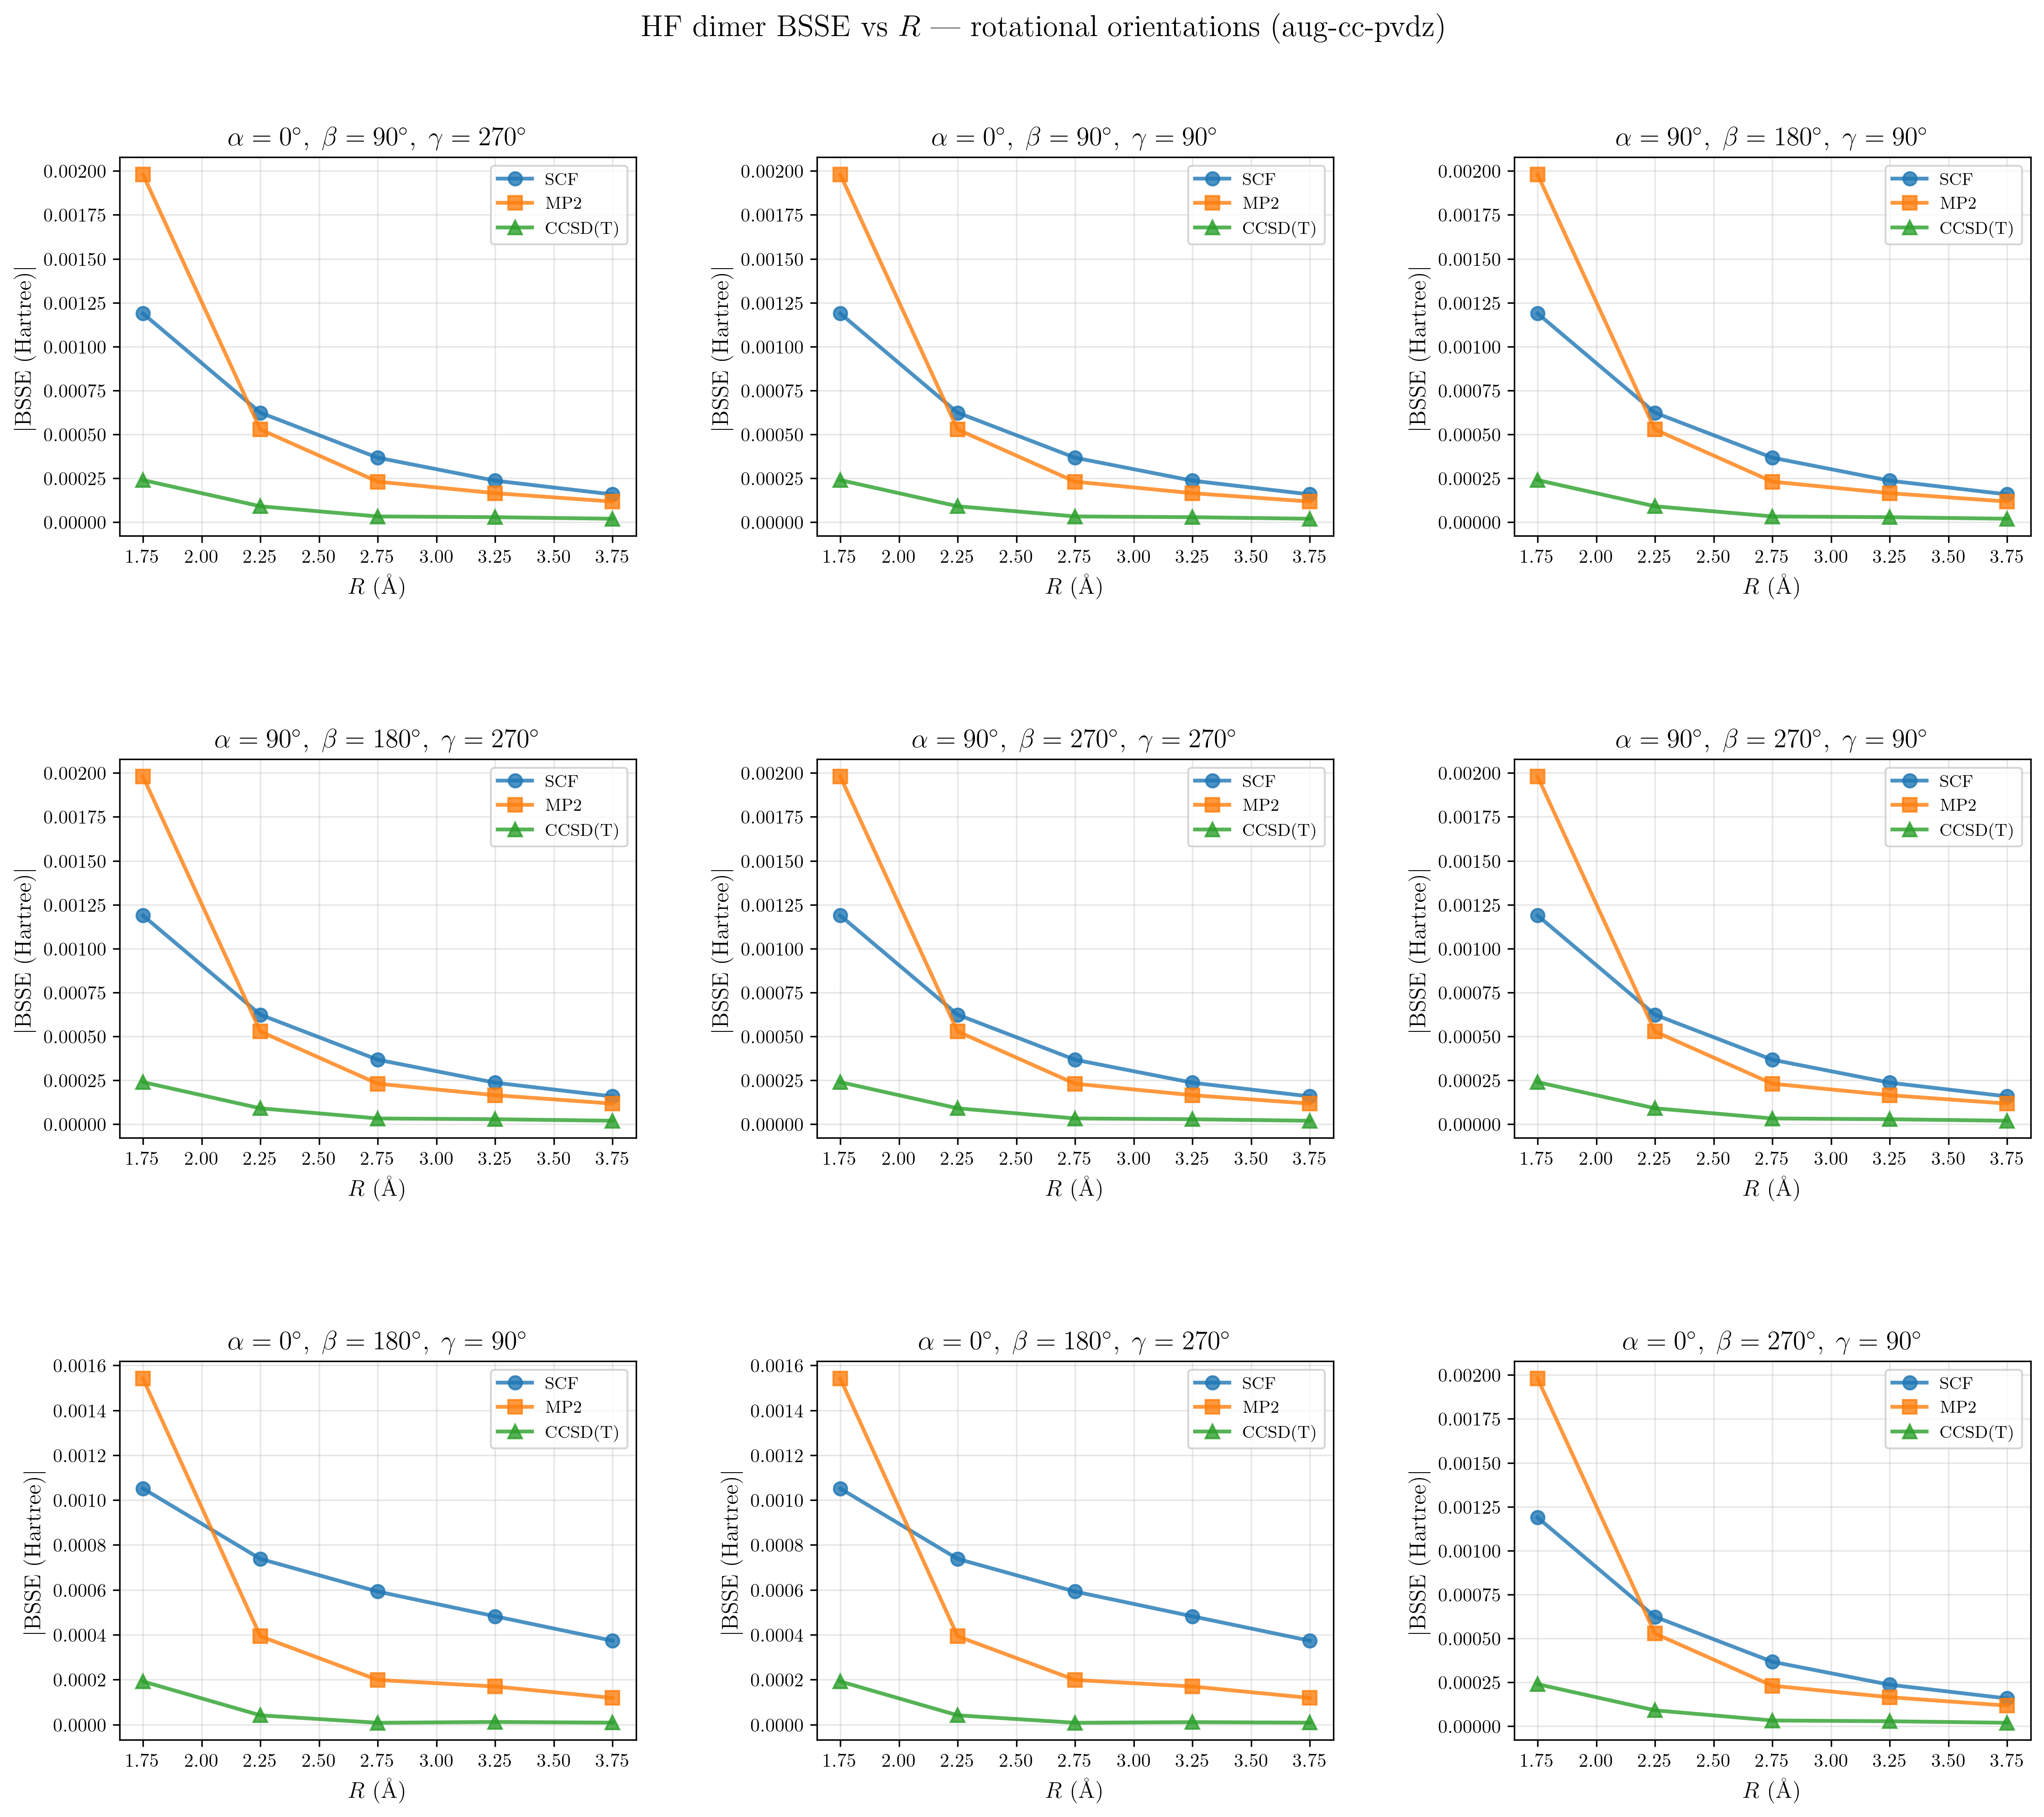
\includegraphics[scale=0.38]{figures/dimer/HF_dimer/HF_rot_vs_R_SCFMP2CCSD_T.png}
    \caption{$|\text{BSSE}|$ vs F--F separation $R$ for 9
    representative rotational orientations of the HF dimer at the
    aug-cc-pVDZ level. Each panel corresponds to a distinct set of
    Euler angles $(\alpha, \beta, \gamma)$ as labeled; all orientations
    have $\alpha = 90.0°$. Blue circles: SCF contribution; orange
    squares: MP2 correlation component
    ($E_\text{MP2} - E_\text{SCF}$); green triangles: CCSD(T)
    correlation component ($E_{\text{CCSD(T)}} - E_\text{MP2}$).
    All three components decay monotonically with $R$ and show
    consistent behavior across orientations, confirming weak
    orientation dependence of HF dimer BSSE despite the asymmetry
    observed in the SCF translational contours.}
    \label{fig:hf_rot_bsse_vs_R}
\end{figure}

\clearpage

All 9 orientations show identical monotonic decay of $|\text{BSSE}|$
with $R$ across all three methods. The shape and magnitude of the
curves are consistent across the sampled $(\alpha, \beta, \gamma)$
values, confirming that the orientation dependence of HF dimer BSSE
is weak overall --- the asymmetry visible in the SCF translational
contour at $y = \SI{1.75}{\angstrom}$ does not translate into
significant variation across rotational orientations at fixed $R$.
As in the Ne and \ce{H2O} dimers, the MP2 correlation component is
the dominant contribution at all distances sampled.



% ----------------------------------------------------------------------
\subsection{Key Findings}
% ----------------------------------------------------------------------

\begin{finding_box}
\textbf{HF dimer BSSE is primarily governed by F--F distance, with a
physically real short-range asymmetry.}
The translational contour plots show nearly circular arcs at
$y = \SI{1.5}{\angstrom}$, consistent with Ne and \ce{H2O}. At
$y = \SI{1.75}{\angstrom}$, the SCF contours develop a visible
asymmetry between the $x$ and $z$ directions. This asymmetry is
confirmed to be a physical effect of the heteronuclear HF geometry:
at short range, when the displacement components are comparable to
the HF bond length, the orientation of H vs F becomes observable in
the SCF BSSE. The MP2 and CCSD(T) correlation components remain
circular at both $y$ values.
\end{finding_box}

\begin{finding_box}
\textbf{Orientation dependence of HF dimer BSSE is weak overall.}
Despite the asymmetry in the SCF translational contours, the
rotational--radial scan shows that $|\text{BSSE}|$ vs $R$ curves are
consistent across all 28 eligible orientations. The dominant
contribution across all distances and orientations is the MP2
correlation component, with a small CCSD(T) increment, mirroring the
behavior seen in the Ne and \ce{H2O} dimers.
\end{finding_box}

\clearpage

%-----------------------------------------------------------------------
% Chapter 4 — Trimer: Setup and Infrastructure
%-----------------------------------------------------------------------
%\chapter{\ce{H2O} Trimer: Data Pipeline}
%% trimer_setup.tex — Chapter 4: Trimer BSSE Analysis — Setup and Geometry
% Project: rmrresearch/bsse_db | Branch: fcuantico
% Molecules: H2O (complete), Ne (complete), HF (complete)

% ======================================================================
\section{\ce{H2O} Trimer}
% ======================================================================

% ----------------------------------------------------------------------
\subsection{Overview}
% ----------------------------------------------------------------------

The \ce{H2O} trimer extends the dimer analysis to a three-body system.
Five O--O distances are studied: $R = 2.75$, $3.0$, $3.25$, $3.5$,
and \SI{3.75}{\angstrom}. All calculations were performed at the SCF,
MP2, and CCSD(T) levels using the aug-cc-pVDZ basis
set~\cite{dunning1989,kendall1992} with the NWChem quantum chemistry
package~\cite{nwchem2020}. The many-body BSSE decomposition follows
the VMFC scheme~\cite{valiron1997}.

% ----------------------------------------------------------------------
\subsection{Geometry}
% ----------------------------------------------------------------------

The three \ce{H2O} monomers, labeled A, B, and C, are arranged in a
planar equilateral triangle with all atoms in the $xy$ plane ($z = 0$).
Within each monomer the O--H bond lengths and H--O--H angle are held
fixed at their equilibrium values, identical to those used in the dimer
calculations. Table~\ref{tab:h2o_trimer_geometry} lists the Cartesian
coordinates at $R = \SI{2.75}{\angstrom}$, the shortest O--O distance
in the dataset. For the remaining configurations the triangle is
uniformly expanded while preserving the equilateral arrangement and
the monomer internal geometry.

\begin{table}[!ht]
    \centering
    \caption{Cartesian coordinates of the \ce{H2O} trimer at
    $R = \SI{2.75}{\angstrom}$ (aug-cc-pVDZ, NWChem convention).
    Atom labels: A = monomer~A (oxygen at origin), B = monomer~B
    (oxygen at upper vertex), C = monomer~C (oxygen at right vertex).
    All coordinates in \AA.}
    \label{tab:h2o_trimer_geometry}
    \begin{tabular}{lcccc}
        \toprule
        Atom & Monomer & $x$ (\AA) & $y$ (\AA) & $z$ (\AA) \\
        \midrule
        O & A & $-0.15219$ & $-0.00116$ & $0.00000$ \\
        H & A & $ 0.43777$ & $-0.76611$ & $0.00000$ \\
        H & A & $ 0.44760$ & $ 0.75608$ & $0.00000$ \\
        O & B & $ 1.47281$ & $ 2.81342$ & $0.00000$ \\
        H & B & $ 2.06277$ & $ 2.04847$ & $0.00000$ \\
        H & B & $ 2.07260$ & $ 3.57066$ & $0.00000$ \\
        O & C & $ 3.09781$ & $-0.00116$ & $0.00000$ \\
        H & C & $ 3.68777$ & $-0.76611$ & $0.00000$ \\
        H & C & $ 3.69760$ & $ 0.75608$ & $0.00000$ \\
        \bottomrule
    \end{tabular}
\end{table}



% TODO: move this table to theory.tex when that chapter is written
\subsection{VMFC File Keys}
% ----------------------------------------------------------------------

The VMFC scheme for a three-monomer system (A, B, C) requires a total
of 19 distinct NWChem calculations per configuration. Each calculation
is identified by a \textit{file key} of the form \texttt{real\_basis},
where \texttt{real} denotes the monomer(s) treated as real atoms and
\texttt{basis} denotes the set of monomers contributing basis
functions. Table~\ref{tab:h2o_trimer_filekeys} lists all 19 file keys
and their physical meaning.

\begin{table}[!ht]
    \centering
    \caption{The 19 VMFC file keys for the \ce{H2O} trimer. The
    \texttt{real\_basis} naming convention follows the folder structure
    in \texttt{bsse\_db}: \texttt{real} = real atoms, \texttt{basis} =
    basis set used (own + ghost atoms). Keys with identical monomers
    (e.g.\ \texttt{B\_B} and \texttt{A\_A}) are verified numerically
    to confirm monomer equivalence.}
    \label{tab:h2o_trimer_filekeys}
    \small
    \begin{tabular}{lll}
        \toprule
        File key & Real atoms & Basis set \\
        \midrule
        \texttt{A\_A}    & A     & A only \\
        \texttt{B\_B}    & B     & B only \\
        \texttt{C\_C}    & C     & C only \\
        \texttt{AB\_AB}  & A, B  & AB \\
        \texttt{AC\_AC}  & A, C  & AC \\
        \texttt{BC\_BC}  & B, C  & BC \\
        \texttt{ABC\_ABC}& A, B, C & ABC (full trimer) \\
        \texttt{A\_AB}   & A     & AB (B as ghost) \\
        \texttt{B\_AB}   & B     & AB (A as ghost) \\
        \texttt{A\_AC}   & A     & AC (C as ghost) \\
        \texttt{C\_AC}   & C     & AC (A as ghost) \\
        \texttt{B\_BC}   & B     & BC (C as ghost) \\
        \texttt{C\_BC}   & C     & BC (B as ghost) \\
        \texttt{A\_ABC}  & A     & ABC (B, C as ghosts) \\
        \texttt{B\_ABC}  & B     & ABC (A, C as ghosts) \\
        \texttt{C\_ABC}  & C     & ABC (A, B as ghosts) \\
        \texttt{AB\_ABC} & A, B  & ABC (C as ghost) \\
        \texttt{AC\_ABC} & A, C  & ABC (B as ghost) \\
        \texttt{BC\_ABC} & B, C  & ABC (A as ghost) \\
        \bottomrule
    \end{tabular}
\end{table}

The 19 file keys divide naturally into four groups by the size of the
basis set used: the three monomer-in-own-basis calculations
(\texttt{A\_A}, \texttt{B\_B}, \texttt{C\_C}), the six
monomer-in-dimer-basis calculations (\texttt{A\_AB}, \texttt{B\_AB},
etc.), the three monomer-in-trimer-basis calculations
(\texttt{A\_ABC}, \texttt{B\_ABC}, \texttt{C\_ABC}), and the three
dimer-in-trimer-basis calculations (\texttt{AB\_ABC}, \texttt{AC\_ABC},
\texttt{BC\_ABC}). Together these calculations provide all the
ingredients needed to evaluate both FORM~I and FORM~II of the VMFC
BSSE decomposition.

% ----------------------------------------------------------------------
\subsection{Configuration Summary}
% ----------------------------------------------------------------------

Table~\ref{tab:h2o_trimer_configs} summarizes the five \ce{H2O} trimer
configurations studied in this work.

\begin{table}[!ht]
    \centering
    \caption{Summary of the five \ce{H2O} trimer configurations.
    All configurations use the aug-cc-pVDZ basis set and were computed
    at the SCF, MP2, and CCSD(T) levels of theory.}
    \label{tab:h2o_trimer_configs}
    \begin{tabular}{ccc}
        \toprule
        Configuration & O--O Distance (\AA) & File key count \\
        \midrule
        0 & 2.75 & 19 \\
        1 & 3.00 & 19 \\
        2 & 3.25 & 19 \\
        3 & 3.50 & 19 \\
        4 & 3.75 & 19 \\
        \bottomrule
    \end{tabular}
\end{table}

% ======================================================================
\section{Ne Trimer}
% ======================================================================

% ----------------------------------------------------------------------
\subsection{Overview}
% ----------------------------------------------------------------------

The Ne trimer extends the dimer analysis to a three-body system of
rare-gas atoms. Ten Ne--Ne distances are studied: $R = 1.5$, $1.75$,
$2.0$, $2.25$, $2.5$, $2.75$, $3.0$, $3.25$, $3.5$, and
\SI{3.75}{\angstrom}. All calculations were performed at the SCF, MP2,
and CCSD(T) levels using the aug-cc-pVDZ basis
set~\cite{dunning1989,kendall1992} with the NWChem quantum chemistry
package~\cite{nwchem2020}. The many-body BSSE decomposition follows
the VMFC scheme~\cite{valiron1997}.

% ----------------------------------------------------------------------
\subsection{Geometry}
% ----------------------------------------------------------------------

The three Ne atoms, labeled A, B, and C, are arranged in a planar
equilateral triangle with all atoms in the $xy$ plane ($z = 0$).
Table~\ref{tab:ne_trimer_geometry} lists the Cartesian coordinates at
$R = \SI{1.5}{\angstrom}$, the shortest Ne--Ne distance in the dataset.
For the remaining configurations the triangle is uniformly expanded
while preserving the equilateral arrangement. The three pairwise
distances AB, AC, and BC are identical by construction at every
configuration.

\begin{table}[!ht]
    \centering
    \caption{Cartesian coordinates of the Ne trimer at
    $R = \SI{1.5}{\angstrom}$ (aug-cc-pVDZ, NWChem convention).
    Atom labels: A = monomer~A (at origin), B = monomer~B
    (upper vertex), C = monomer~C (right vertex).
    All coordinates in \AA.}
    \label{tab:ne_trimer_geometry}
    \begin{tabular}{lcccc}
        \toprule
        Atom & Monomer & $x$ (\AA) & $y$ (\AA) & $z$ (\AA) \\
        \midrule
        Ne & A & $0.00000000$ & $0.00000000$ & $0.00000000$ \\
        Ne & B & $0.75000000$ & $1.29903811$ & $0.00000000$ \\
        Ne & C & $1.50000000$ & $0.00000000$ & $0.00000000$ \\
        \bottomrule
    \end{tabular}
\end{table}

Because all three Ne monomers are identical, the three monomer
energies are numerically equal: $E_\text{A}(\text{A}) =
E_\text{B}(\text{B}) = E_\text{C}(\text{C})$ at every level of theory
and every configuration. This identity is verified numerically in the
pipeline and used to confirm the integrity of the parsed data.

% ----------------------------------------------------------------------
\subsection{Configuration Summary}
% ----------------------------------------------------------------------

Table~\ref{tab:ne_trimer_configs} summarizes the ten Ne trimer
configurations studied in this work.

\begin{table}[!ht]
    \centering
    \caption{Summary of the ten Ne trimer configurations.
    All configurations use the aug-cc-pVDZ basis set and were computed
    at the SCF, MP2, and CCSD(T) levels of theory.}
    \label{tab:ne_trimer_configs}
    \begin{tabular}{ccc}
        \toprule
        Configuration & Ne--Ne Distance (\AA) & File key count \\
        \midrule
        0 & 1.50 & 19 \\
        1 & 1.75 & 19 \\
        2 & 2.00 & 19 \\
        3 & 2.25 & 19 \\
        4 & 2.50 & 19 \\
        5 & 2.75 & 19 \\
        6 & 3.00 & 19 \\
        7 & 3.25 & 19 \\
        8 & 3.50 & 19 \\
        9 & 3.75 & 19 \\
        \bottomrule
    \end{tabular}
\end{table}

% ======================================================================
\section{HF Trimer}
% ======================================================================

% ----------------------------------------------------------------------
\subsection{Overview}
% ----------------------------------------------------------------------

The HF trimer extends the dimer analysis to a three-body system of
hydrogen fluoride molecules. Seven F--F distances are studied:
$R = 1.5$, $1.75$, $2.0$, $2.25$, $2.5$, $2.75$, and
\SI{3.0}{\angstrom}. All calculations were performed at the SCF, MP2,
and CCSD(T) levels using the aug-cc-pVDZ basis
set~\cite{dunning1989,kendall1992} with the NWChem quantum chemistry
package~\cite{nwchem2020}. The many-body BSSE decomposition follows
the VMFC scheme~\cite{valiron1997}.

% ----------------------------------------------------------------------
\subsection{Geometry}
% ----------------------------------------------------------------------

The three HF monomers, labeled A, B, and C, are arranged so that the
three fluorine atoms form a planar equilateral triangle in the $xy$
plane ($z = 0$), with the hydrogen atom of each monomer displaced
along the negative $z$ direction. Within each monomer the H--F bond
length is held fixed. Table~\ref{tab:hf_trimer_geometry} lists the
Cartesian coordinates at $R = \SI{1.5}{\angstrom}$, the shortest F--F
distance in the dataset. For the remaining configurations the
fluorine triangle is uniformly expanded while preserving the
equilateral arrangement and the monomer internal geometry.

\begin{table}[!ht]
    \centering
    \caption{Cartesian coordinates of the HF trimer at
    $R = \SI{1.5}{\angstrom}$ (aug-cc-pVDZ, NWChem convention).
    Atom labels: A = monomer~A (F at origin), B = monomer~B
    (F at upper vertex), C = monomer~C (F at right vertex).
    The three F atoms lie in the $z = 0$ plane; the H atoms are
    displaced to $z = -0.924$~\AA. All coordinates in \AA.}
    \label{tab:hf_trimer_geometry}
    \begin{tabular}{lcccc}
        \toprule
        Atom & Monomer & $x$ (\AA) & $y$ (\AA) & $z$ (\AA) \\
        \midrule
        F & A & $0.00000000$ & $0.00000000$ & $ 0.00000000$ \\
        H & A & $0.00000000$ & $0.00000000$ & $-0.92400000$ \\
        F & B & $0.75000000$ & $1.29903811$ & $ 0.00000000$ \\
        H & B & $0.75000000$ & $1.29903811$ & $-0.92400000$ \\
        F & C & $1.50000000$ & $0.00000000$ & $ 0.00000000$ \\
        H & C & $1.50000000$ & $0.00000000$ & $-0.92400000$ \\
        \bottomrule
    \end{tabular}
\end{table}

Although the HF monomer is a diatomic and the three monomers are
individually equivalent, the H atoms point out of the fluorine plane,
breaking the in-plane $C_{3v}$ symmetry present in the Ne trimer.
Nevertheless, the three F--F pairwise distances AB, AC, and BC remain
identical by construction at every configuration, and the three
monomer energies are numerically equal:
$E_\text{A}(\text{A}) = E_\text{B}(\text{B}) = E_\text{C}(\text{C})$
at every level of theory.

% ----------------------------------------------------------------------
\subsection{Configuration Summary}
% ----------------------------------------------------------------------

Table~\ref{tab:hf_trimer_configs} summarizes the seven HF trimer
configurations studied in this work.

\begin{table}[!ht]
    \centering
    \caption{Summary of the seven HF trimer configurations.
    All configurations use the aug-cc-pVDZ basis set and were computed
    at the SCF, MP2, and CCSD(T) levels of theory.}
    \label{tab:hf_trimer_configs}
    \begin{tabular}{ccc}
        \toprule
        Configuration & F--F Distance (\AA) & File key count \\
        \midrule
        0 & 1.50 & 19 \\
        1 & 1.75 & 19 \\
        2 & 2.00 & 19 \\
        3 & 2.25 & 19 \\
        4 & 2.50 & 19 \\
        5 & 2.75 & 19 \\
        6 & 3.00 & 19 \\
        \bottomrule
    \end{tabular}
\end{table}

%-----------------------------------------------------------------------
% Chapter 5 — Trimer: BSSE Decomposition
%-----------------------------------------------------------------------
% \chapter{\ce{H2O} Trimer: BSSE Decomposition}
% % trimer_bsse.tex — Chapter 4: Trimer BSSE Analysis — BSSE Results
% Project: rmrresearch/bsse_db | Branch: fcuantico
% Molecules: H2O (complete), Ne (complete), HF (complete)

% ======================================================================
\section{\ce{H2O} Trimer BSSE Results}
% ======================================================================

% ----------------------------------------------------------------------
\subsection{Total BSSE vs O--O Distance}
% ----------------------------------------------------------------------

Figure~\ref{fig:h2o_trimer_plot1} shows the total BSSE as a function
of O--O distance $R$ for all three levels of theory.

\begin{figure}[!ht]
    \centering
    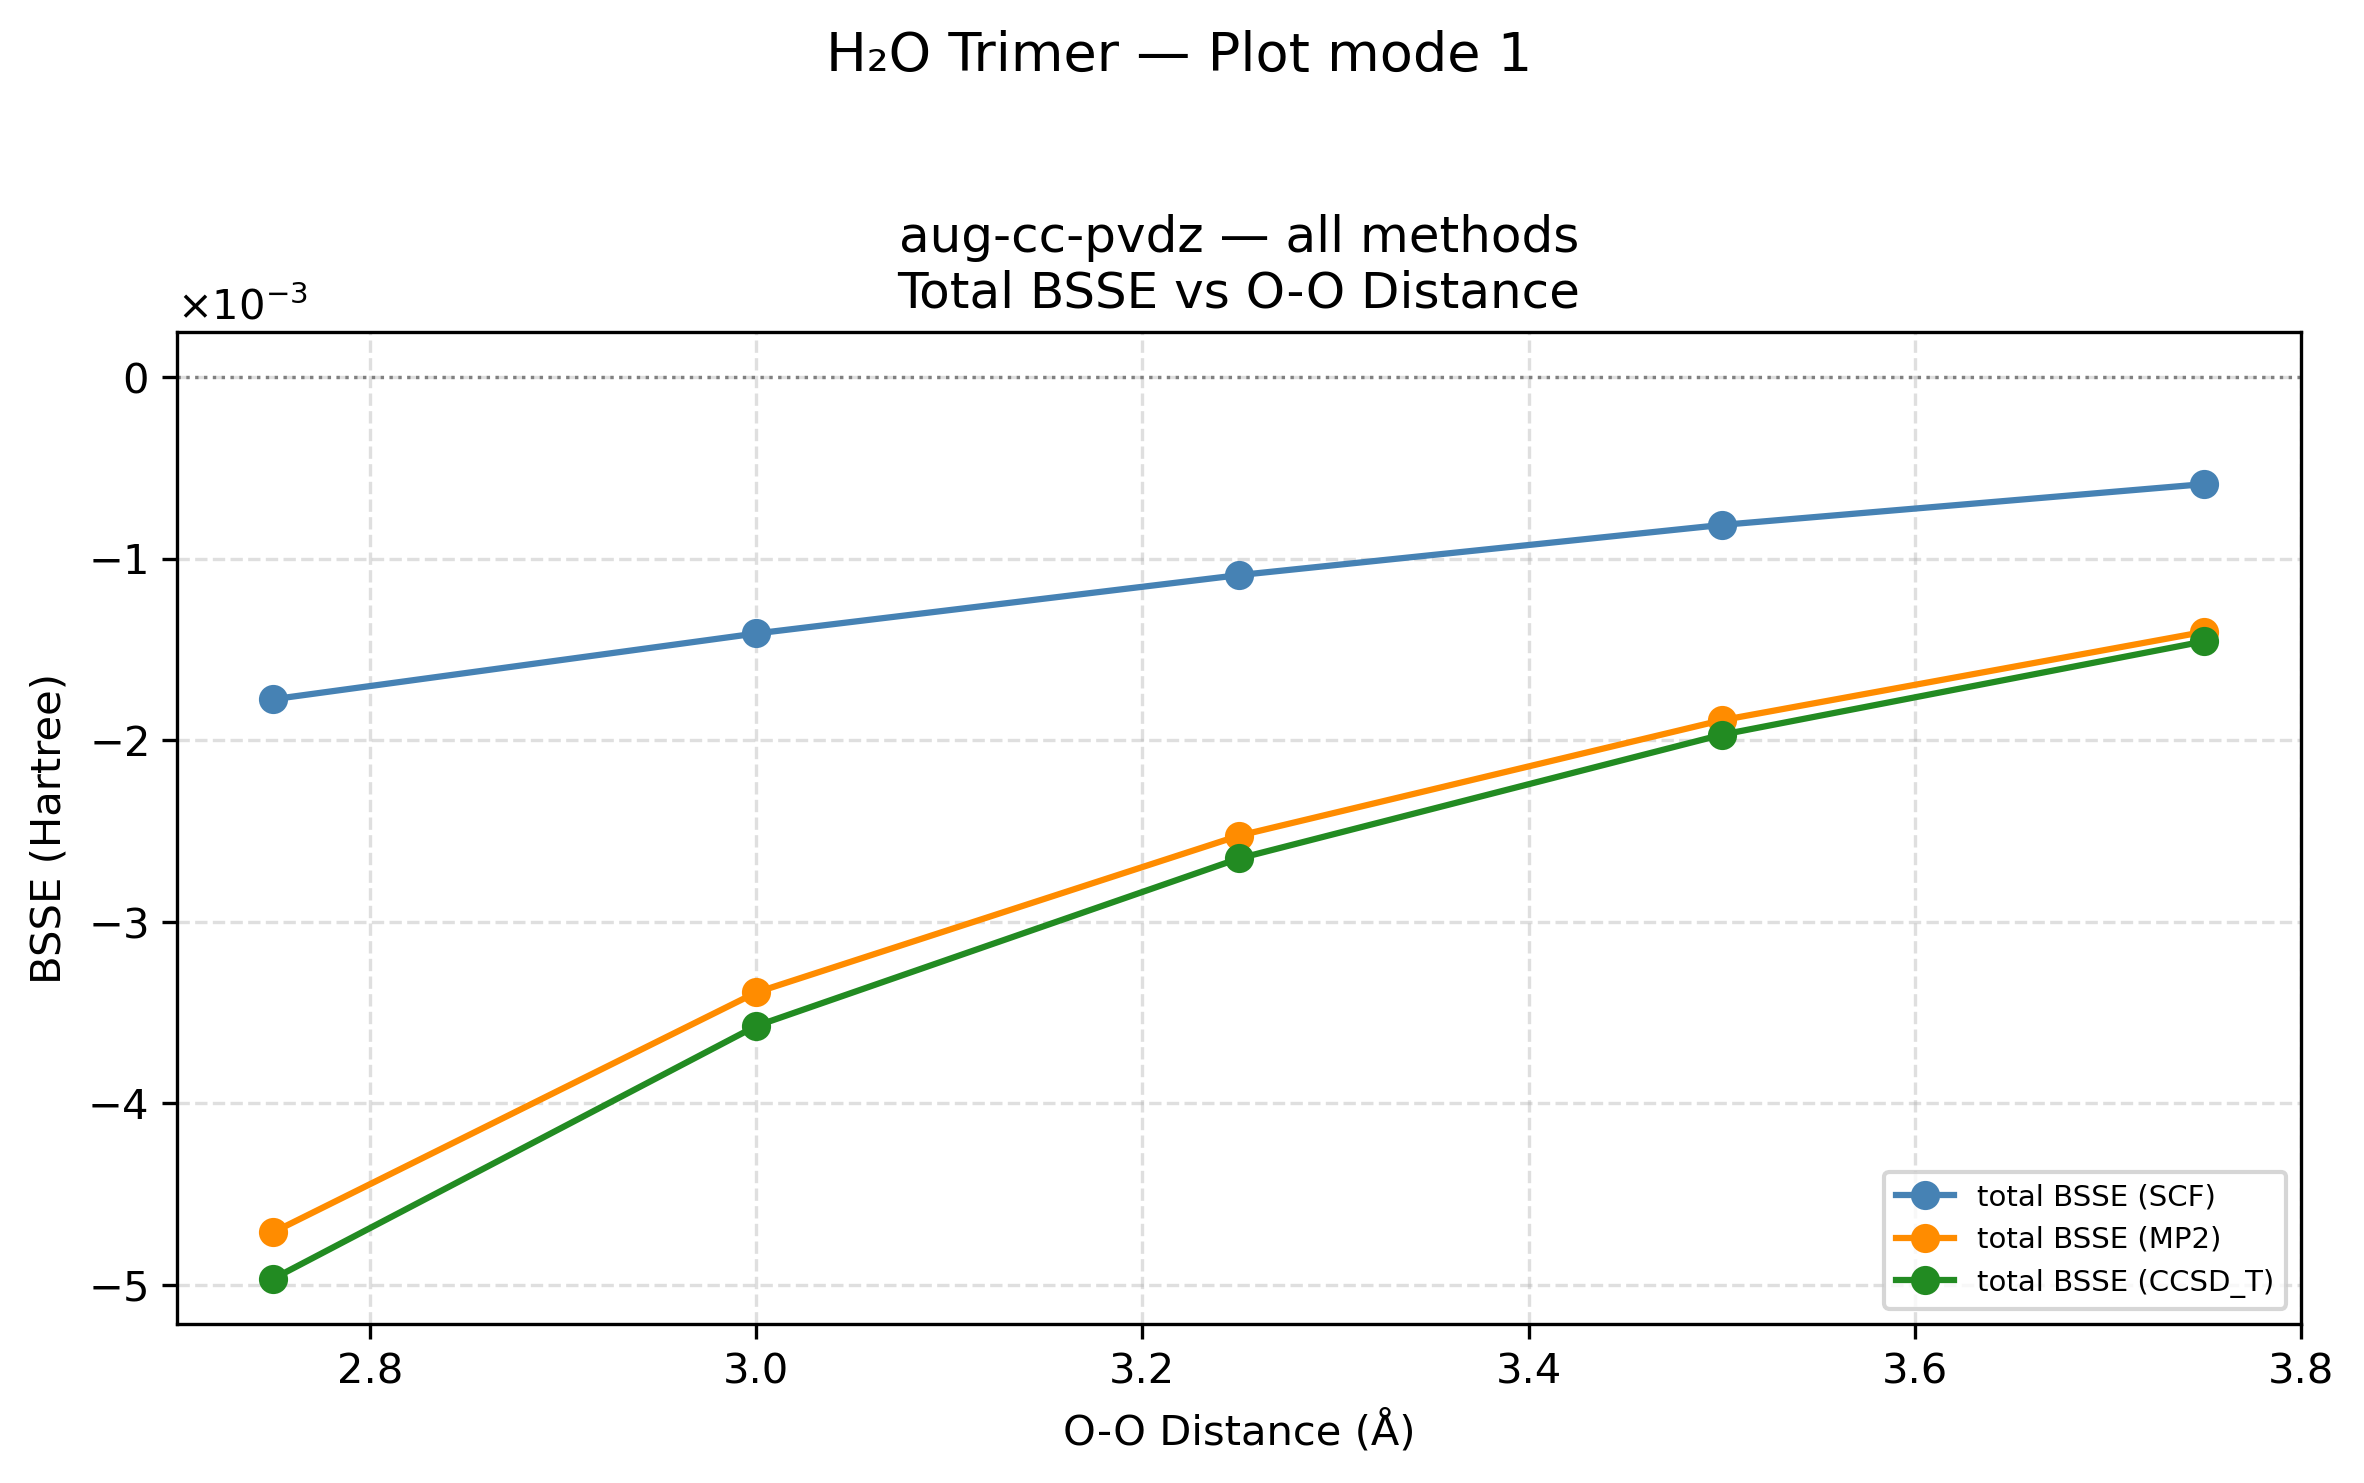
\includegraphics[width=1.0\textwidth]{figures/trimer/H2O_trimer/plot1_all_aug-cc-pvdz.png}
    \caption{Total BSSE vs O--O distance $R$ for the \ce{H2O} trimer
    at the aug-cc-pVDZ level. Blue circles: SCF; orange squares: MP2;
    green triangles: CCSD(T). All values are in Hartree. All three
    curves approach zero monotonically with increasing $R$. The MP2
    and CCSD(T) curves are close in magnitude and significantly larger
    than the SCF contribution at all distances sampled.}
    \label{fig:h2o_trimer_plot1}
\end{figure}

All three curves are negative and approach zero monotonically with
increasing $R$, consistent with the expected reduction of basis set
overlap at larger separations. At the shortest distance ($R = \SI{2.75}{\angstrom}$) the
total BSSE values are approximately $-1.8 \times 10^{-3}$~Ha (SCF),
$-4.7 \times 10^{-3}$~Ha (MP2), and $-5.0 \times 10^{-3}$~Ha
(CCSD(T)). The MP2 and CCSD(T) curves are close throughout the range,
while the SCF contribution is smaller in magnitude by roughly a factor
of three.

% ----------------------------------------------------------------------
\subsection{Two-Body and Three-Body Decomposition}
% ----------------------------------------------------------------------

Figure~\ref{fig:h2o_trimer_plot2} separates the total BSSE into its
two-body ($\theta^{(2)}$) and three-body ($\theta^{(3)}$) components
for each level of theory.

\begin{figure}[!ht]
    \centering
    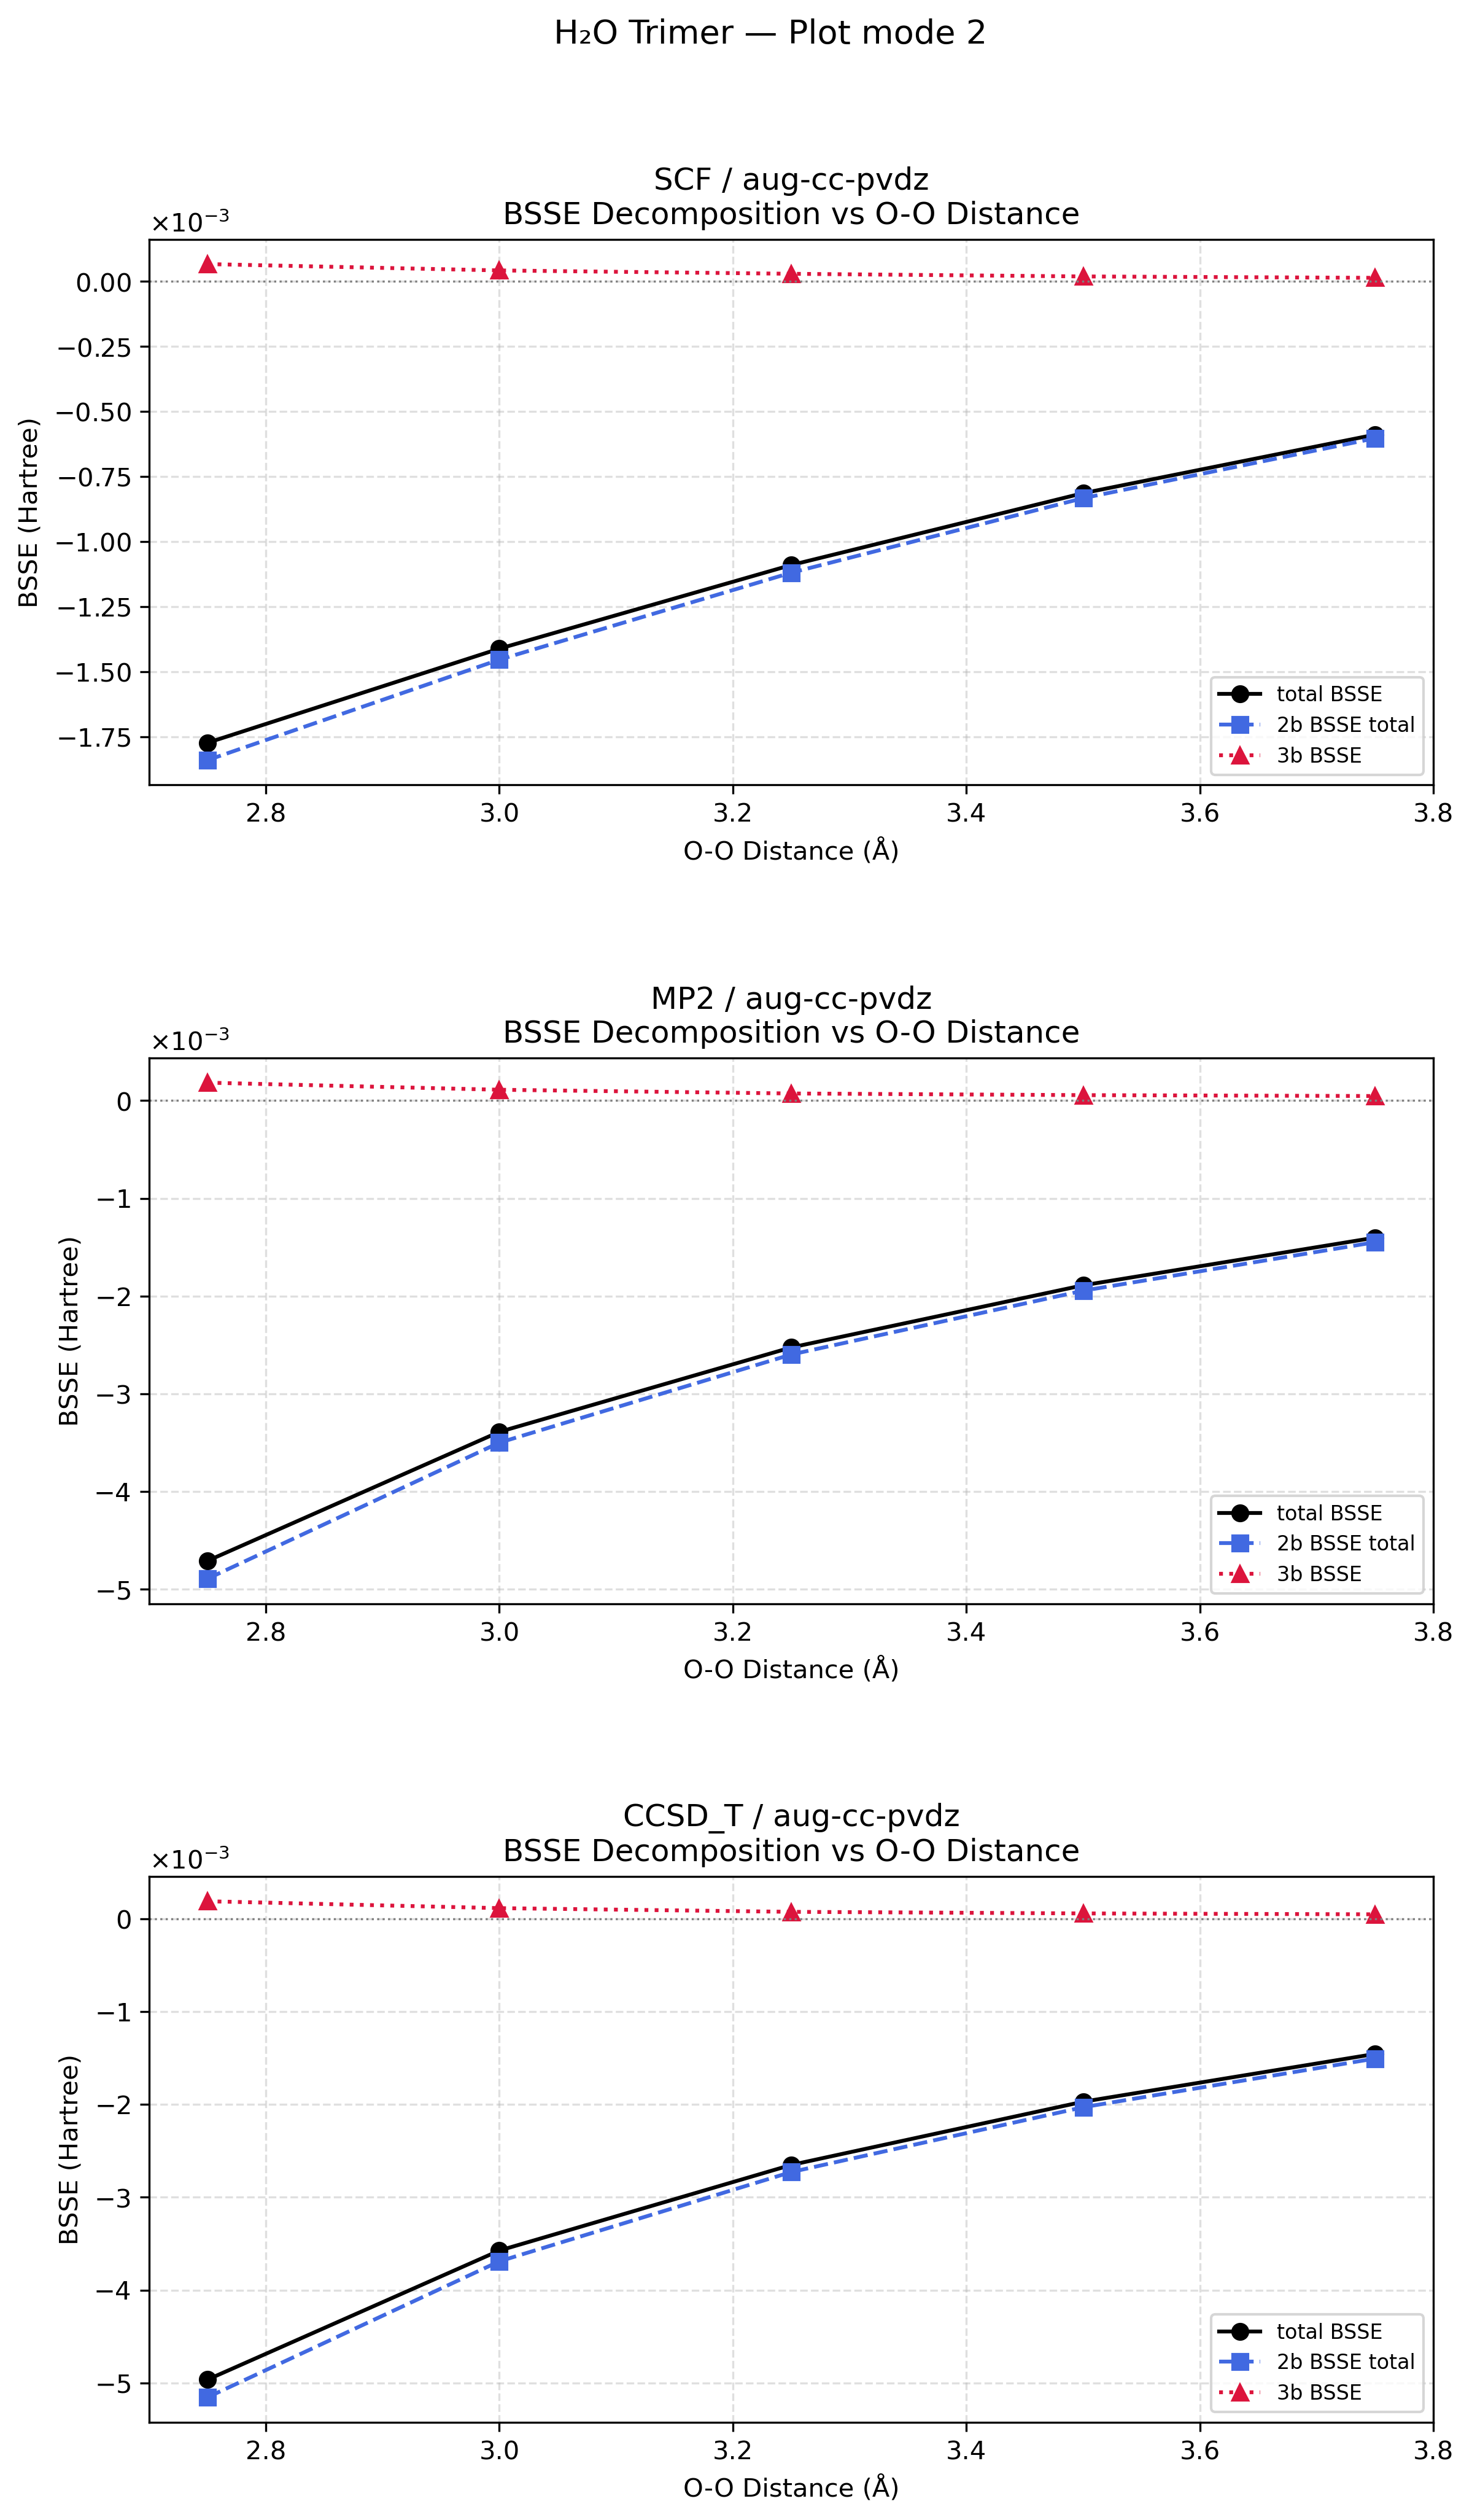
\includegraphics[width=0.7\textwidth]{figures/trimer/H2O_trimer/plot2_all_aug-cc-pvdz.png}
    \caption{BSSE body-order decomposition vs O--O distance $R$ for the
    \ce{H2O} trimer at the aug-cc-pVDZ level. Each panel corresponds to
    one level of theory (SCF, MP2, CCSD(T)). Black circles: total BSSE;
    blue dashed: 2-body total ($\theta^{(2)}$); red triangles: 3-body
    term ($\theta^{(3)}$). The total and 2-body curves are nearly
    indistinguishable in all three panels. The 3-body term is positive
    and remains close to zero across the full range of $R$.}
    \label{fig:h2o_trimer_plot2}
\end{figure}

In all three panels the total BSSE and the 2-body total are nearly
indistinguishable, indicating that the 2-body term accounts for
essentially all of the BSSE. The 3-body contribution $\theta^{(3)}$
is positive in sign (opposite to the 2-body term) and remains close
to zero across the full range of $R$ and all three methods. The
dominance of the 2-body term is consistent across SCF, MP2, and
CCSD(T).

% ----------------------------------------------------------------------
\subsection{Per-Pair Two-Body BSSE}
% ----------------------------------------------------------------------

Figure~\ref{fig:h2o_trimer_plot3} resolves the 2-body BSSE into
contributions from each of the three monomer pairs: AB, AC, and BC.

\begin{figure}[!ht]
    \centering
    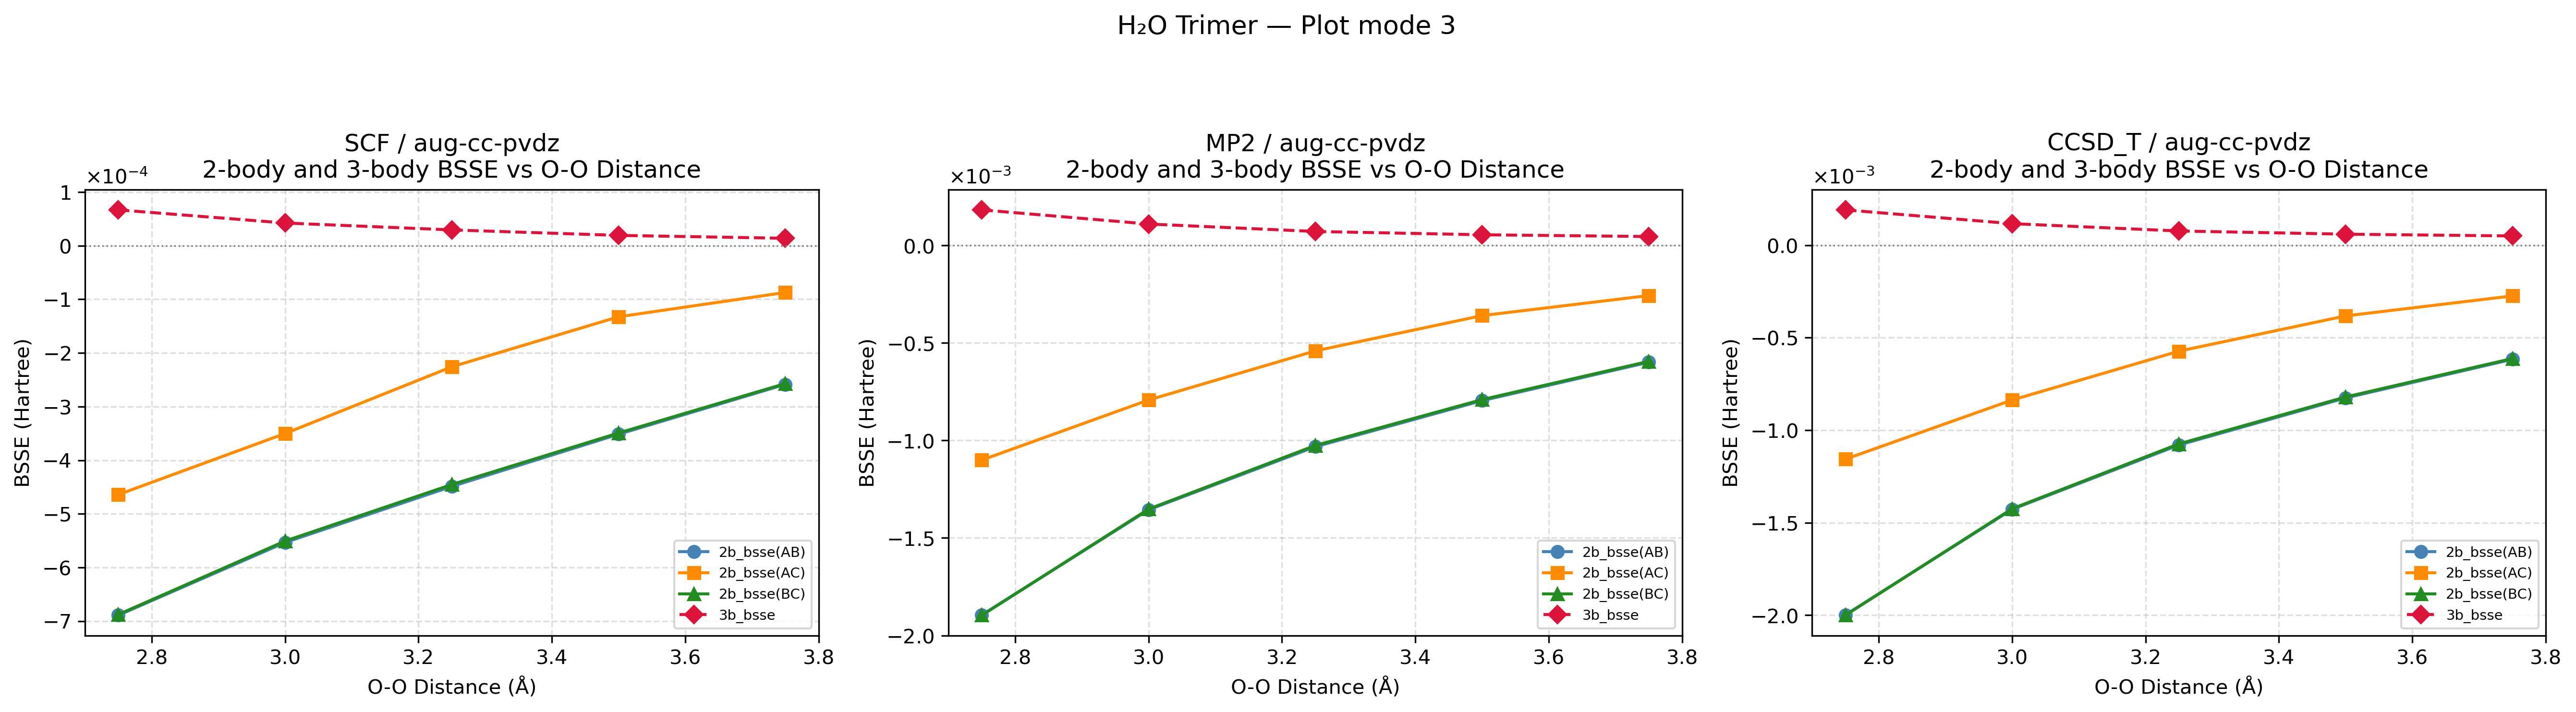
\includegraphics[width=0.7\textwidth]{figures/trimer/H2O_trimer/plot3_all_aug-cc-pvdz.png}
    \caption{Per-pair 2-body and 3-body BSSE vs O--O distance $R$ for
    the \ce{H2O} trimer at the aug-cc-pVDZ level. Each panel
    corresponds to one level of theory. Note the difference in $y$-axis
    scale between the SCF panel ($\times 10^{-4}$~Ha) and the MP2 and
    CCSD(T) panels ($\times 10^{-3}$~Ha). Blue circles: $\theta^{(2)}$(AB);
    orange squares: $\theta^{(2)}$(AC); green triangles: $\theta^{(2)}$(BC);
    red dashed diamonds: $\theta^{(3)}$. The AB and BC pair contributions
    are nearly equal across all methods and distances. The AC pair
    contribution is consistently smaller in magnitude than AB and BC.}
    \label{fig:h2o_trimer_plot3}
\end{figure}

The AB and BC pair contributions are nearly equal at all $R$ values
and across all three methods, while the AC pair contribution is
consistently smaller in magnitude --- approximately half the value of
AB and BC at $R = \SI{3.25}{\angstrom}$ (CCSD(T)). The 3-body term
$\theta^{(3)}$ is positive and small relative to all three pair
contributions.

% TODO: pending PI discussion — physical interpretation of AC pair asymmetry.
% The AC pair has a different relative orientation compared to AB and BC
% in the equilateral triangle geometry (O-O facing geometry), which may
% explain the consistently smaller 2b_bsse(AC). Whether this is due to
% the specific monomer orientation or a more general geometric effect
% requires PI confirmation before asserting in the text.

\clearpage

% ----------------------------------------------------------------------
\subsection{Two-Body BSSE Decomposition at $R = \SI{3.25}{\angstrom}$}
% ----------------------------------------------------------------------

Figure~\ref{fig:h2o_trimer_plot4} shows the FORM~II decomposition of
the 2-body BSSE at the representative configuration $R =
\SI{3.25}{\angstrom}$ (configuration~2) at the CCSD(T) level. Each
pair contribution $\theta^{(2)}(IJ)$ is broken down into its two
monomer-in-dimer-basis $\delta$ terms.

\begin{figure}[!ht]
    \centering
    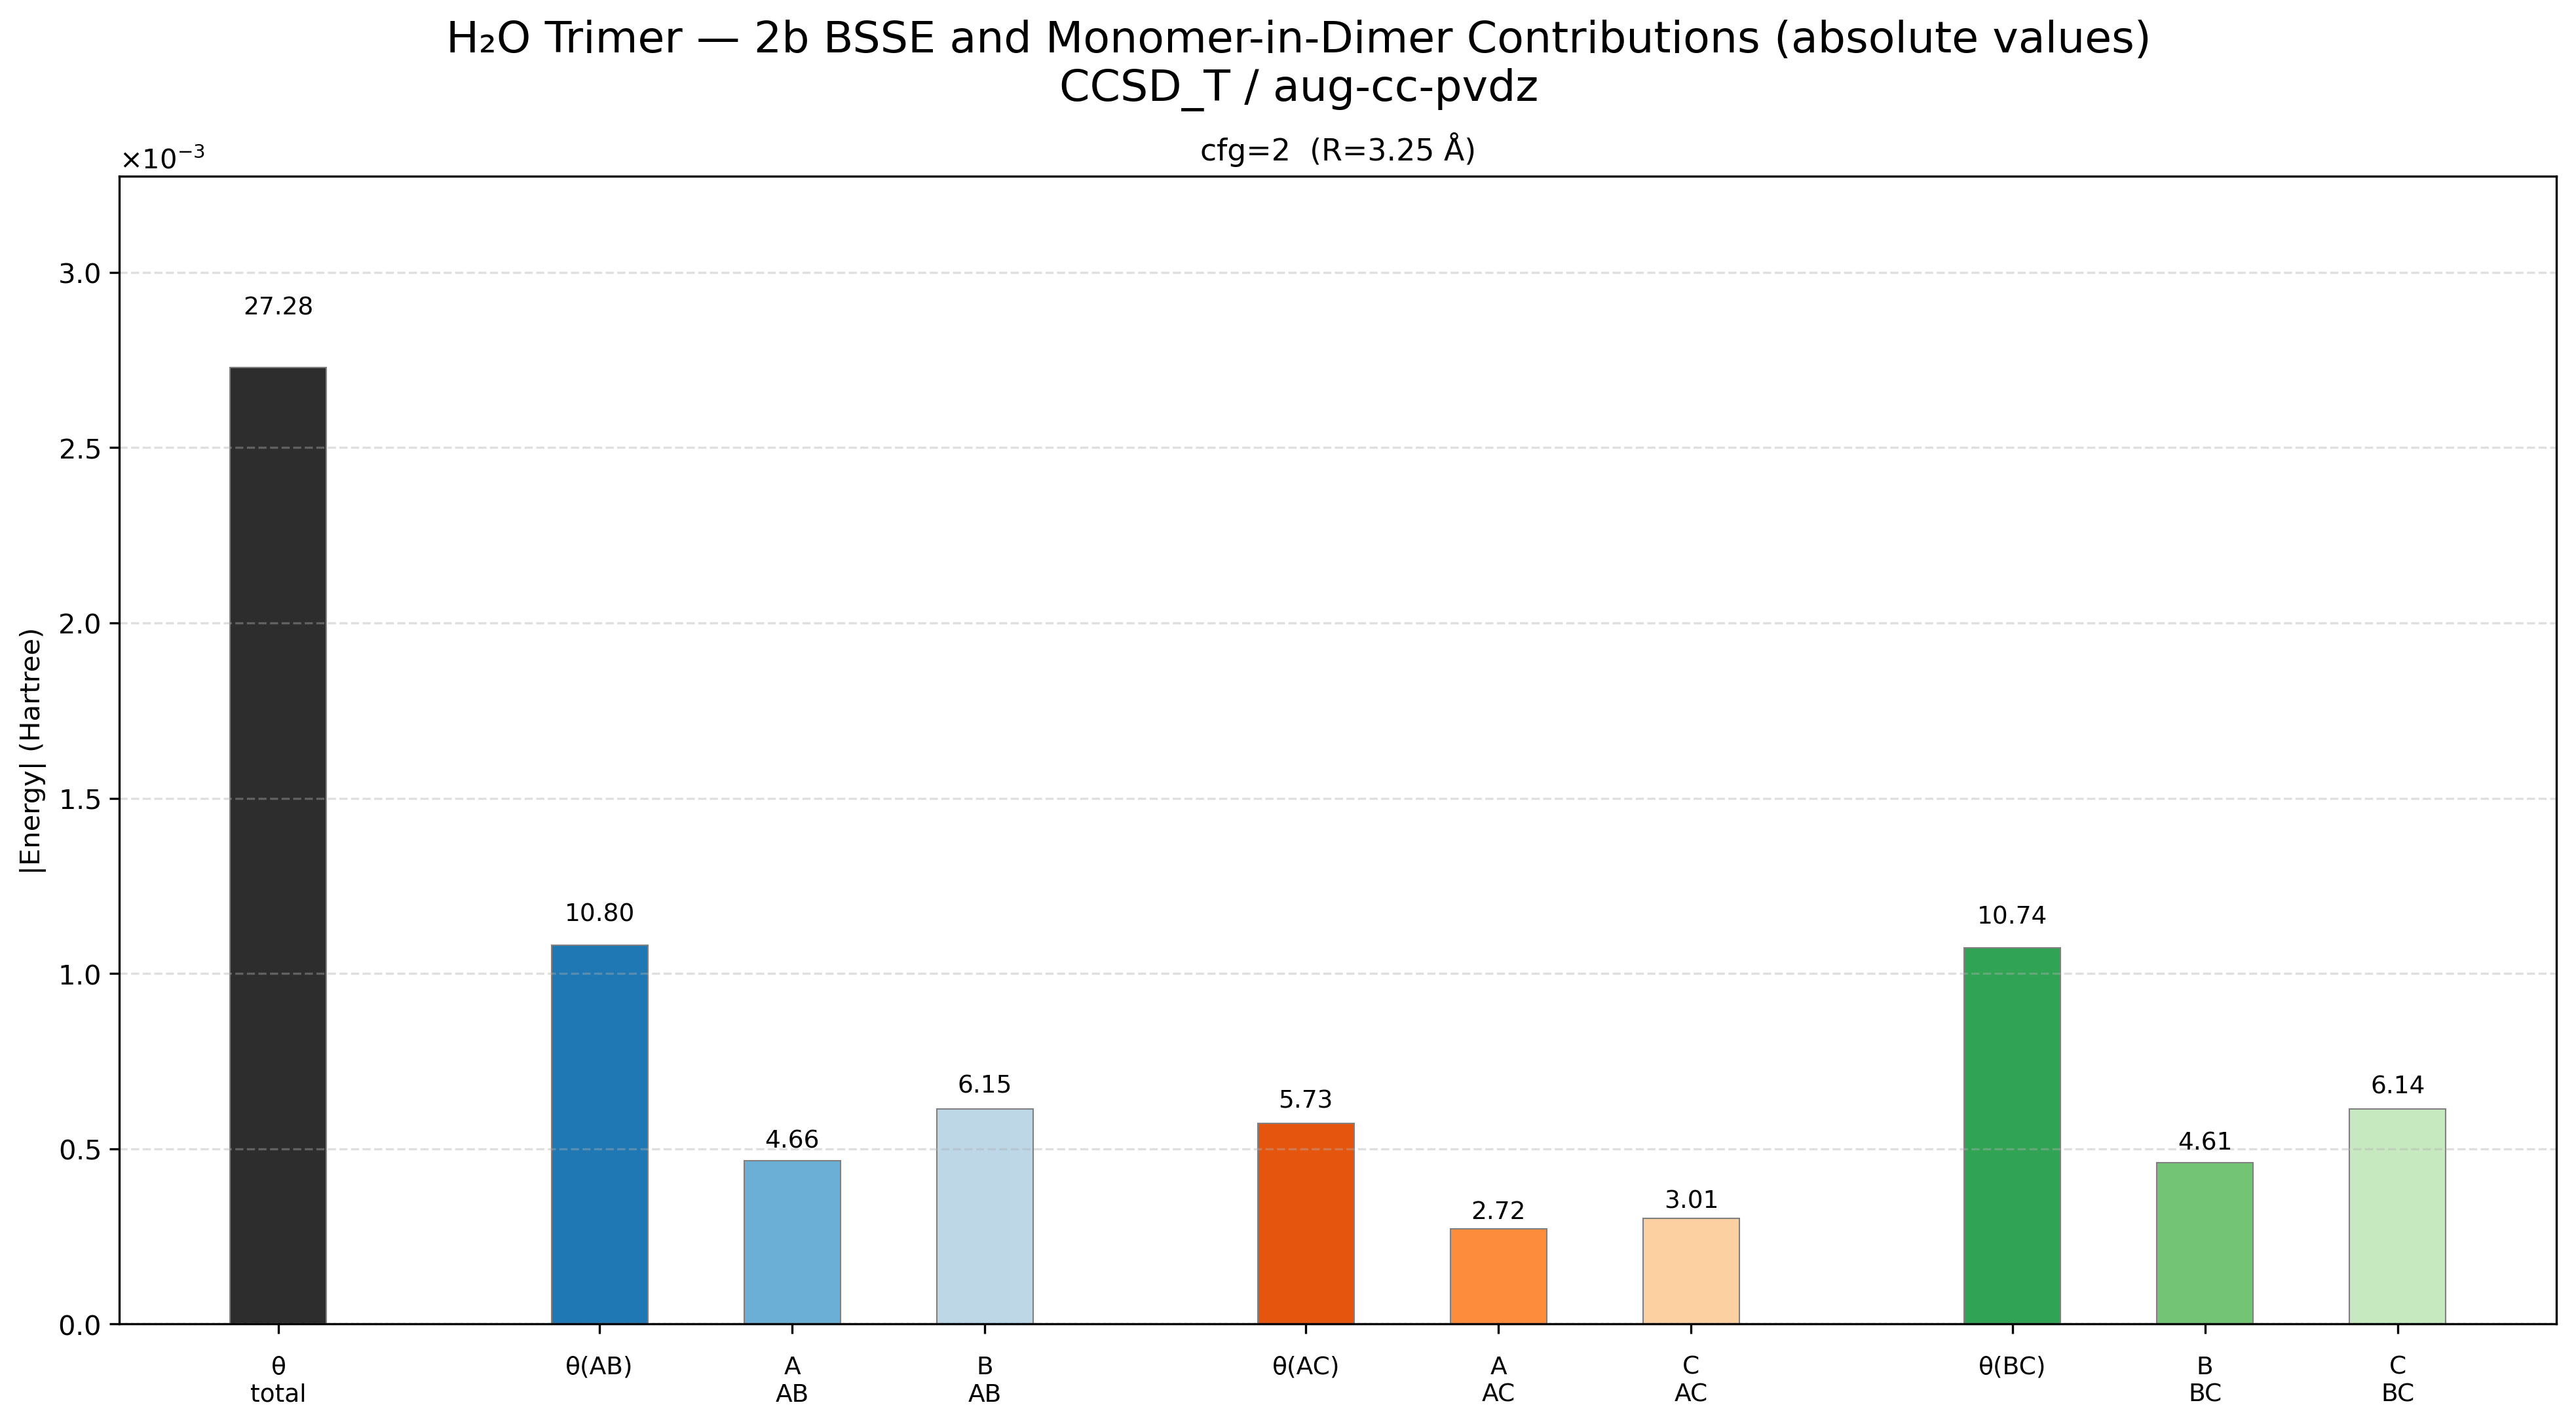
\includegraphics[width=1.0\textwidth]{figures/trimer/H2O_trimer/plot4_CCSD_T_aug-cc-pvdz_part3.png}
    \caption{FORM~II decomposition of the 2-body BSSE for the \ce{H2O}
    trimer at $R = \SI{3.25}{\angstrom}$ (configuration~2), CCSD(T)/aug-cc-pVDZ.
    All values are absolute values in units of $10^{-3}$~Ha. Black bar:
    total 2-body BSSE $|\theta^{(2)}|= 27.28 \times 10^{-3}$~Ha. Dark
    blue and light blue bars: monomer-in-dimer-basis contributions for
    the AB pair ($|\delta(\text{A in AB})| = 4.66$,
    $|\delta(\text{B in AB})| = 6.15$). Orange and light orange bars:
    AC pair contributions ($|\delta(\text{A in AC})| = 2.72$,
    $|\delta(\text{C in AC})| = 3.01$). Dark green and light green bars:
    BC pair contributions ($|\delta(\text{B in BC})| = 4.61$,
    $|\delta(\text{C in BC})| = 6.14$). The AB and BC pairs are
    comparable in magnitude; the AC pair contributions are approximately
    half those of AB and BC.}
    \label{fig:h2o_trimer_plot4}
\end{figure}

At $R = \SI{3.25}{\angstrom}$ the pair totals are $|\theta^{(2)}(\text{AB})| =
10.80 \times 10^{-3}$~Ha, $|\theta^{(2)}(\text{BC})| = 10.74 \times
10^{-3}$~Ha, and $|\theta^{(2)}(\text{AC})| = 5.73 \times 10^{-3}$~Ha.
Within each pair the two monomer-in-dimer-basis contributions are of
comparable magnitude. The same pattern --- AB $\approx$ BC $>$ AC ---
holds across all five configurations and all three levels of theory.

% ----------------------------------------------------------------------
\subsection{Three-Body BSSE Decomposition at $R = \SI{3.25}{\angstrom}$}
% ----------------------------------------------------------------------

Figure~\ref{fig:h2o_trimer_plot5} shows the FORM~II decomposition of
the 3-body BSSE at the same representative configuration.

\begin{figure}[!ht]
    \centering
    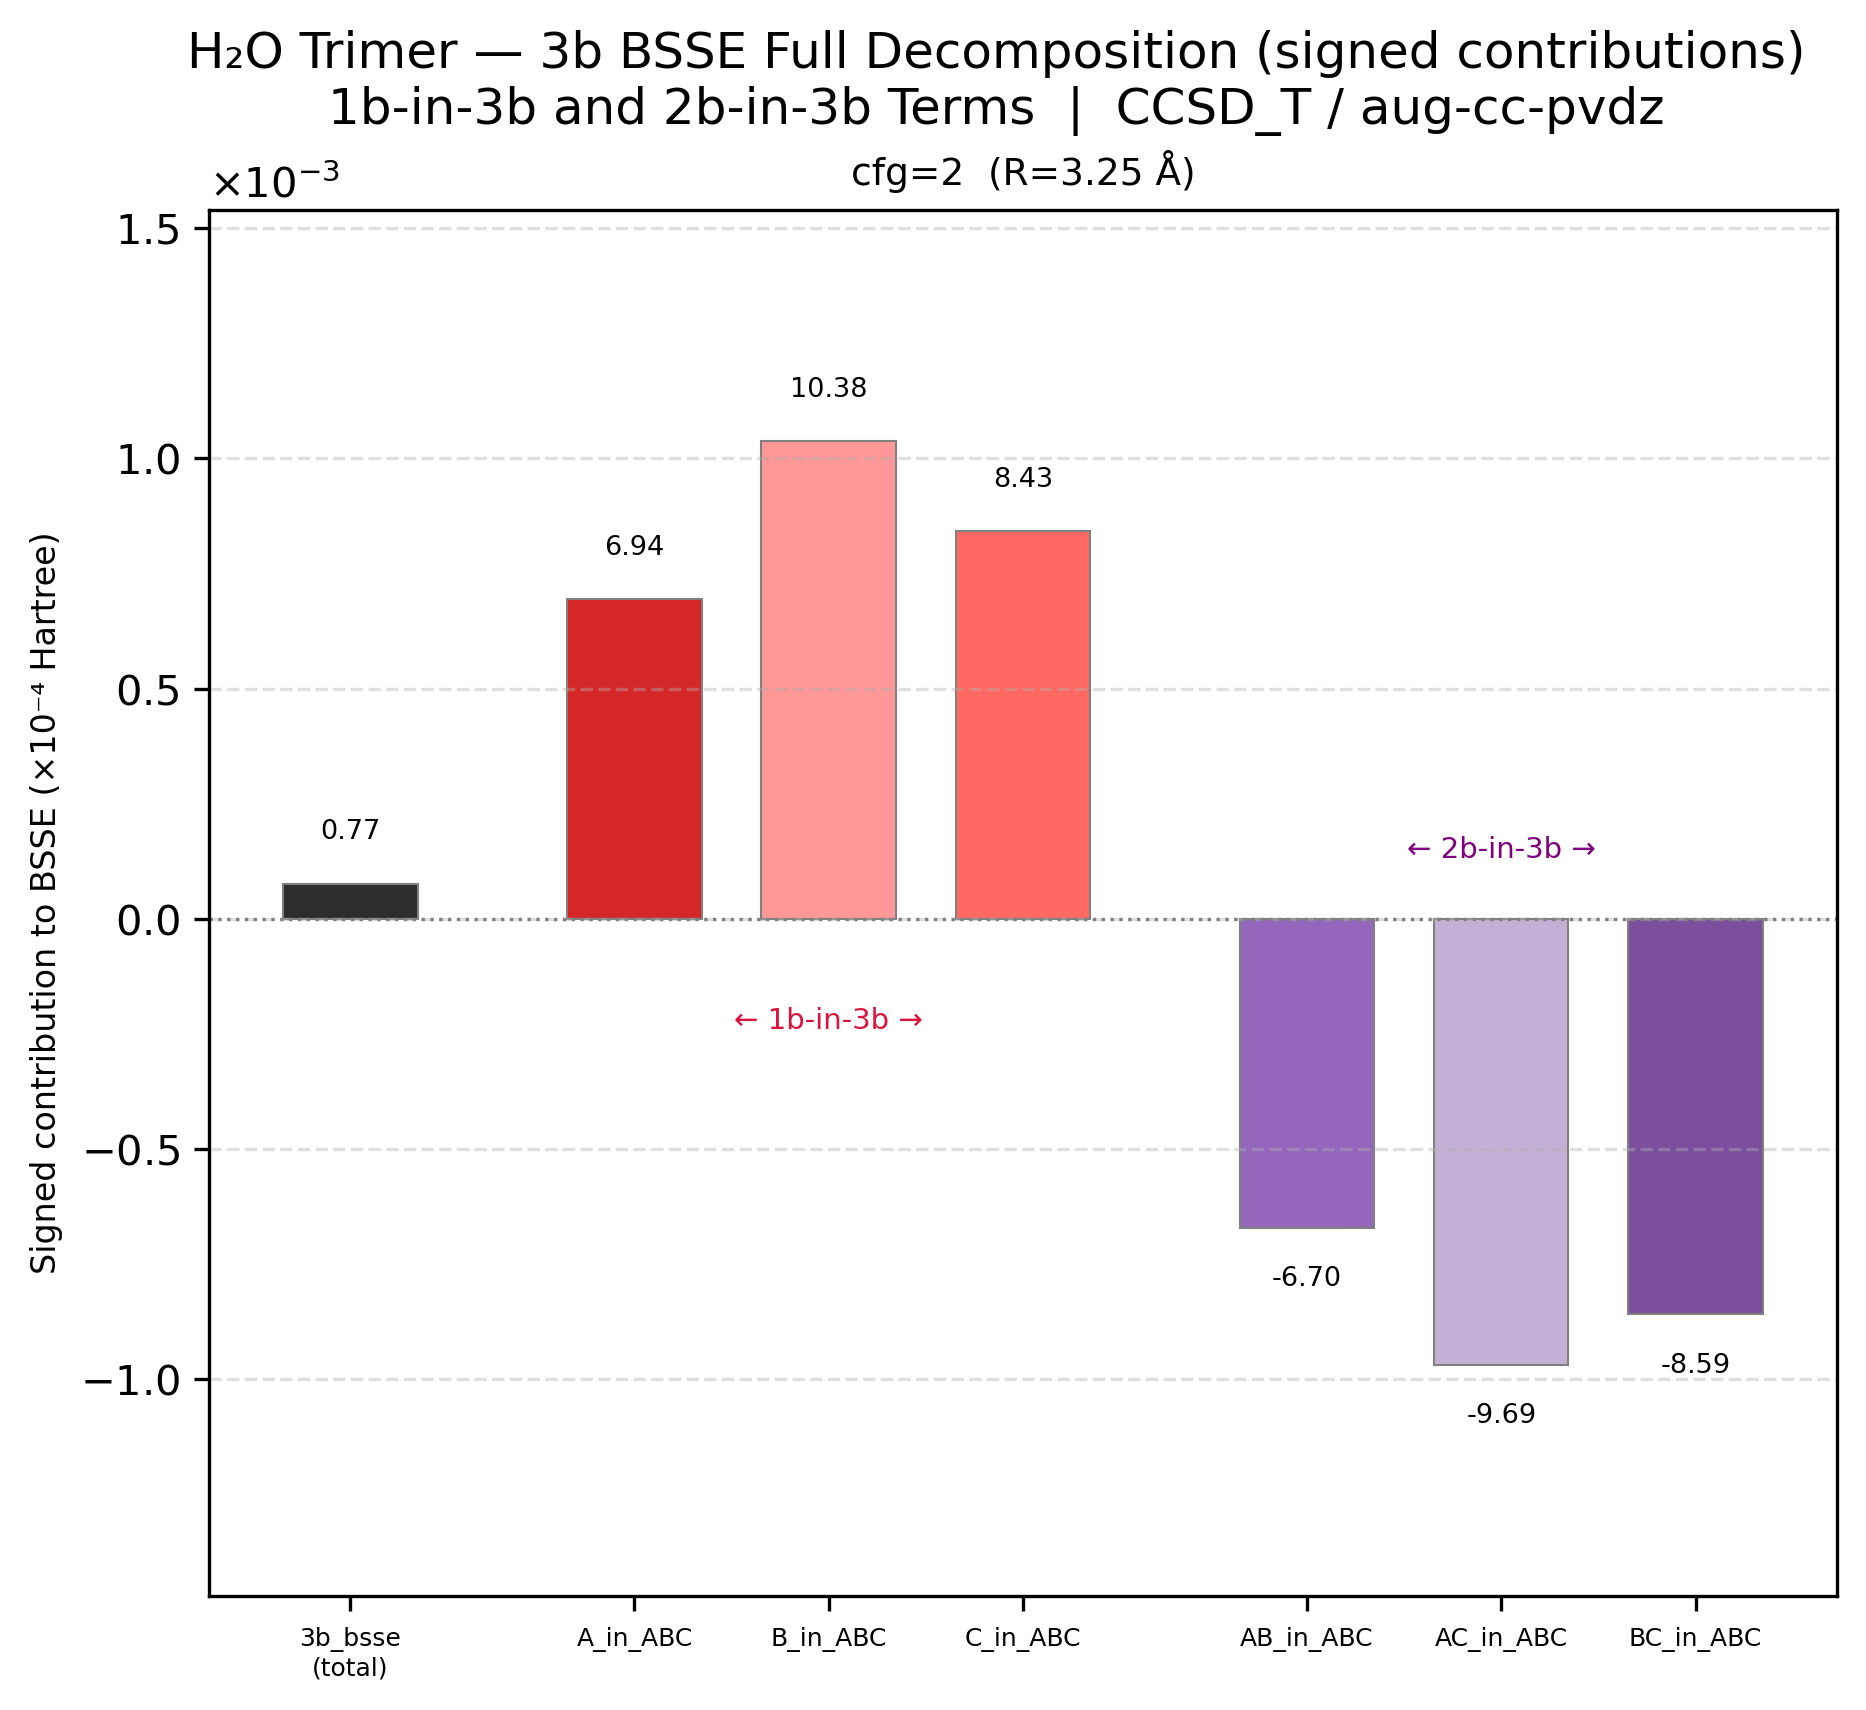
\includegraphics[width=1.0\textwidth]{figures/trimer/H2O_trimer/plot5_CCSD_T_aug-cc-pvdz_part3.png}
    \caption{FORM~II decomposition of the 3-body BSSE for the \ce{H2O}
    trimer at $R = \SI{3.25}{\angstrom}$ (configuration~2),
    CCSD(T)/aug-cc-pVDZ. Signed contributions in units of $10^{-4}$~Ha.
    Black bar: total $\theta^{(3)} = +0.77 \times 10^{-4}$~Ha. Red bars
    (positive): 1b-in-3b terms
    $\delta(\text{A in ABC}) = +6.94$,
    $\delta(\text{B in ABC}) = +10.38$,
    $\delta(\text{C in ABC}) = +8.43$.
    Purple bars (negative): 2b-in-3b terms
    $\delta(\text{AB in ABC}) = -6.70$,
    $\delta(\text{AC in ABC}) = -9.69$,
    $\delta(\text{BC in ABC}) = -8.59$.
    The two groups are opposite in sign and nearly equal in magnitude,
    resulting in a small positive net $\theta^{(3)}$.}
    \label{fig:h2o_trimer_plot5}
\end{figure}

\clearpage

The 3-body BSSE $\theta^{(3)}$ is the result of a near-cancellation
between two groups of opposite sign: the 1b-in-3b terms (positive)
and the 2b-in-3b terms (negative). At $R = \SI{3.25}{\angstrom}$ the
net value is $+0.77 \times 10^{-4}$~Ha, approximately one order of
magnitude smaller than the total 2-body BSSE. This near-cancellation
pattern is consistent across all five configurations.

% ----------------------------------------------------------------------
\subsection{Key Findings}
% ----------------------------------------------------------------------

\begin{finding_box}
\textbf{The 2-body term dominates the \ce{H2O} trimer BSSE.}
Across all five O--O distances and all three levels of theory, the
total BSSE is accounted for almost entirely by the sum of the three
pairwise 2-body contributions. The 3-body term $\theta^{(3)}$ is
positive in sign and approximately one order of magnitude smaller than
the 2-body total at all configurations sampled.
\end{finding_box}

\begin{finding_box}
\textbf{The AC pair contributes less 2-body BSSE than AB or BC.}
The per-pair decomposition shows that $\theta^{(2)}(\text{AB}) \approx
\theta^{(2)}(\text{BC})$ across all configurations and methods, while
$\theta^{(2)}(\text{AC})$ is consistently smaller --- approximately
half the AB and BC values at mid-range distances. The 3-body BSSE
arises from a near-cancellation between the 1b-in-3b (positive) and
2b-in-3b (negative) FORM~II delta terms.
\end{finding_box}

\clearpage

% ======================================================================
\section{Ne Trimer BSSE Results}
% ======================================================================

% ----------------------------------------------------------------------
\subsection{Total BSSE vs Ne--Ne Distance}
% ----------------------------------------------------------------------

Figure~\ref{fig:ne_trimer_plot1} shows the total BSSE as a function of
Ne--Ne distance $R$ for all three levels of theory.

\begin{figure}[!ht]
    \centering
    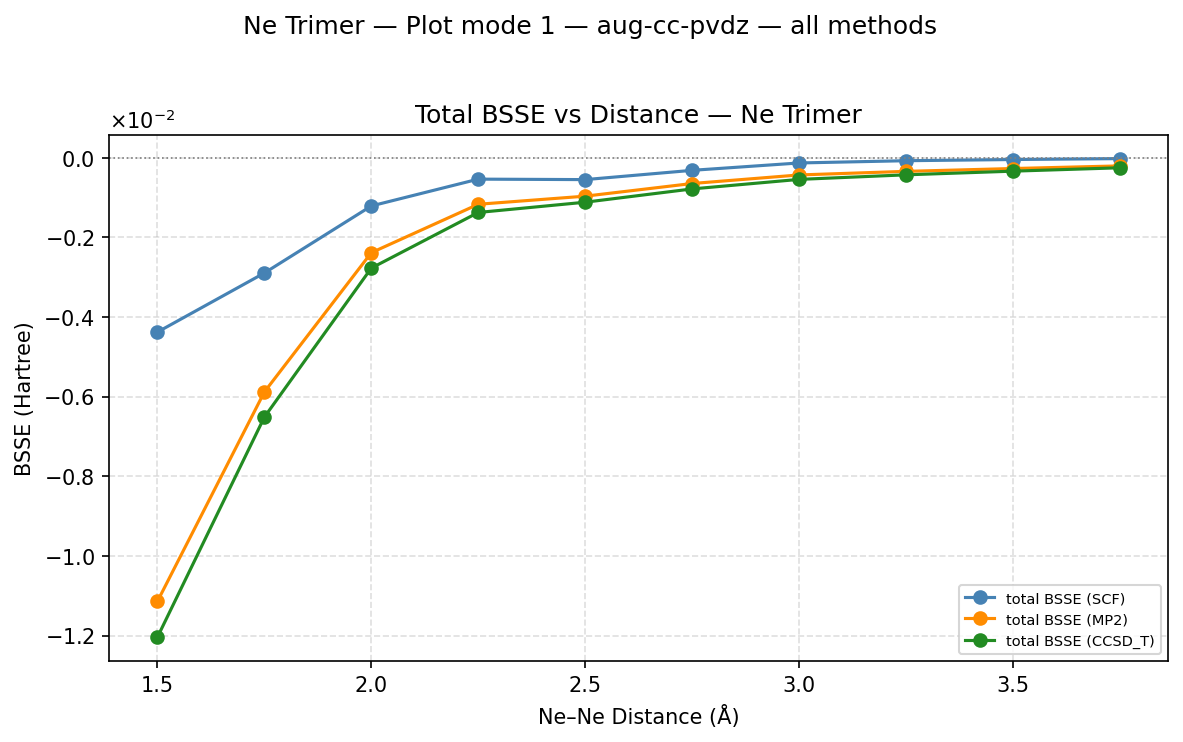
\includegraphics[width=1.0\textwidth]{figures/trimer/Ne_trimer/plot1_Ne_all_aug-cc-pvdz.png}
    \caption{Total BSSE vs Ne--Ne distance $R$ for the Ne trimer at
    the aug-cc-pVDZ level. Blue circles: SCF; orange squares: MP2;
    green triangles: CCSD(T). All values are in Hartree. All three
    curves approach zero monotonically with increasing $R$. At the
    shortest distance ($R = \SI{1.5}{\angstrom}$) the total BSSE
    reaches approximately $-4.5 \times 10^{-3}$~Ha (SCF),
    $-1.1 \times 10^{-2}$~Ha (MP2), and $-1.2 \times 10^{-2}$~Ha
    (CCSD(T)). The MP2 and CCSD(T) curves are close throughout
    the range, while the SCF contribution is smaller in magnitude
    by approximately a factor of three at short range.}
    \label{fig:ne_trimer_plot1}
\end{figure}

All three curves are negative and approach zero monotonically with
increasing $R$, consistent with the reduction of basis set overlap at
larger separations. The BSSE magnitude drops sharply between $R =
\SI{1.5}{\angstrom}$ and $R = \SI{2.0}{\angstrom}$, then decreases
more gradually at longer range. The MP2 and CCSD(T) values are
substantially larger in magnitude than the SCF contribution across the
full range, reflecting the additional basis set incompleteness
introduced by the correlation treatment.

% ----------------------------------------------------------------------
\subsection{Two-Body and Three-Body Decomposition}
% ----------------------------------------------------------------------

Figure~\ref{fig:ne_trimer_plot2} separates the total BSSE into its
two-body ($\theta^{(2)}$) and three-body ($\theta^{(3)}$) components
for each level of theory.

\begin{figure}[!ht]
    \centering
    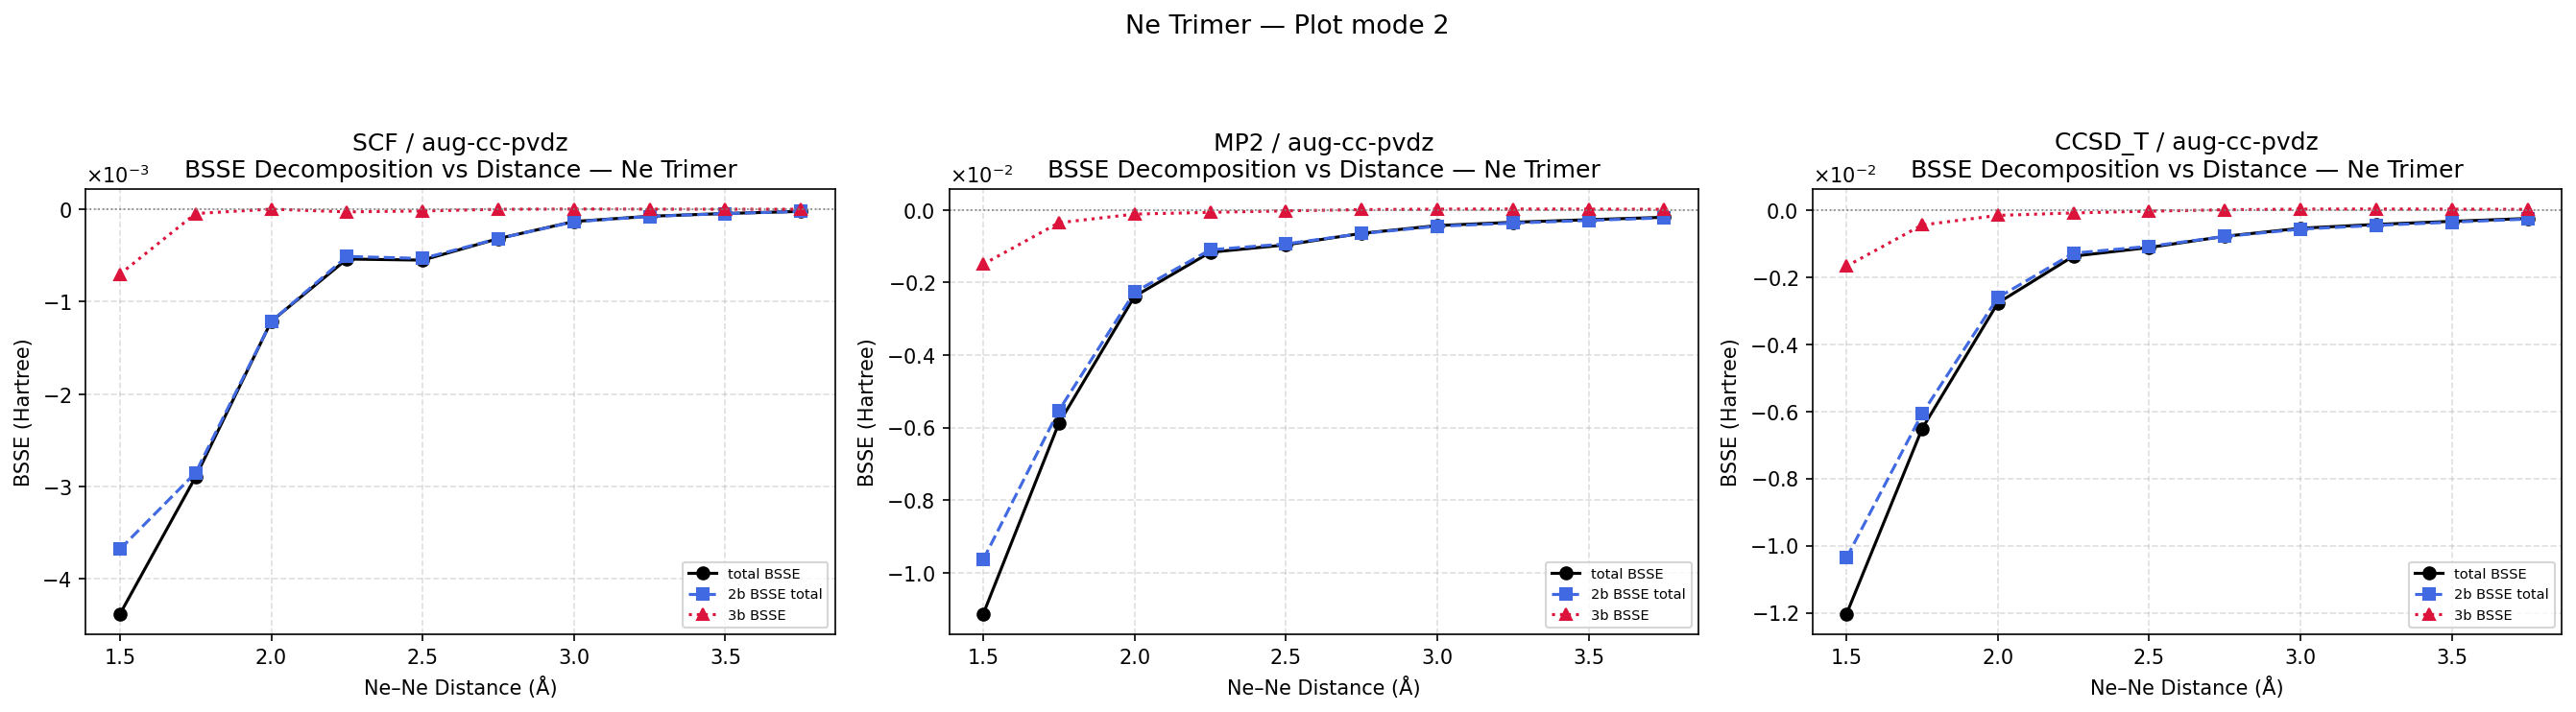
\includegraphics[width=0.7\textwidth]{figures/trimer/Ne_trimer/plot2_Ne_all_aug-cc-pvdz.png}
    \caption{BSSE body-order decomposition vs Ne--Ne distance $R$ for
    the Ne trimer at the aug-cc-pVDZ level. Each panel corresponds to
    one level of theory (SCF, MP2, CCSD(T)). Black circles: total
    BSSE; blue dashed squares: 2-body total ($\theta^{(2)}$); red
    dashed triangles: 3-body term ($\theta^{(3)}$). The total and
    2-body curves are nearly indistinguishable in all three panels.
    At all three levels of theory the 3-body term is negative at short
    range and changes sign to positive with increasing $R$, crossing
    zero near $R = \SI{2.75}{\angstrom}$.}
    \label{fig:ne_trimer_plot2}
\end{figure}

In all three panels the total BSSE and the 2-body total are nearly
indistinguishable, confirming that the 2-body term accounts for
essentially all of the BSSE. The 3-body contribution $\theta^{(3)}$
is small in magnitude relative to the 2-body total at all distances.
A notable feature present at all three levels of theory is a sign
change in $\theta^{(3)}$: the term is negative at short range (where
orbital overlap is significant) and becomes positive at longer range,
crossing zero near $R = \SI{2.75}{\angstrom}$.

% ----------------------------------------------------------------------
\subsection{Per-Pair Two-Body BSSE}
% ----------------------------------------------------------------------

Figure~\ref{fig:ne_trimer_plot3} resolves the 2-body BSSE into
contributions from each of the three monomer pairs: AB, AC, and BC.

\begin{figure}[!ht]
    \centering
    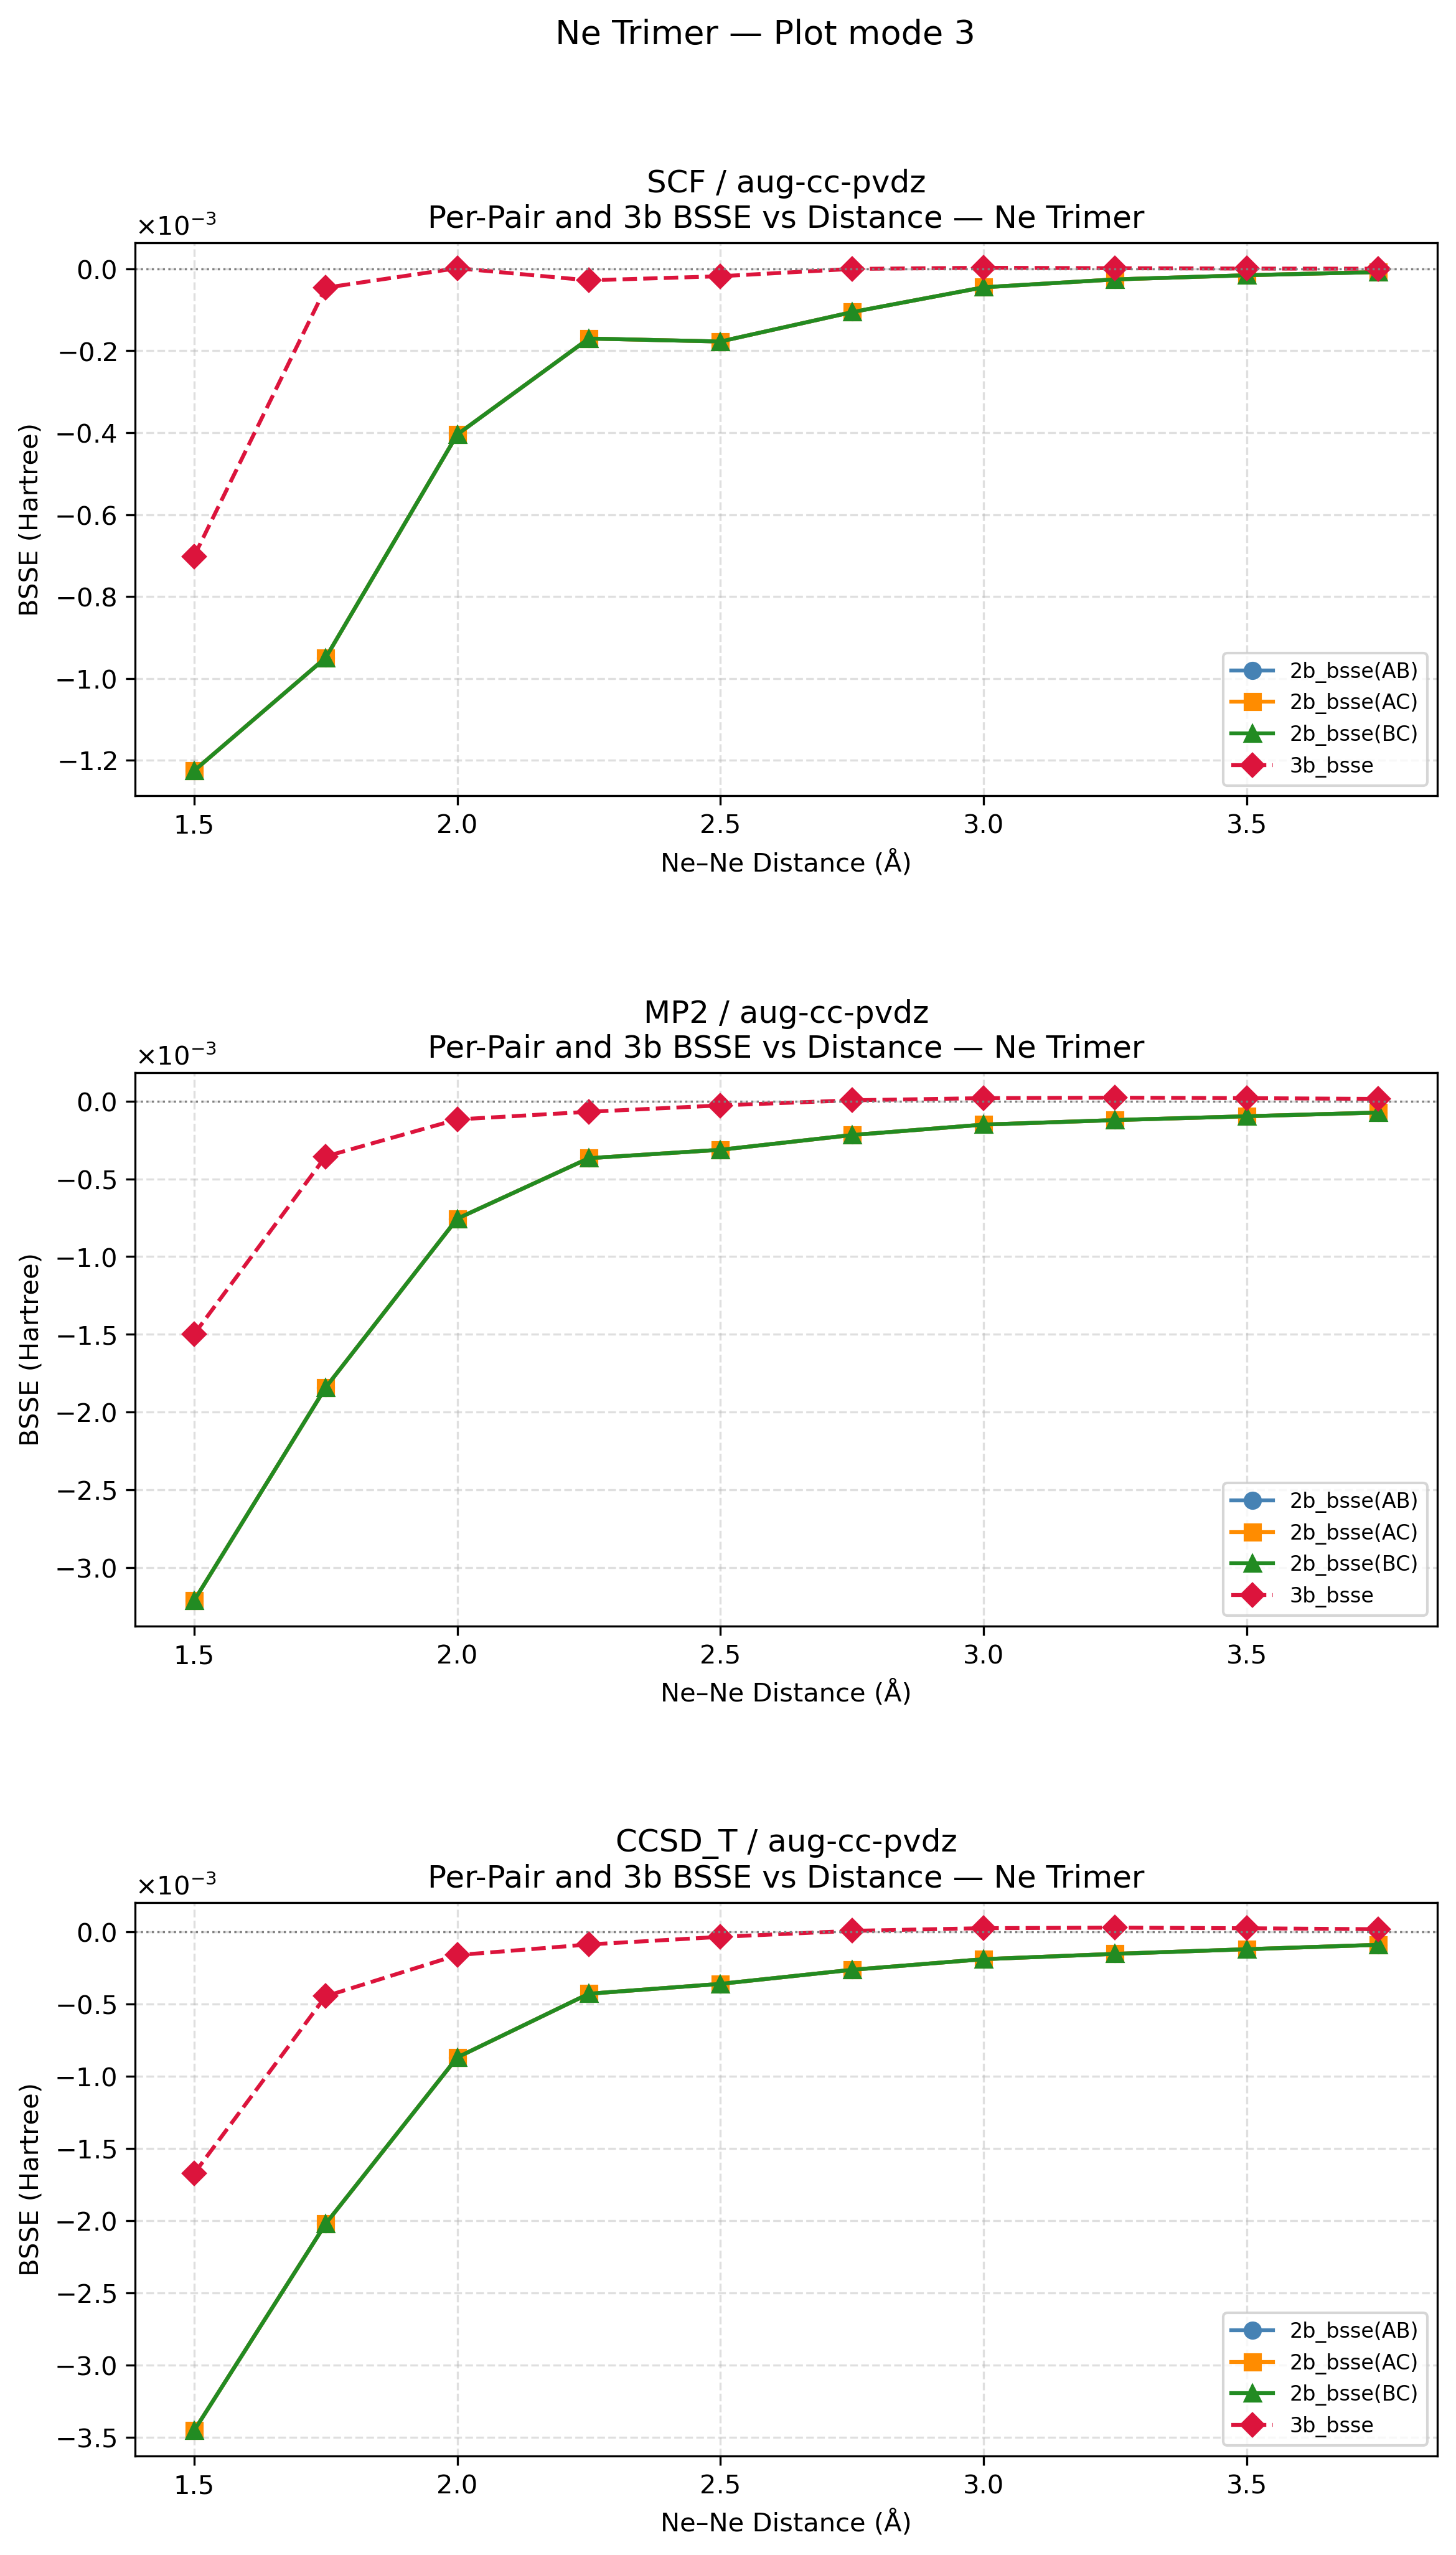
\includegraphics[width=0.7\textwidth]{figures/trimer/Ne_trimer/plot3_Ne_all_aug-cc-pvdz.png}
    \caption{Per-pair 2-body and 3-body BSSE vs Ne--Ne distance $R$
    for the Ne trimer at the aug-cc-pVDZ level. Each panel corresponds
    to one level of theory. Blue circles: $\theta^{(2)}$(AB); orange
    squares: $\theta^{(2)}$(AC); green triangles: $\theta^{(2)}$(BC);
    red dashed diamonds: $\theta^{(3)}$. The three pair contributions
    are exactly equal at every distance and every level of theory,
    reflecting the perfect equilateral symmetry of the Ne trimer:
    $\theta^{(2)}(\text{AB}) = \theta^{(2)}(\text{AC}) =
    \theta^{(2)}(\text{BC})$ at all $R$.}
    \label{fig:ne_trimer_plot3}
\end{figure}

The three pair contributions $\theta^{(2)}(\text{AB})$,
$\theta^{(2)}(\text{AC})$, and $\theta^{(2)}(\text{BC})$ are
numerically identical at every configuration and every level of
theory. In Figure~\ref{fig:ne_trimer_plot3} the three symbols lie
exactly on top of one another, reducing to a single visible curve.
This perfect degeneracy is a direct consequence of the equilateral
triangle geometry and the identity of the Ne monomers: all three
pairs are related by the $C_{3v}$ symmetry of the cluster. In
contrast to the \ce{H2O} trimer, where the AC pair showed a
consistently distinct BSSE from AB and BC, the Ne trimer exhibits
no such pair inequivalence.

\clearpage

% ----------------------------------------------------------------------
\subsection{Two-Body BSSE Decomposition at $R = \SI{2.5}{\angstrom}$}
% ----------------------------------------------------------------------

Figure~\ref{fig:ne_trimer_plot4} shows the FORM~II decomposition of
the 2-body BSSE at the representative configuration $R =
\SI{2.5}{\angstrom}$ (configuration~4) at the CCSD(T) level. Each
pair contribution $\theta^{(2)}(IJ)$ is broken down into its two
monomer-in-dimer-basis $\delta$ terms.

\begin{figure}[!ht]
    \centering
    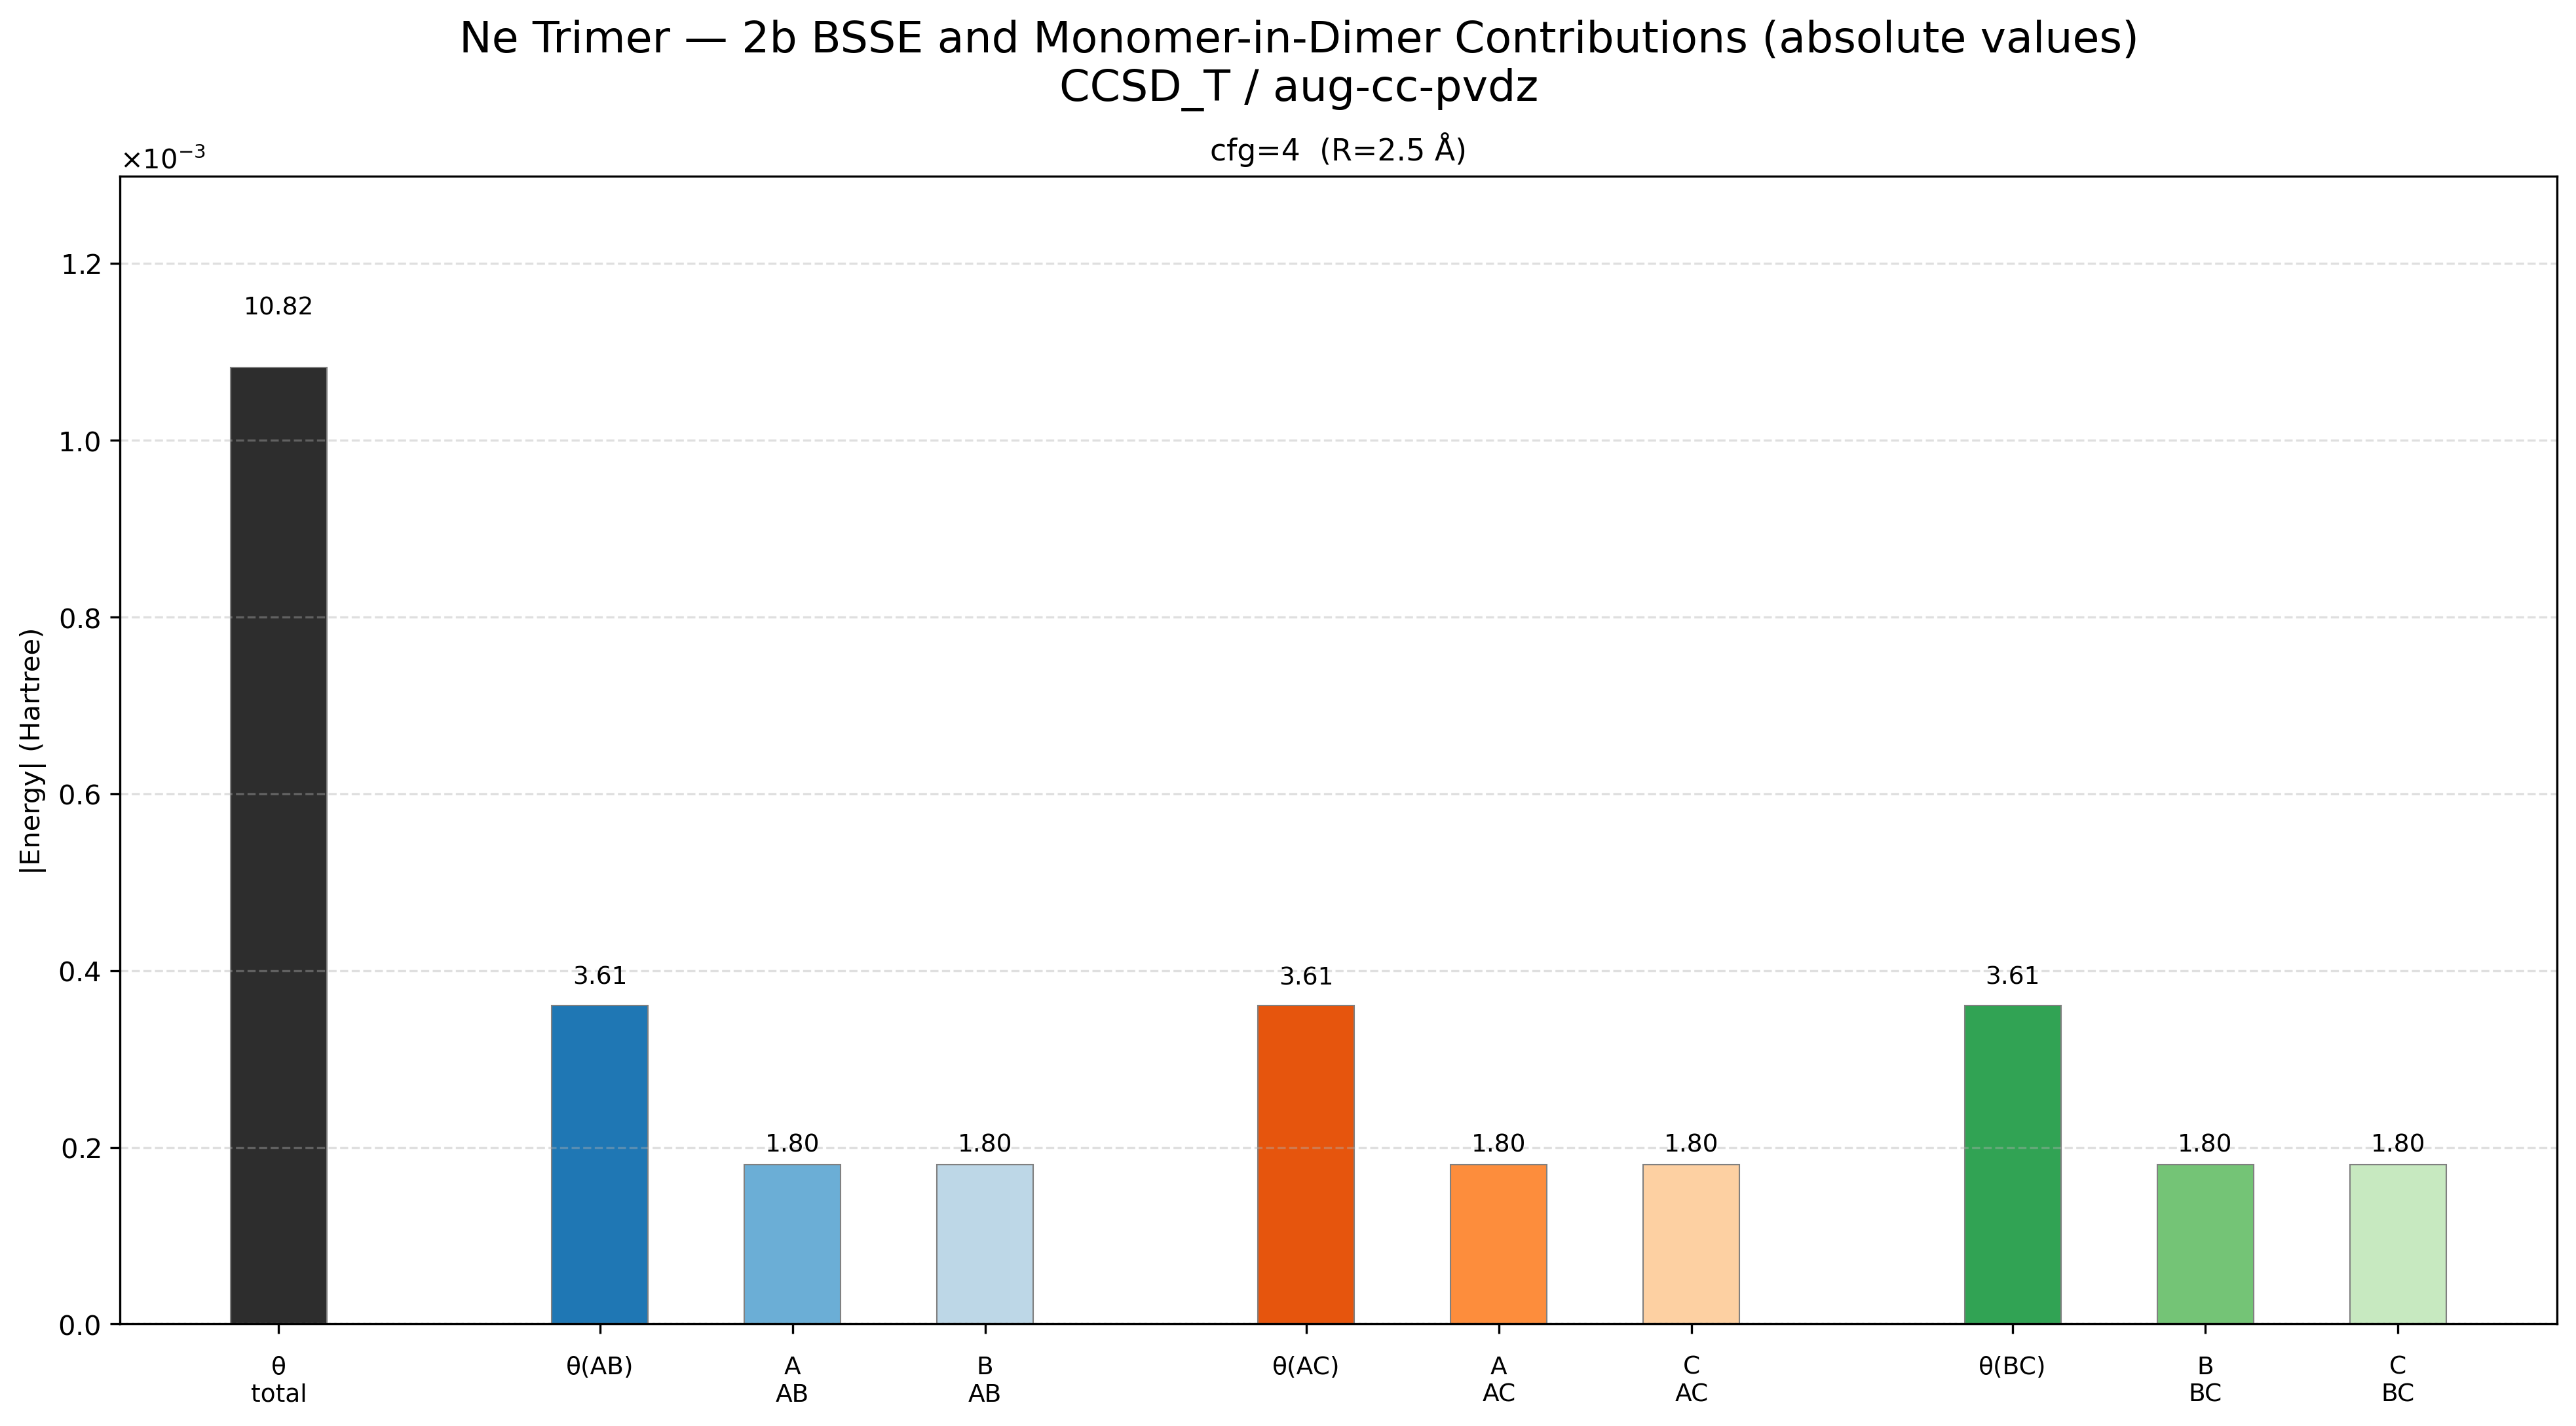
\includegraphics[width=1.0\textwidth]{figures/trimer/Ne_trimer/plot4_Ne_CCSD_T_aug-cc-pvdz_part5.png}
    \caption{FORM~II decomposition of the 2-body BSSE for the Ne
    trimer at $R = \SI{2.5}{\angstrom}$ (configuration~4),
    CCSD(T)/aug-cc-pVDZ. All values are absolute values in units
    of $10^{-3}$~Ha. Black bar: total 2-body BSSE
    $|\theta^{(2)}| = 10.82 \times 10^{-3}$~Ha. For each pair
    (AB, AC, BC) the pair total is $3.61 \times 10^{-3}$~Ha,
    and the two monomer-in-dimer-basis contributions are each
    $1.80 \times 10^{-3}$~Ha. All nine per-pair and
    per-monomer bars are identical, reflecting the perfect $C_{3v}$
    symmetry of the Ne trimer.}
    \label{fig:ne_trimer_plot4}
\end{figure}

At $R = \SI{2.5}{\angstrom}$ all three pair totals are equal:
$|\theta^{(2)}(\text{AB})| = |\theta^{(2)}(\text{AC})| =
|\theta^{(2)}(\text{BC})| = 3.61 \times 10^{-3}$~Ha. Within each
pair, the two monomer-in-dimer-basis contributions are also equal
($1.80 \times 10^{-3}$~Ha each), as required by the symmetry of the
equilateral triangle. The total 2-body BSSE is simply three times the
per-pair value: $3 \times 3.61 = 10.82 \times 10^{-3}$~Ha. This
complete equivalence of all bars in the decomposition is qualitatively
different from the \ce{H2O} trimer, where the AC pair was consistently
smaller than AB and BC.

% ----------------------------------------------------------------------
\subsection{Three-Body BSSE Decomposition at $R = \SI{2.5}{\angstrom}$}
% ----------------------------------------------------------------------

Figure~\ref{fig:ne_trimer_plot5} shows the FORM~II decomposition of
the 3-body BSSE at the same representative configuration.

\begin{figure}[!ht]
    \centering
    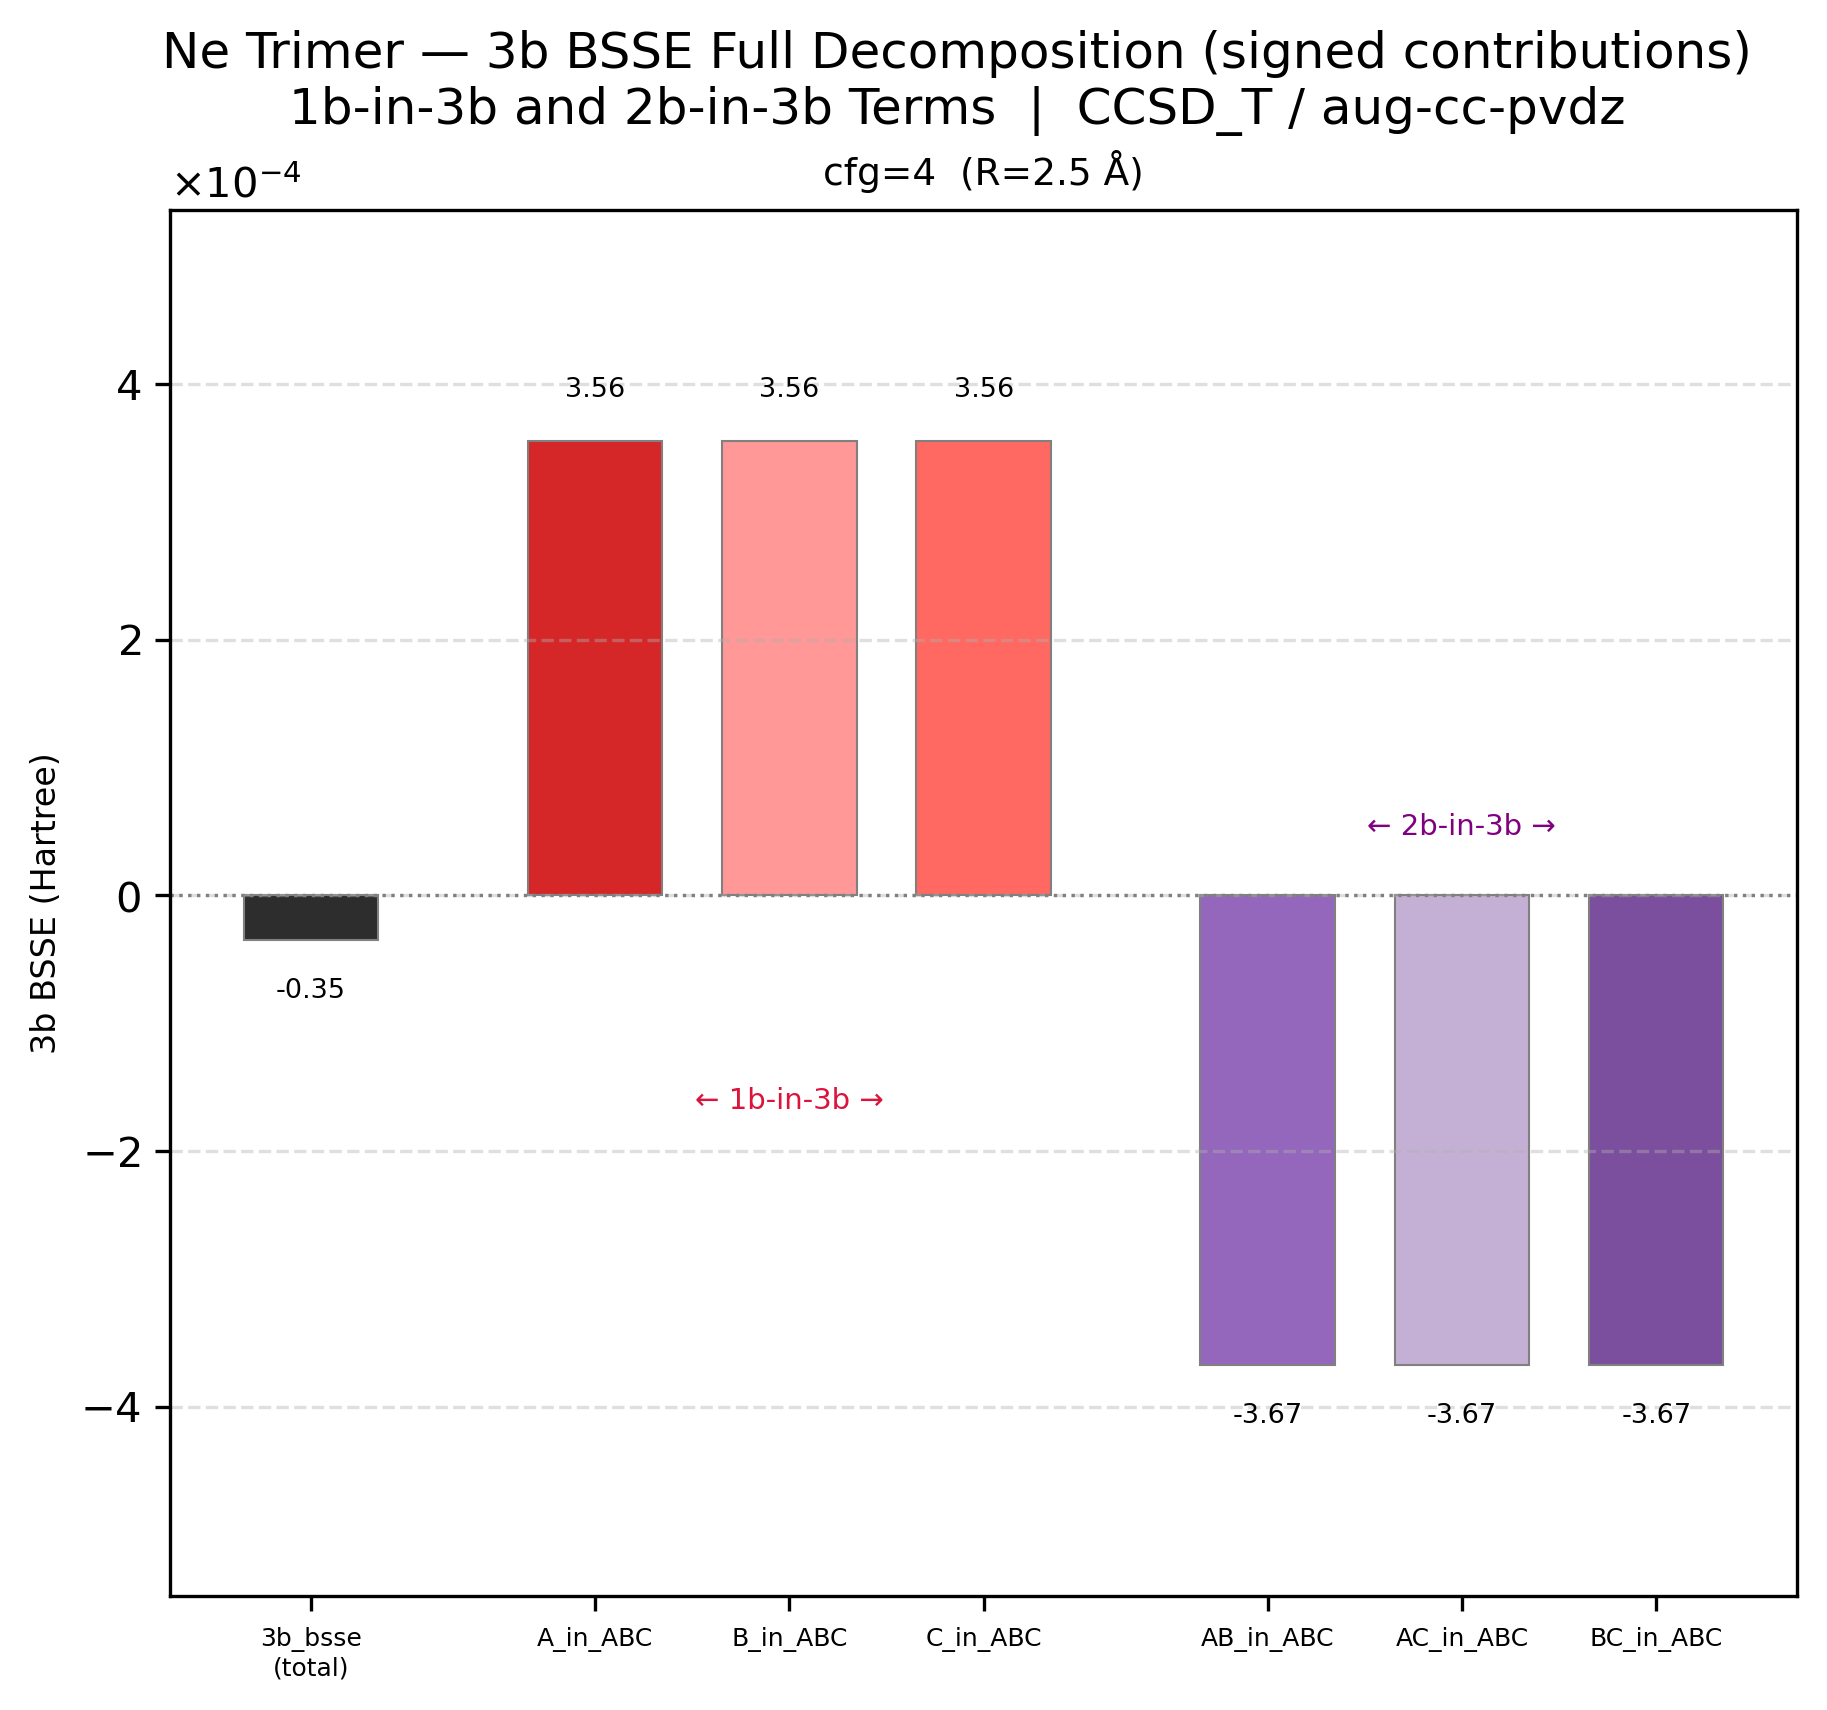
\includegraphics[width=1.0\textwidth]{figures/trimer/Ne_trimer/plot5_Ne_CCSD_T_aug-cc-pvdz_part5.png}
    \caption{FORM~II decomposition of the 3-body BSSE for the Ne
    trimer at $R = \SI{2.5}{\angstrom}$ (configuration~4),
    CCSD(T)/aug-cc-pVDZ. Signed contributions in units of
    $10^{-4}$~Ha. Black bar: total $\theta^{(3)} = -0.35 \times
    10^{-4}$~Ha. Red bars (positive): 1b-in-3b terms
    $\delta(\text{A in ABC}) = \delta(\text{B in ABC}) =
    \delta(\text{C in ABC}) = +3.56 \times 10^{-4}$~Ha.
    Purple bars (negative): 2b-in-3b terms
    $\delta(\text{AB in ABC}) = \delta(\text{AC in ABC}) =
    \delta(\text{BC in ABC}) = -3.67 \times 10^{-4}$~Ha.
    The two groups nearly cancel; the 2b-in-3b terms are slightly
    larger in magnitude, yielding a small negative net
    $\theta^{(3)}$ at this configuration.}
    \label{fig:ne_trimer_plot5}
\end{figure}

\clearpage

The 3-body BSSE $\theta^{(3)}$ again results from a near-cancellation
between the 1b-in-3b terms (positive, $+3.56 \times 10^{-4}$~Ha each)
and the 2b-in-3b terms (negative, $-3.67 \times 10^{-4}$~Ha each).
At $R = \SI{2.5}{\angstrom}$ the 2b-in-3b group is slightly larger
in magnitude, giving a net $\theta^{(3)} = -0.35 \times 10^{-4}$~Ha.
This configuration lies just below the sign-change distance: at $R
\geq \SI{2.75}{\angstrom}$ the 1b-in-3b terms come to dominate and
$\theta^{(3)}$ becomes positive at the MP2 and CCSD(T) levels. As
with the 2-body decomposition, all bars within each group are exactly
equal, a consequence of the perfect $C_{3v}$ symmetry.

% ----------------------------------------------------------------------
\subsection{Key Findings}
% ----------------------------------------------------------------------

\begin{finding_box}
\textbf{Perfect $C_{3v}$ symmetry makes all pair contributions
identical.}
Because the Ne trimer is an equilateral triangle of identical atoms,
$\theta^{(2)}(\text{AB}) = \theta^{(2)}(\text{AC}) =
\theta^{(2)}(\text{BC})$ at every configuration and every level of
theory. All FORM~II delta terms within each body-order group are also
equal. This is in contrast to the \ce{H2O} trimer, where the distinct
monomer orientations break the equivalence of the three pairs.
\end{finding_box}

\begin{finding_box}
\textbf{The 3-body BSSE changes sign with increasing Ne--Ne distance.}
At all three levels of theory the 3-body term $\theta^{(3)}$ is
negative at short range and becomes positive near $R =
\SI{2.75}{\angstrom}$. In all cases the magnitude of $\theta^{(3)}$
remains small relative to the 2-body total, and the 2-body term
dominates the total BSSE across the full range of distances sampled.
\end{finding_box}

\clearpage

% ======================================================================
\section{HF Trimer BSSE Results}
% ======================================================================

% ----------------------------------------------------------------------
\subsection{Total BSSE vs F--F Distance}
% ----------------------------------------------------------------------

Figure~\ref{fig:hf_trimer_plot1} shows the total BSSE as a function of
F--F distance $R$ for all three levels of theory.

\begin{figure}[!ht]
    \centering
    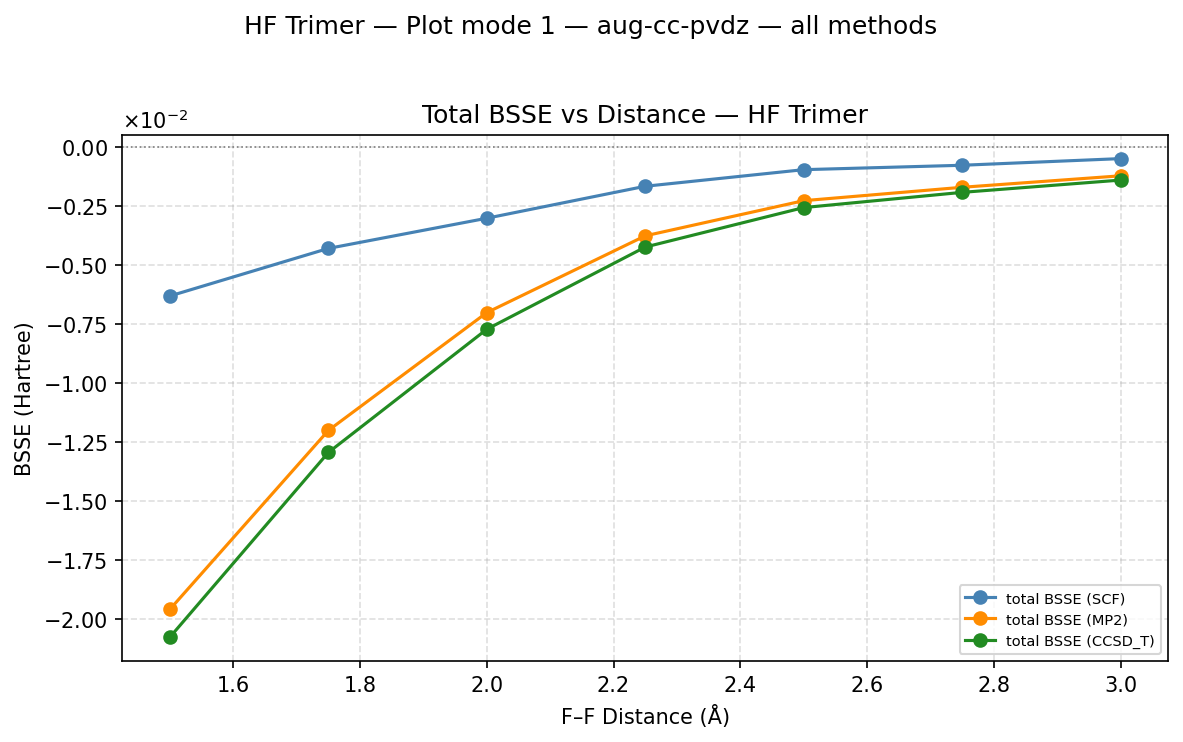
\includegraphics[width=1.0\textwidth]{figures/trimer/HF_trimer/plot1_HF_all_aug-cc-pvdz.png}
    \caption{Total BSSE vs F--F distance $R$ for the HF trimer at
    the aug-cc-pVDZ level. Blue circles: SCF; orange squares: MP2;
    green triangles: CCSD(T). All values are in Hartree. All three
    curves approach zero monotonically with increasing $R$. At the
    shortest distance ($R = \SI{1.5}{\angstrom}$) the total BSSE
    reaches approximately $-6.5 \times 10^{-3}$~Ha (SCF),
    $-1.95 \times 10^{-2}$~Ha (MP2), and $-2.1 \times 10^{-2}$~Ha
    (CCSD(T)). Unlike the Ne and \ce{H2O} trimers, the MP2 and
    CCSD(T) curves are significantly larger in magnitude than the
    SCF contribution across the full range, reflecting the strong
    hydrogen-bonding network in the HF cluster.}
    \label{fig:hf_trimer_plot1}
\end{figure}

All three curves are negative and approach zero monotonically with
increasing $R$. The BSSE magnitude is substantially larger for the
HF trimer than for either the Ne or \ce{H2O} trimers at comparable
distances, consistent with the larger basis sets required to describe
the fluorine lone pairs and the H-bond donor--acceptor interactions.
The MP2 and CCSD(T) values are approximately three times larger in
magnitude than the SCF contribution at short range, a significantly
greater correlated enhancement than observed for the other two
molecules.

% ----------------------------------------------------------------------
\subsection{Two-Body and Three-Body Decomposition}
% ----------------------------------------------------------------------

Figure~\ref{fig:hf_trimer_plot2} separates the total BSSE into its
two-body ($\theta^{(2)}$) and three-body ($\theta^{(3)}$) components
for each level of theory.

\begin{figure}[!ht]
    \centering
    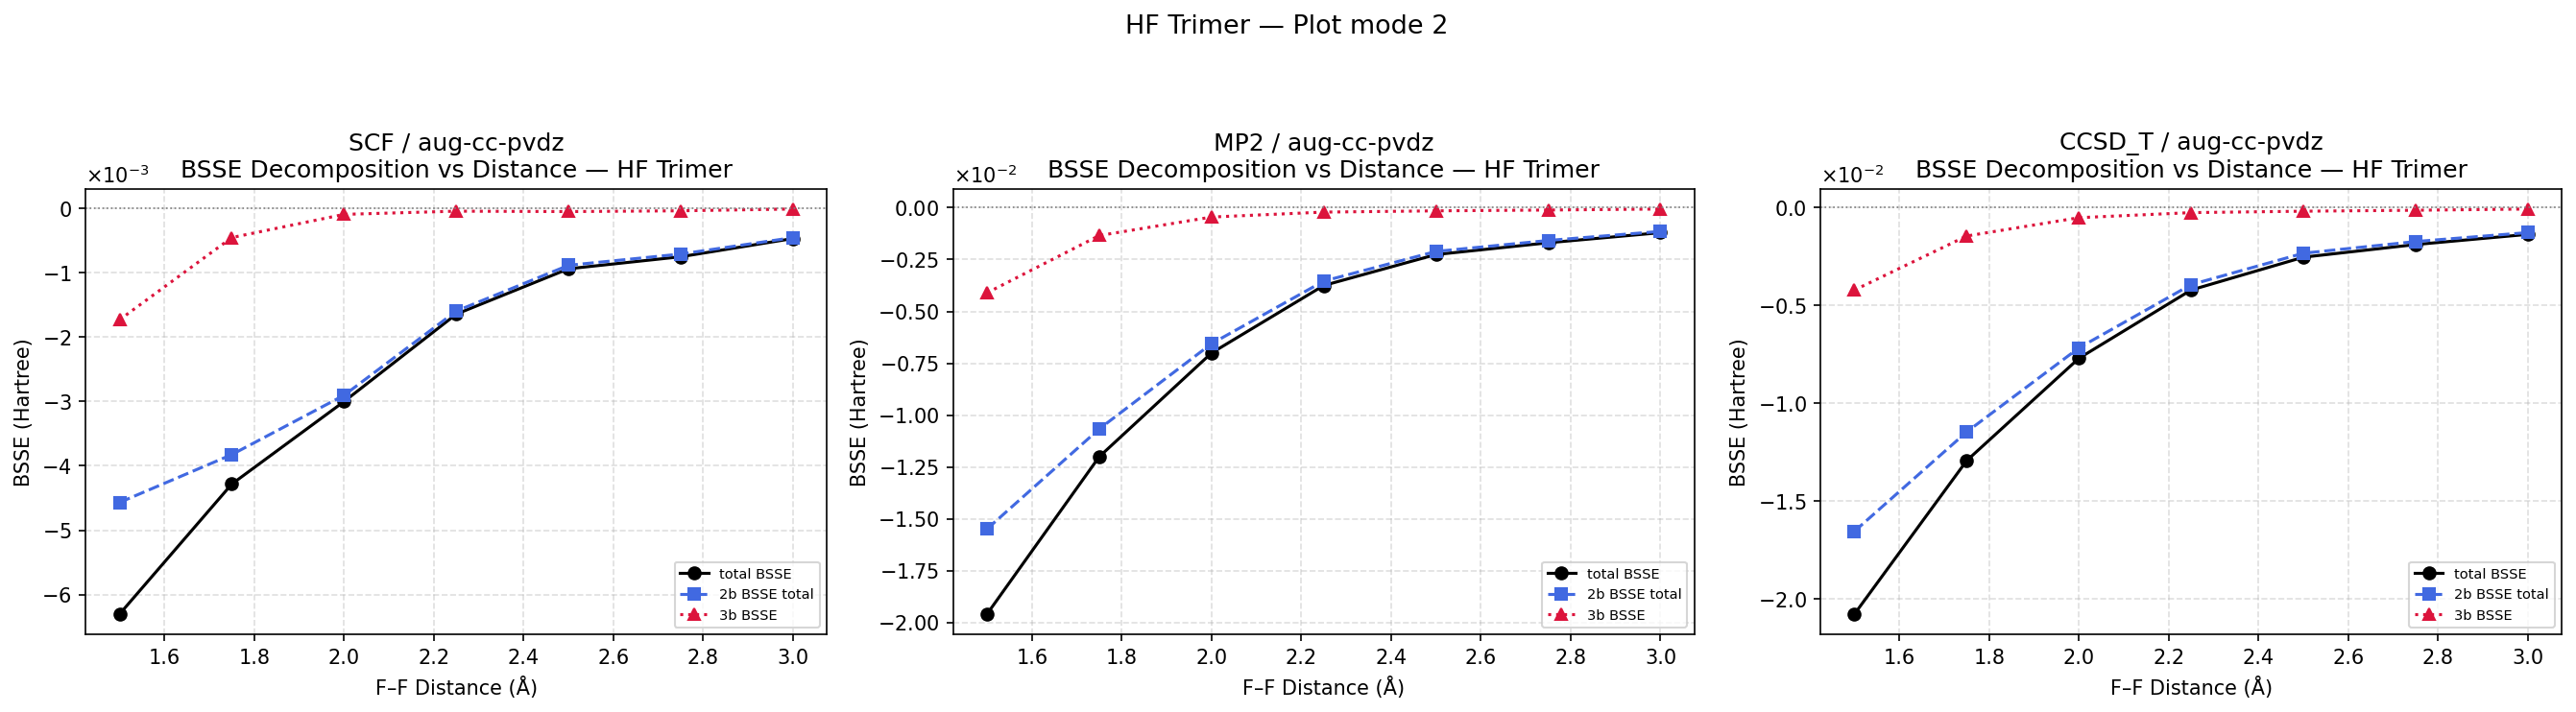
\includegraphics[width=0.7\textwidth]{figures/trimer/HF_trimer/plot2_HF_all_aug-cc-pvdz.png}
    \caption{BSSE body-order decomposition vs F--F distance $R$ for
    the HF trimer at the aug-cc-pVDZ level. Each panel corresponds to
    one level of theory (SCF, MP2, CCSD(T)). Black circles: total
    BSSE; blue dashed squares: 2-body total ($\theta^{(2)}$); red
    dashed triangles: 3-body term ($\theta^{(3)}$). Unlike the Ne and
    \ce{H2O} trimers, a clear gap exists between the total BSSE and
    the 2-body total at all methods and distances, indicating a
    significant 3-body contribution. The 3-body term $\theta^{(3)}$
    is negative at all distances and all levels of theory --- the same
    sign as the 2-body total --- and does not change sign across the
    range of $R$ sampled.}
    \label{fig:hf_trimer_plot2}
\end{figure}

In contrast to the Ne and \ce{H2O} trimers, the total BSSE and the
2-body total are visibly distinct in all three panels. The 3-body
contribution $\theta^{(3)}$ is negative at all distances and all
levels of theory, carrying the same sign as the 2-body total and
adding constructively to it. This behavior --- a large, negative
$\theta^{(3)}$ that never changes sign --- distinguishes the HF
trimer from both Ne (which shows a sign change) and \ce{H2O} (where
$\theta^{(3)}$ is positive and near-negligible).

% TODO: pending PI discussion — physical interpretation of the sign
% and magnitude of theta^(3) in the HF trimer relative to Ne and H2O.

% ----------------------------------------------------------------------
\subsection{Per-Pair Two-Body BSSE}
% ----------------------------------------------------------------------

Figure~\ref{fig:hf_trimer_plot3} resolves the 2-body BSSE into
contributions from each of the three monomer pairs: AB, AC, and BC.

\begin{figure}[!ht]
    \centering
    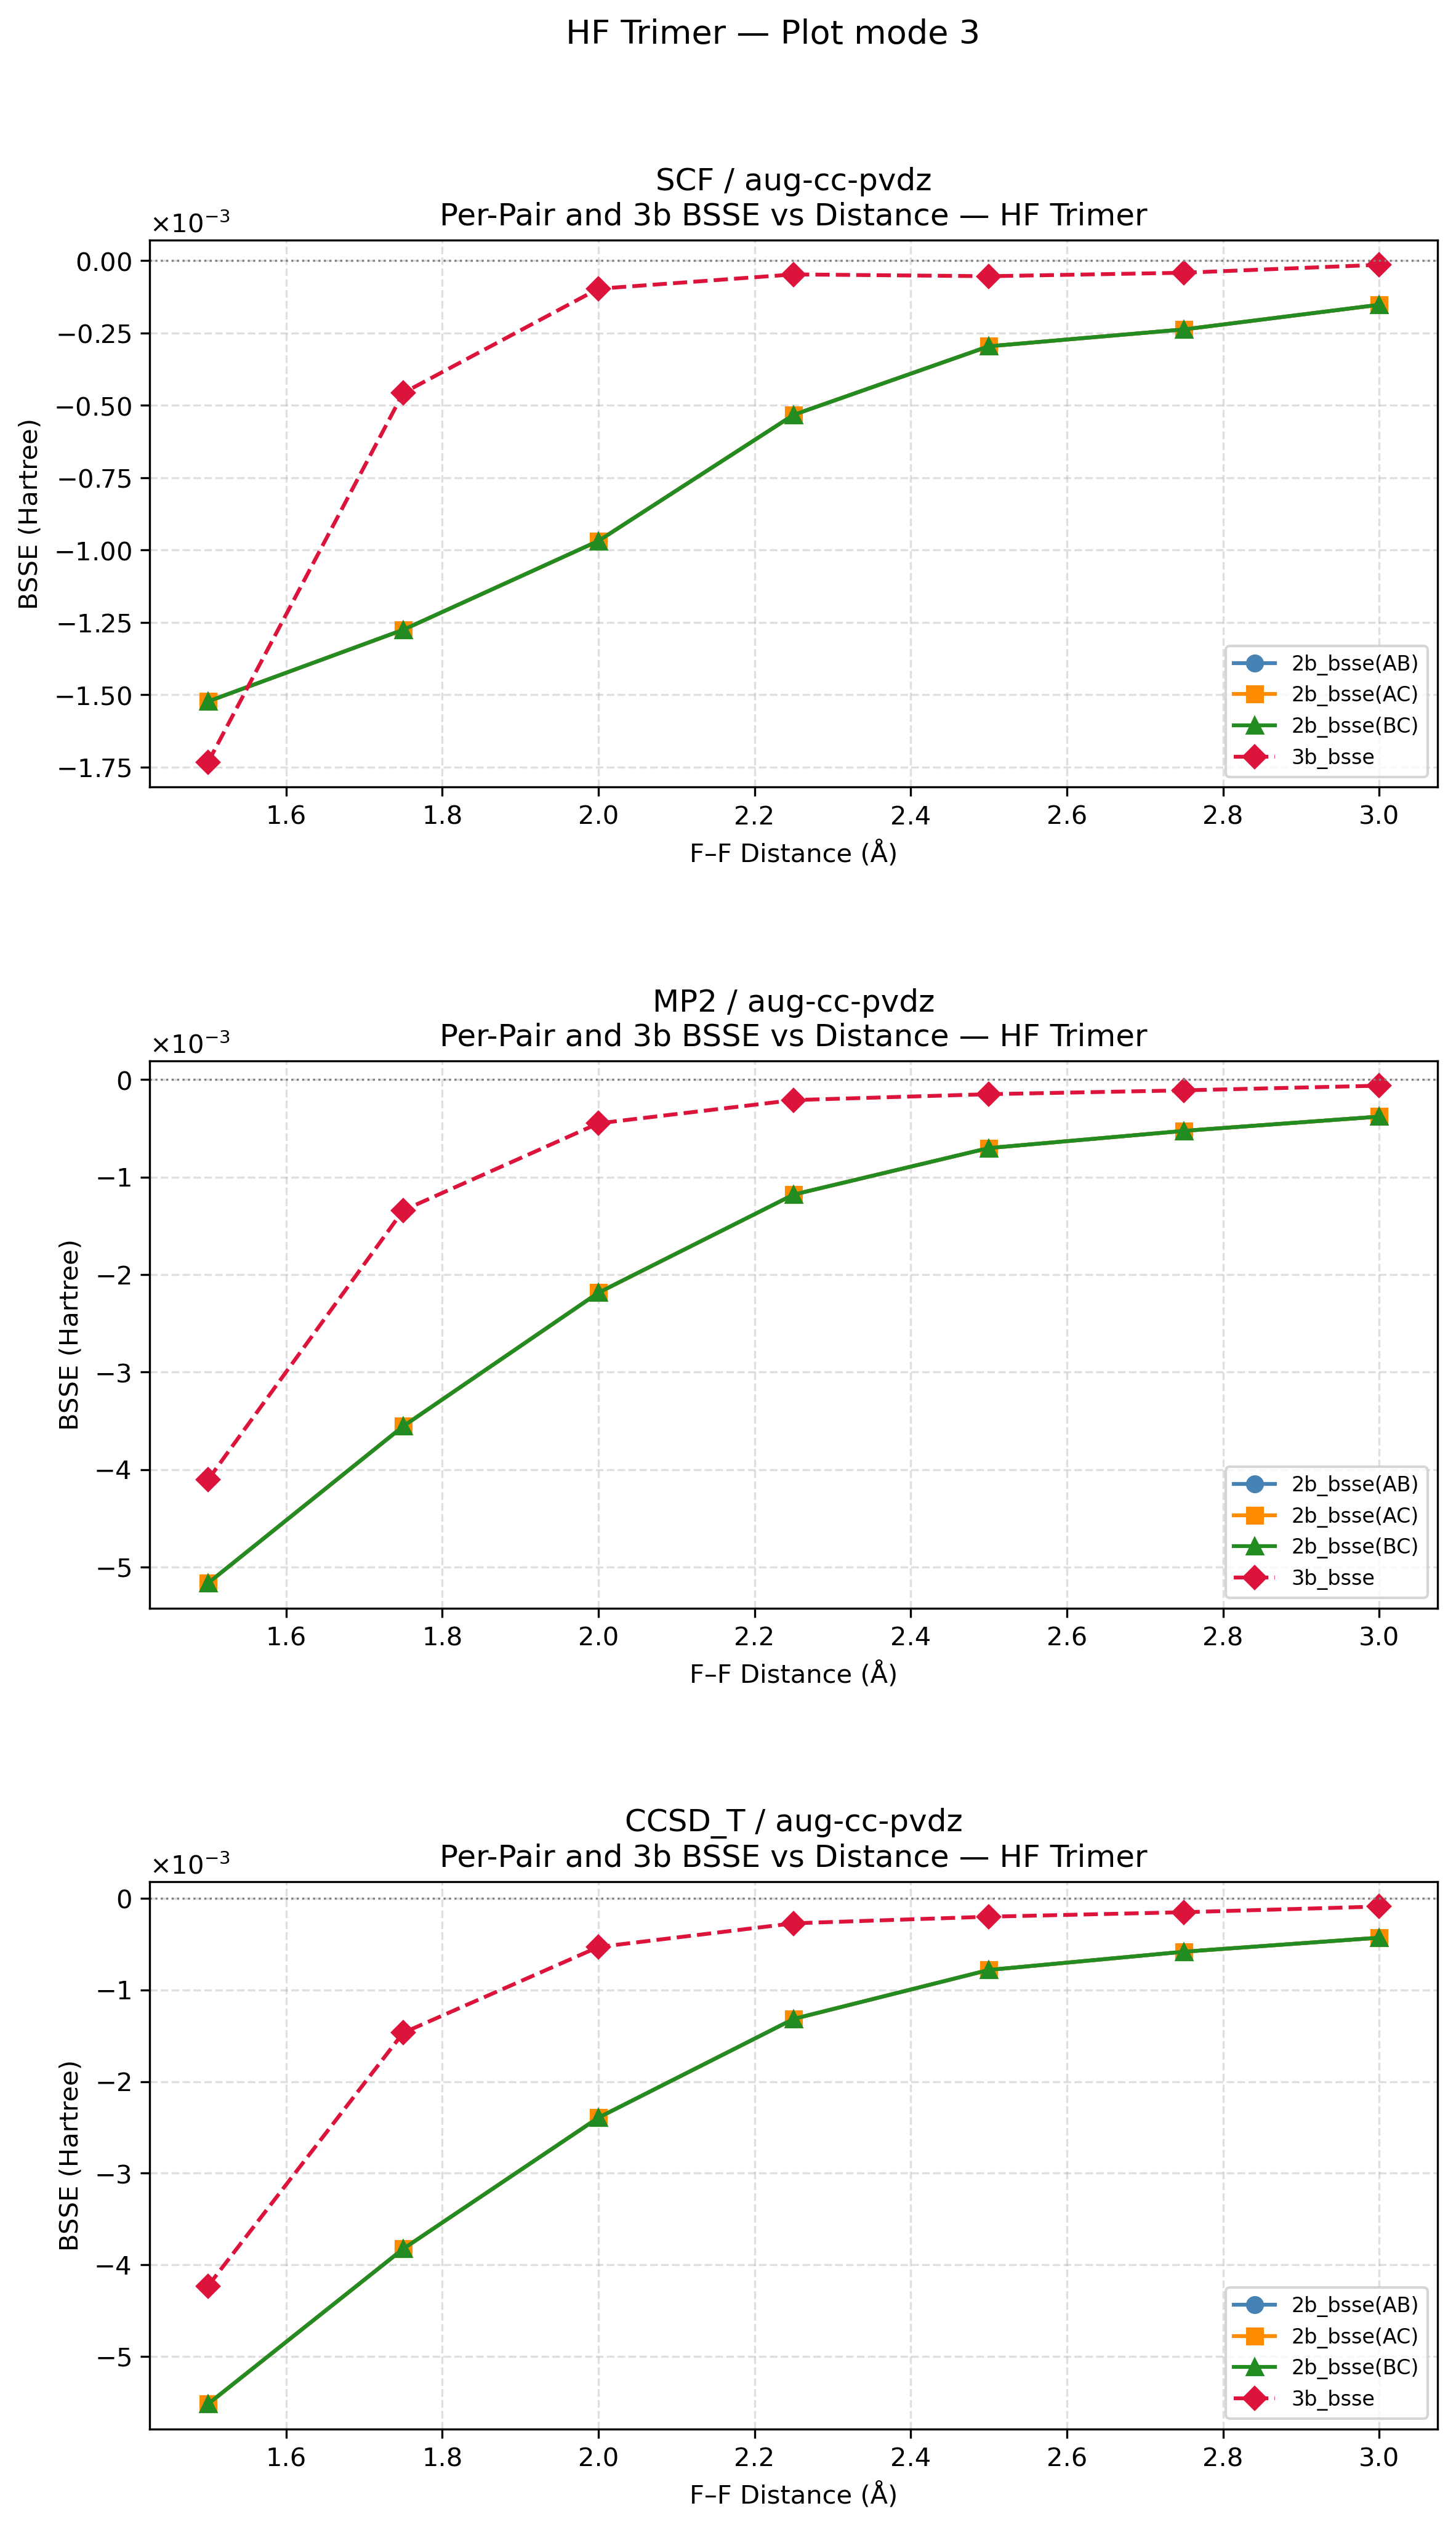
\includegraphics[width=0.7\textwidth]{figures/trimer/HF_trimer/plot3_HF_all_aug-cc-pvdz.png}
    \caption{Per-pair 2-body and 3-body BSSE vs F--F distance $R$
    for the HF trimer at the aug-cc-pVDZ level. Each panel corresponds
    to one level of theory. Blue circles: $\theta^{(2)}$(AB); orange
    squares: $\theta^{(2)}$(AC); green triangles: $\theta^{(2)}$(BC);
    red dashed diamonds: $\theta^{(3)}$. The three pair contributions
    are exactly equal at every distance and every level of theory:
    $\theta^{(2)}(\text{AB}) = \theta^{(2)}(\text{AC}) =
    \theta^{(2)}(\text{BC})$ at all $R$. The 3-body term is negative
    and of comparable magnitude to the individual pair contributions
    at short range.}
    \label{fig:hf_trimer_plot3}
\end{figure}

As with the Ne trimer, the three pair contributions are numerically
identical at every configuration and every level of theory, and the
three symbols lie exactly on top of one another in
Figure~\ref{fig:hf_trimer_plot3}. This reflects the equilateral
arrangement of the fluorine atoms and the equivalence of the three
HF monomers. A notable feature of the HF trimer is the magnitude of
$\theta^{(3)}$ relative to the per-pair contributions: at short range
the 3-body term is comparable in magnitude to a single pair
contribution, a much larger relative 3-body effect than seen in
either Ne or \ce{H2O}.

% TODO: pending PI discussion — physical interpretation of large
% relative 3-body contribution at short range in the HF trimer.

\clearpage

% ----------------------------------------------------------------------
\subsection{Two-Body BSSE Decomposition at $R = \SI{2.25}{\angstrom}$}
% ----------------------------------------------------------------------

Figure~\ref{fig:hf_trimer_plot4} shows the FORM~II decomposition of
the 2-body BSSE at the representative configuration $R =
\SI{2.25}{\angstrom}$ (configuration~3) at the CCSD(T) level.

\begin{figure}[!ht]
    \centering
    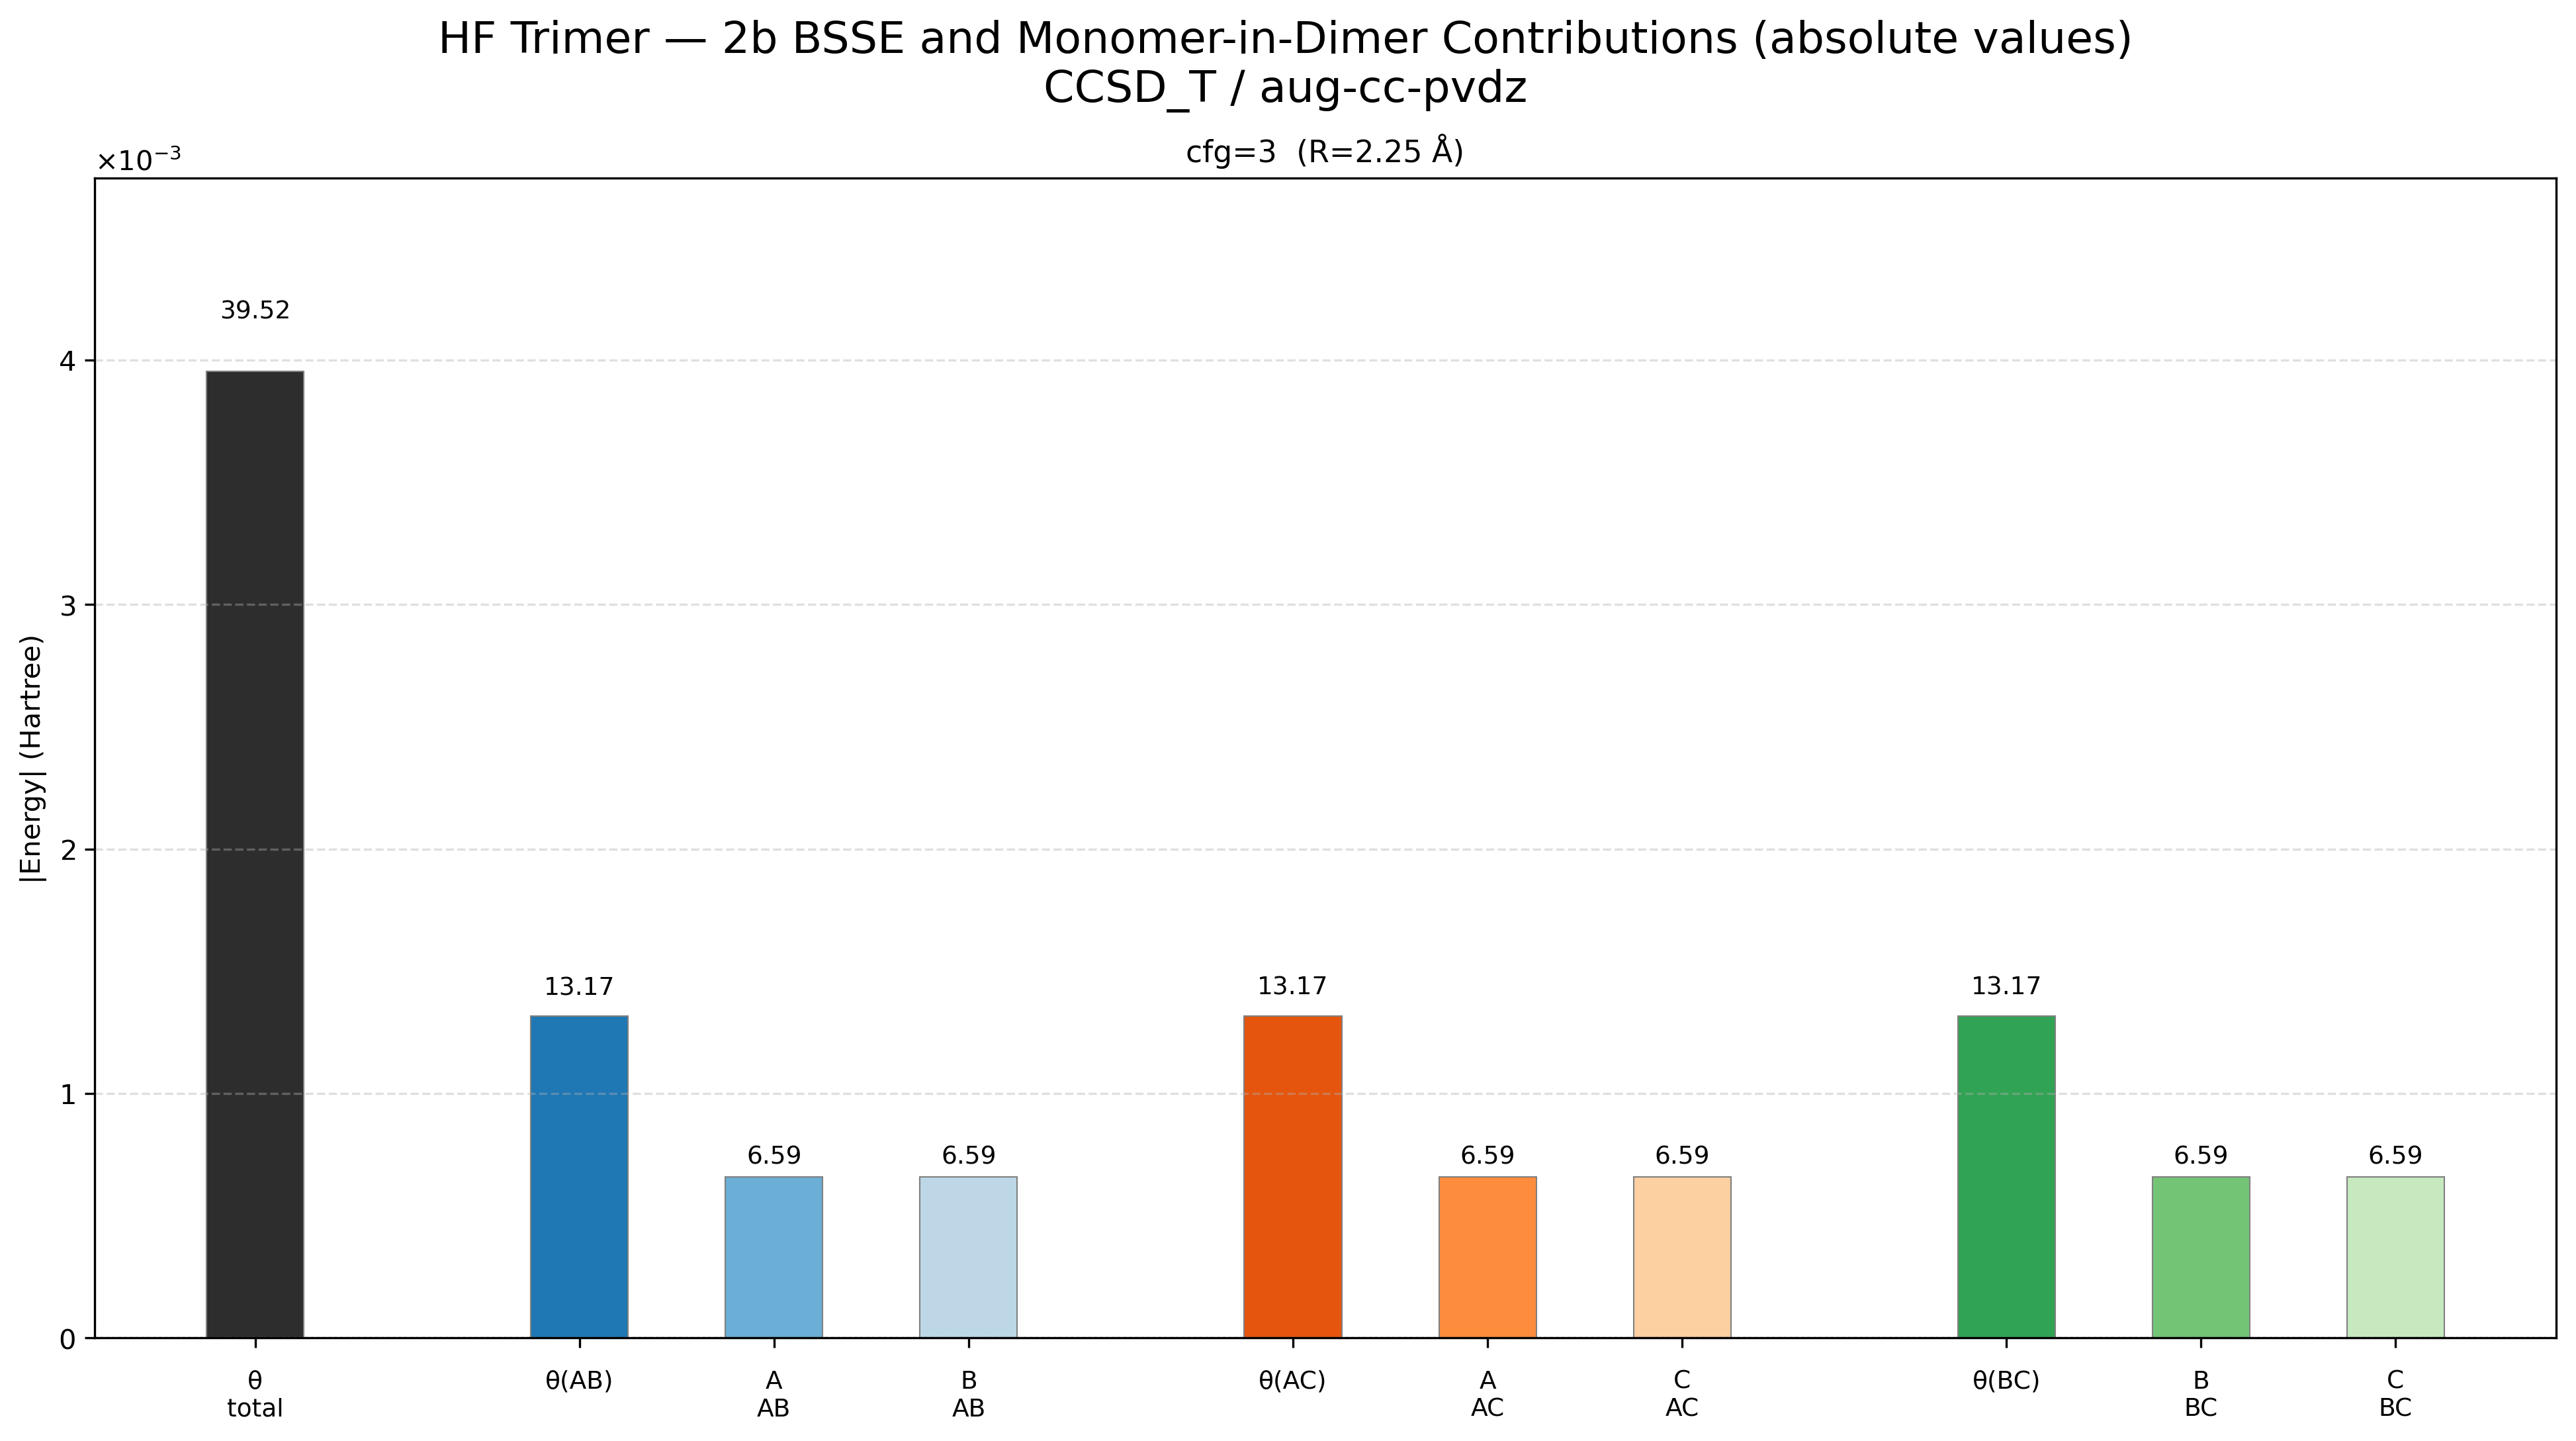
\includegraphics[width=1.0\textwidth]{figures/trimer/HF_trimer/plot4_HF_CCSD_T_aug-cc-pvdz_part4.png}
    \caption{FORM~II decomposition of the 2-body BSSE for the HF
    trimer at $R = \SI{2.25}{\angstrom}$ (configuration~3),
    CCSD(T)/aug-cc-pVDZ. All values are absolute values in units
    of $10^{-3}$~Ha. Black bar: total 2-body BSSE
    $|\theta^{(2)}| = 39.52 \times 10^{-3}$~Ha. For each pair
    (AB, AC, BC) the pair total is $13.17 \times 10^{-3}$~Ha,
    and the two monomer-in-dimer-basis contributions are each
    $6.59 \times 10^{-3}$~Ha. All nine per-pair and per-monomer
    bars are identical, reflecting the equilateral symmetry of
    the HF trimer at this geometry.}
    \label{fig:hf_trimer_plot4}
\end{figure}

At $R = \SI{2.25}{\angstrom}$ all three pair totals are equal:
$|\theta^{(2)}(\text{AB})| = |\theta^{(2)}(\text{AC})| =
|\theta^{(2)}(\text{BC})| = 13.17 \times 10^{-3}$~Ha, and within
each pair the two monomer-in-dimer-basis contributions are also equal
($6.59 \times 10^{-3}$~Ha each). The total 2-body BSSE is three times
the per-pair value: $3 \times 13.17 = 39.52 \times 10^{-3}$~Ha.
Comparing to the Ne trimer at its representative configuration
($10.82 \times 10^{-3}$~Ha), the HF 2-body BSSE is approximately
four times larger at this distance, reflecting the much larger basis
set requirements of the fluorine and hydrogen atoms in a
hydrogen-bonding environment.

% ----------------------------------------------------------------------
\subsection{Three-Body BSSE Decomposition at $R = \SI{2.25}{\angstrom}$}
% ----------------------------------------------------------------------

Figure~\ref{fig:hf_trimer_plot5} shows the FORM~II decomposition of
the 3-body BSSE at the same representative configuration.

\begin{figure}[!ht]
    \centering
    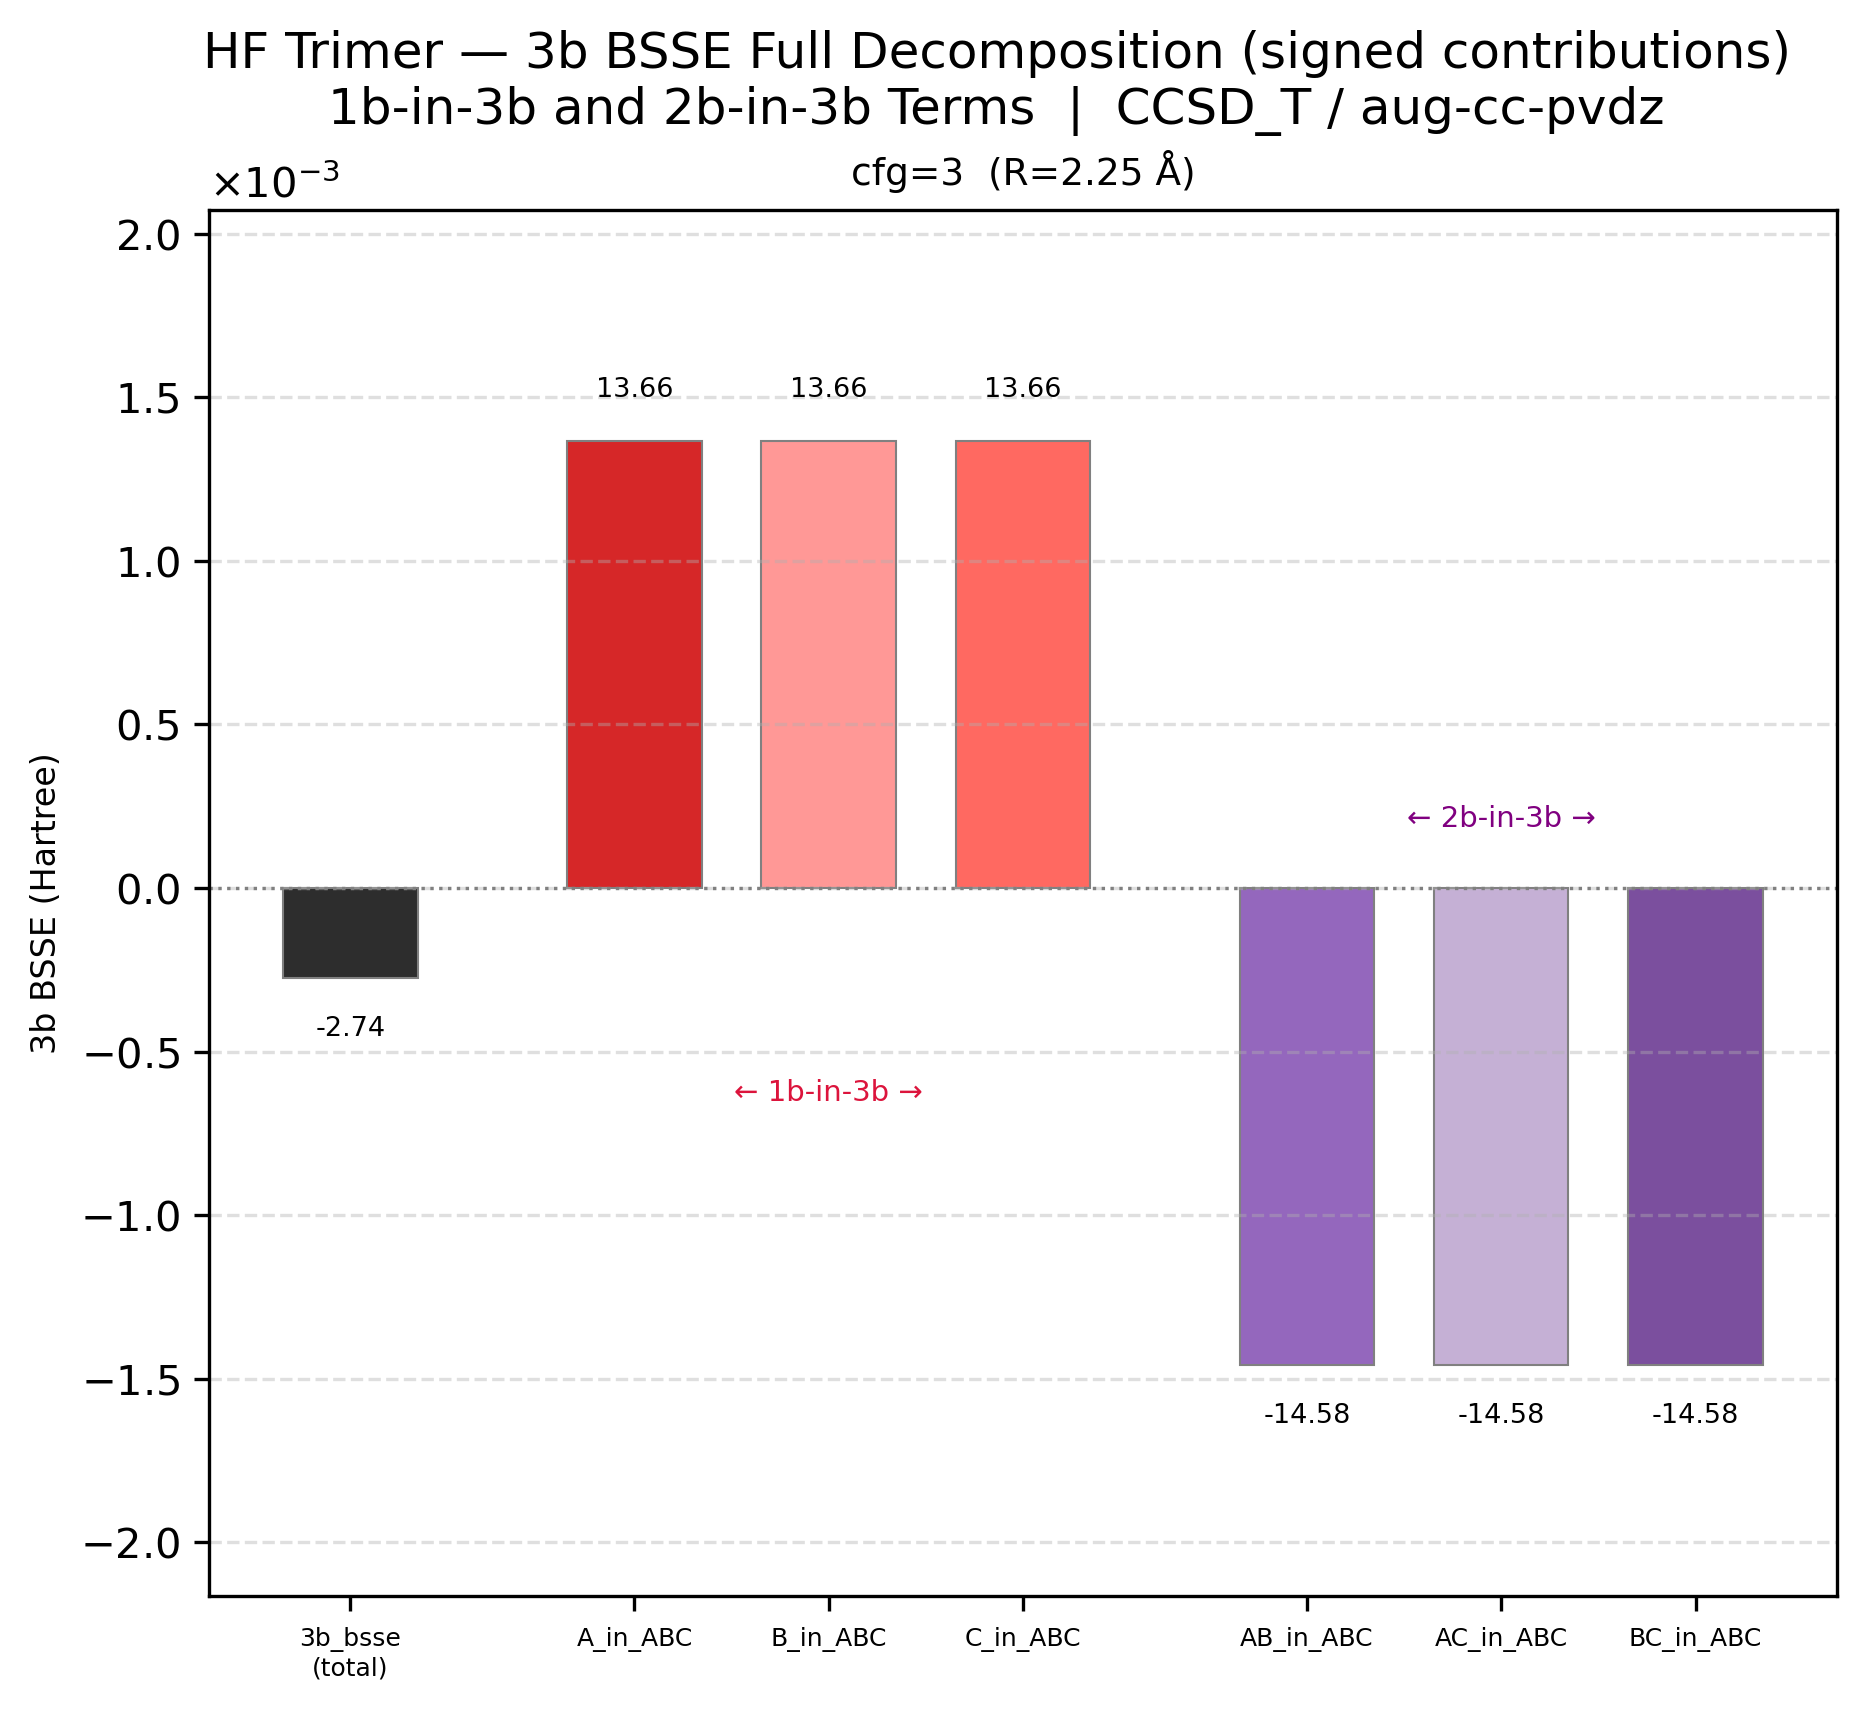
\includegraphics[width=1.0\textwidth]{figures/trimer/HF_trimer/plot5_HF_CCSD_T_aug-cc-pvdz_part4.png}
    \caption{FORM~II decomposition of the 3-body BSSE for the HF
    trimer at $R = \SI{2.25}{\angstrom}$ (configuration~3),
    CCSD(T)/aug-cc-pVDZ. Signed contributions in units of
    $10^{-3}$~Ha. Black bar: total $\theta^{(3)} = -2.74 \times
    10^{-3}$~Ha. Red bars (positive): 1b-in-3b terms
    $\delta(\text{A in ABC}) = \delta(\text{B in ABC}) =
    \delta(\text{C in ABC}) = +13.66 \times 10^{-3}$~Ha.
    Purple bars (negative): 2b-in-3b terms
    $\delta(\text{AB in ABC}) = \delta(\text{AC in ABC}) =
    \delta(\text{BC in ABC}) = -14.58 \times 10^{-3}$~Ha.
    The 2b-in-3b group dominates over the 1b-in-3b group, yielding
    a net negative $\theta^{(3)}$. Note the $\times 10^{-3}$~Ha
    scale --- an order of magnitude larger than the corresponding
    Ne trimer decomposition.}
    \label{fig:hf_trimer_plot5}
\end{figure}

\clearpage

The structure of the 3-body BSSE decomposition for HF mirrors the
pattern seen for Ne and \ce{H2O}: a near-cancellation between the
positive 1b-in-3b terms and the negative 2b-in-3b terms. However,
for HF the 2b-in-3b group dominates more substantially, with each
term ($-14.58 \times 10^{-3}$~Ha) exceeding the corresponding
1b-in-3b term ($+13.66 \times 10^{-3}$~Ha) by approximately 7\%.
This imbalance yields a net $\theta^{(3)} = -2.74 \times 10^{-3}$~Ha,
which is negative at this configuration and at all configurations
sampled (Figure~\ref{fig:hf_trimer_plot2}). All bars within each
group are exactly equal, confirming the equilateral symmetry of the
cluster. The overall scale --- $10^{-3}$~Ha versus $10^{-4}$~Ha for
Ne --- underscores the much larger 3-body BSSE in the HF trimer.

% ----------------------------------------------------------------------
\subsection{Key Findings}
% ----------------------------------------------------------------------

\begin{finding_box}
\textbf{The 3-body BSSE is large and negative at all HF trimer
configurations.}
Unlike the Ne trimer (where $\theta^{(3)}$ changes sign with $R$) and
the \ce{H2O} trimer (where $\theta^{(3)}$ is positive and
near-negligible), the HF trimer shows a large negative $\theta^{(3)}$
at every F--F distance and every level of theory sampled. The 3-body
contribution adds constructively to the 2-body total, making the total
BSSE significantly larger than the 2-body term alone. At the shortest
distance ($R = \SI{1.5}{\angstrom}$) the $|\theta^{(3)}/\theta^{(2)}|$
ratio reaches approximately 25\% at the CCSD(T) level.
\end{finding_box}

\begin{finding_box}
\textbf{The FORM~II decomposition shows a persistent 2b-in-3b
dominance.}
At all configurations the 3-body BSSE arises from a near-cancellation
between the positive 1b-in-3b and negative 2b-in-3b FORM~II delta
terms, with the 2b-in-3b group always larger in magnitude. At the
representative configuration ($R = \SI{2.25}{\angstrom}$, CCSD(T))
each 2b-in-3b term is $-14.58 \times 10^{-3}$~Ha and each 1b-in-3b
term is $+13.66 \times 10^{-3}$~Ha, yielding a net
$\theta^{(3)} = -2.74 \times 10^{-3}$~Ha. This contrasts with the
Ne trimer at longer range, where the 1b-in-3b group comes to dominate
and $\theta^{(3)}$ turns positive.
% TODO: pending PI discussion — physical interpretation of persistent
% 2b-in-3b dominance and sign difference relative to Ne trimer.
\end{finding_box}

\clearpage

%-----------------------------------------------------------------------
% Chapter 6 — Trimer: BSSE vs Interaction Energy
%-----------------------------------------------------------------------
% \chapter{\ce{H2O} Trimer: BSSE and Interaction Energy}
% \input{sections/trimer_interaction}

%-----------------------------------------------------------------------
% Chapter 7 — Next Steps
%-----------------------------------------------------------------------
% \chapter{Next Steps and Outlook}
% \input{sections/next_steps}

%-----------------------------------------------------------------------
% References
%-----------------------------------------------------------------------
\printbibliography[heading=bibintoc, title={References}]

\end{document}
